\documentclass[a4paper, 11 pt]{report}

\usepackage{makeidx}
\usepackage[latin1]{inputenc}
\usepackage[english]{babel}
\usepackage{indentfirst}
\usepackage{graphicx}
\usepackage{subfigure}
\usepackage{mathtools}
\usepackage[retainorgcmds]{IEEEtrantools}
\usepackage{multirow}
\usepackage{array}
%\usepackage{mhchem}
\usepackage{booktabs}
%\usepackage{psfrag}
\usepackage[hypcap=true]{caption}
\usepackage[bookmarks=true,hyperfootnotes=false]{hyperref}
\hypersetup{
	colorlinks=true,
	linkcolor=red,
	anchorcolor=red,
	citecolor=red,
	urlcolor=red,
	%linktocpage=true
	pdftitle={THGEM characterization},
	pdfauthor={I. Ciraldo, G.A. Brischetto}
}

\newcommand{\Vind}{$\Delta V_{ind}$}
\newcommand{\Vthgem}{$\Delta V_{TH}$}
\newcommand{\Vdrift}{$ \Delta V_{drift}$}
\newcommand{\Eind}{E/p_${ind}$}
\newcommand{\Ethgem}{E/p$_{TH}$}
\newcommand{\Edrift}{E/p$_{drift}$}

\newcommand{\ibf}{$I_{bf}$}
\newcommand{\ibeam}{$I_{beam}$}

\title{\bf {\huge FULL and ROW THGEM characterization} }
\author{G.A. Brischetto, I. Ciraldo, D. Torresi}
\date{26 March 2020}



\begin{document}

\maketitle

\section*{Abstract}
In the present report the characterization of the tracker prototype using different kind of THGEM is 
described. The main parameters that have been explored are: the THGEM voltage, the drift voltage,
the induction voltage, the gas pressure and the rate of the incident particles.
\tableofcontents

\chapter{Experimental setup}

The gas tracker have been tested in a gas chamber located along the TeBe beam line that is shown in Fig. 
\ref{fig:TeBeline}.
\begin{figure}
	\centering
	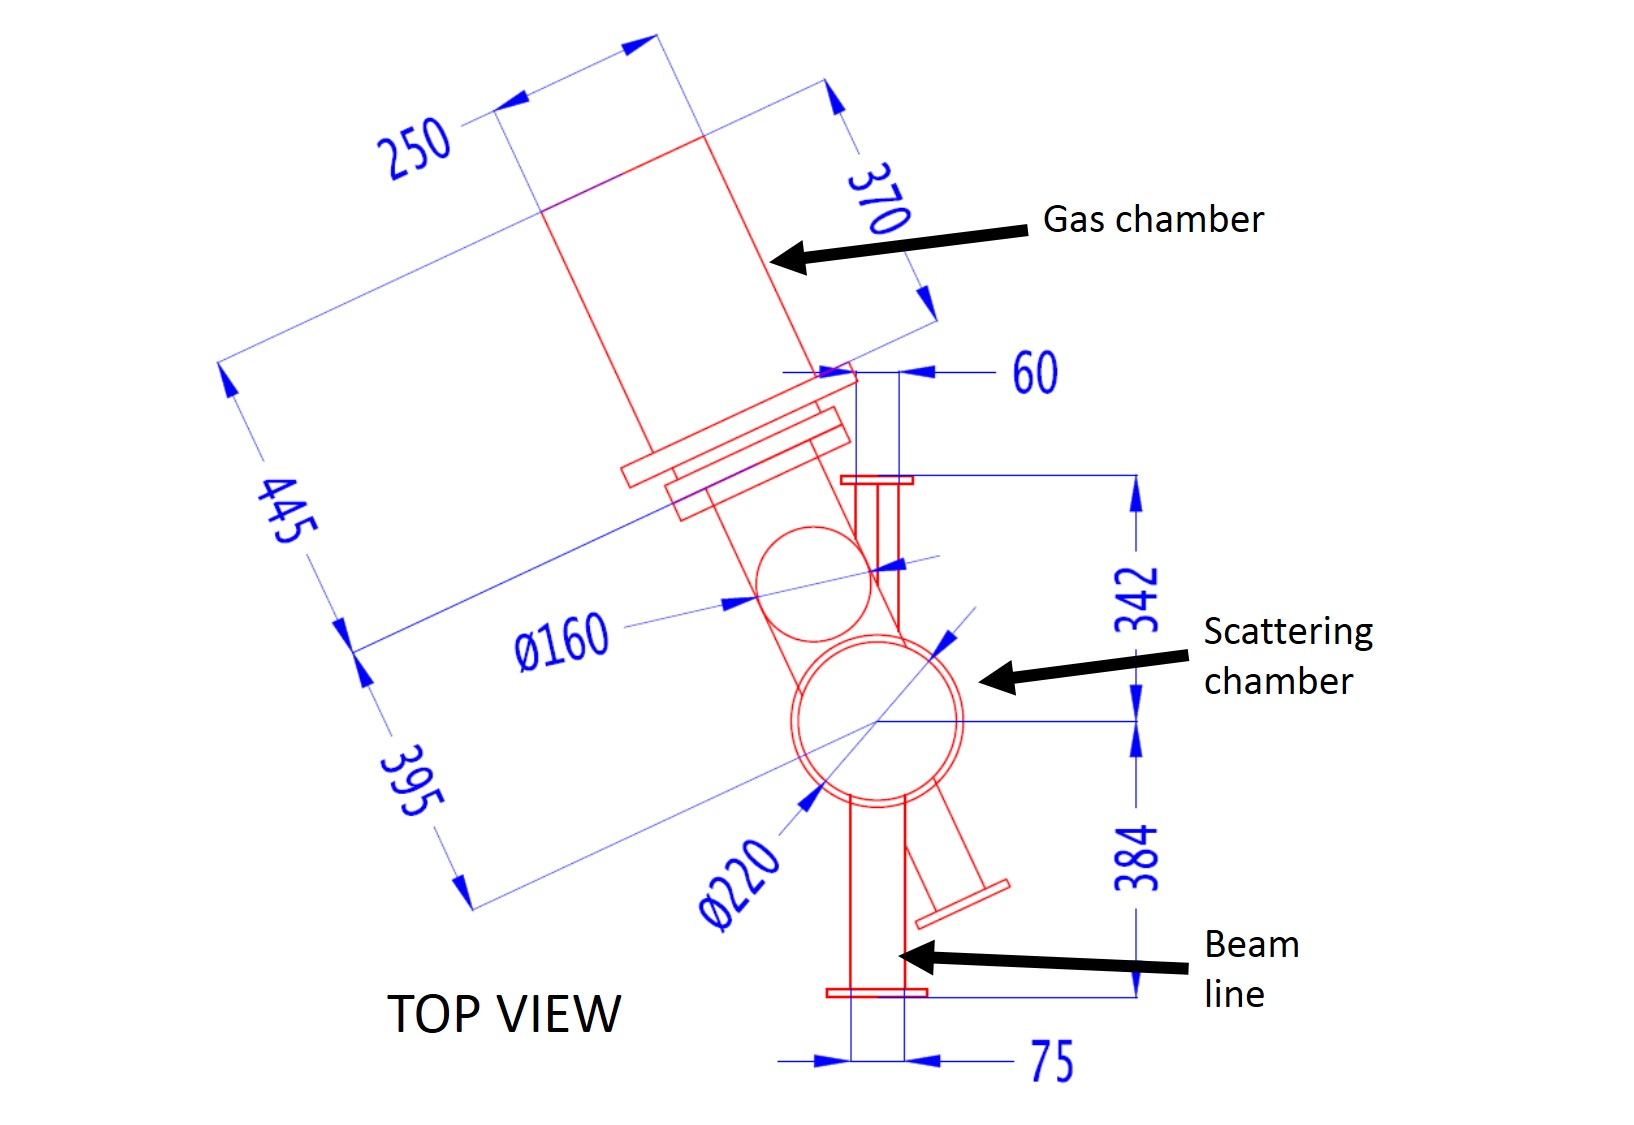
\includegraphics[width=0.9\textwidth]{Immagini/TeBe_scheme.jpg}
	\caption{Sketch of the TeBe beam line.}
	\label{fig:TeBeline}
\end{figure}
The gas chamber is isolated from the high vacuum beam line by mean of a thin Mylar window (2.5 or 6 
$\mu m$ thick) or by a few mm thick aluminum plate. This last is used just during the test with 
$\alpha$-source that is located inside the gas chamber itself. The gas chamber is located at an 
angle of 30$^{\circ}$ respect to the beam direction. The window is located at about 47 cm from the 
target position. The window is \textcolor{red}{ 120 mm large and 100 mm high}.\\

%aggiungere sezione sul sistema da vuoto
 
A slow control system allow to fill the gas chamber with at a given pressure with a constant
flux of gas up to 145 sccm\footnote{Standard Cubic Centimeter per Minute.}.  
Up to now all the test have been performed using isobutane ($\mbox{C}_4\mbox{H}_{10}$) with a 
purity of 99.95\% at four different pressure: 10, 20, 30 and 40~mbar and with the maximum 
available flux, i.e. 145~sccm.\\

The alpha source used during the test is the is a 55 kBq $^{241}Am$ source. A shutter remotely 
controlled is used to allow (open) or prevent (close) $\alpha$-particles from enter the tracker.\\
The rate of $\alpha$-particles entering the tracker after the shutter is 140 pps (particles per 
second), the shutter cut a solid angle of $3.2\cdot10^{-2}$ sr corresponding to a cone with
an opening angle\footnote{It is the angle betweenthe axis and the boreder.} of $\theta/2=7.26^{\circ}$.\\
% http://goldbook.iupac.org/terms/view/S05971         sradiante ->sr

To supply the required voltages a CAEN system on a CAEN SY5527 mainframe with an A1515 board 
is used (see Sec. \ref{sec:bias}). This system allows also the measurements of the currents flowing in each the power unit.\\

Due to the low sensitivity of the ammeter integrated in the CAEN power supply a more sensitive 
picoammeter have been used, it is called PICO and it was designed and built at INFN-NA.
It is capable to measure the currents with an accuracy of the order of tenth of pA
while the integrated CAEN ammeter has an accuracy of about 2 nA.


\section{Tracker prototype}
\label{sec:prototype}
The tracker prototype consists in one module (one of the 8 final modules) that has the same 
structure as the final FPD but is smaller in the dispersive direction.\\
The active volume of the detector is 107$\times$107$\times$185 mm$^{3}$. While the full size 
nothing excluded is of about 180$\times$200$\times$215 mm$^{3}$. 

An electric scheme of the prototype is shown in Figure~\ref{fig:schema_apparato_2}.\\ 
The {\bf drift region}, delimited by the cathode and the multiplication stage, is 185 mm deep, it is
designed to set a uniform electric field. A partition made of 35 double rings of wires connect 
the edge of the cathode with the edge of the multiplication region. The rings are 5 mm distant and 
in between there are four 10 M$\Omega$ resistors connected in parallel so the resistance is 
2.5~M$\Omega$. The total resistance of the partition is 87.5 M$\Omega$. The presence of this 
partition generate a current of several $\mu$A in the chatode and in the bottom of the THGEM also 
in steady condition (i.e. no particles crossing the drift region). The drift region is filled with 
gas at low pressure (10-100 mbar). The gas filling the drift region should have a high drift 
velocity in order to guarantee a fast collection of the charge and should manifest a saturation of 
the drift velocity with the electrical field applied.\\
The {\bf multiplication stage} is based on multiple THGEM, described in the next subsection.\\
The {\bf induction region} is delimited by the top of the THGEM and the anode and is 1 mm deep. 
The electrons emerging from the multiplication region are directed towards a segmented anode made 
of 144 strips 750 $\mu$m large\footnote{The capacitance of a single strip is roughly 22 pF.}. 
Anyway during the test with ammeter the segmented anode was replaced by an not-segmented anode, 
that is a whole metallized layer with the same mechanical size of the segmented anode.
\begin{figure}
	\centering
	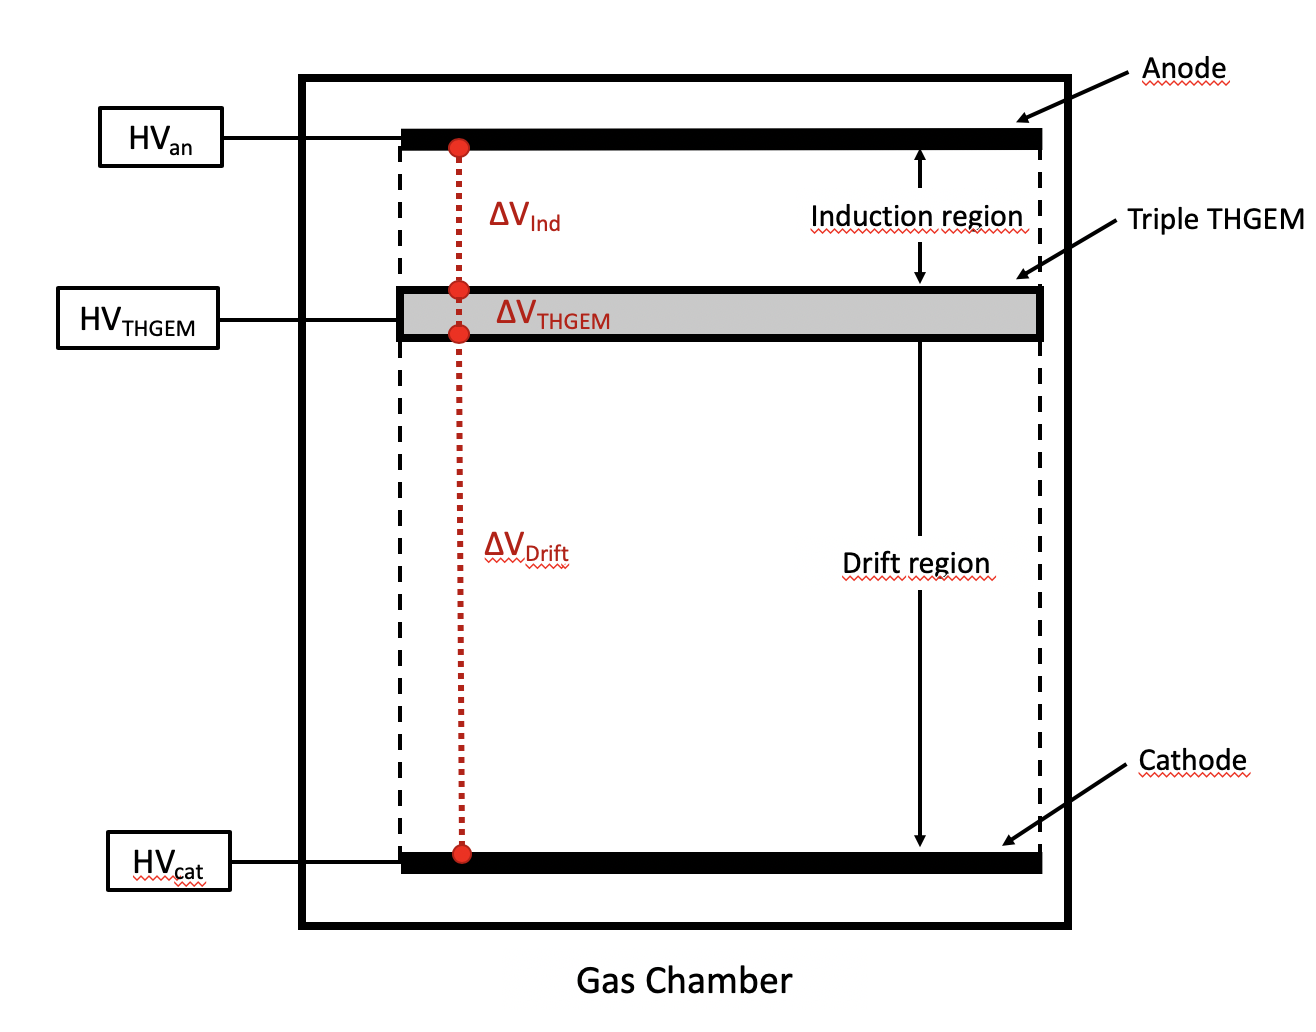
\includegraphics[width=0.9\textwidth]{Immagini/schema_apparato_2.png}
	\caption{Sketch of the Prototype.}
	\label{fig:schema_apparato_2}
\end{figure}
\begin{figure}[htbp]
	\centering
	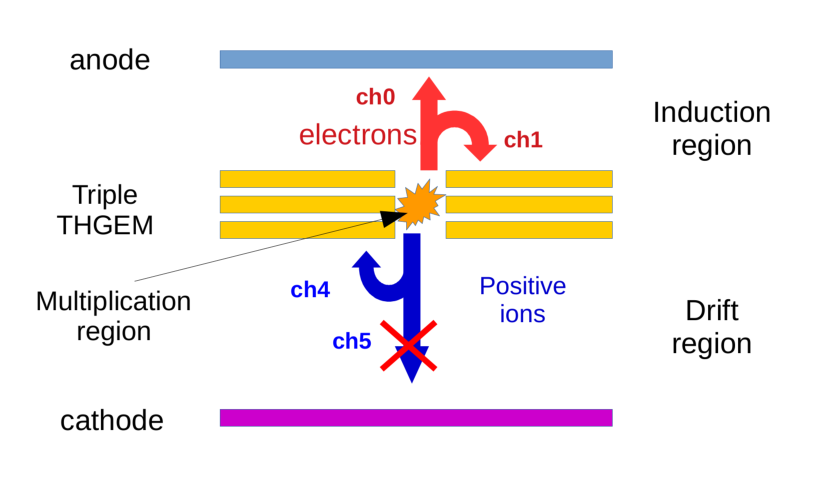
\includegraphics[width=0.7\textwidth]{Immagini/THGEMScheme.pdf}
	\caption{Cartoon of the flows of positive ions and electrons in the tracker prototype.}
	\label{fig:THGEMscheme}
\end{figure}

\section{THGEM}
Two multiple THGEM have been used in the test. Both of them are made of three layers, but they show 
different hole pattern and also different executive details since have been produced by two 
different manufacturers.\\
In the first one, referred to as FULL THGEM \textbf{F10} (Figure~\ref{fig:full_thgem}), the holes 
are uniformly distributed over the active surface; in the second one, called ROW THGEM \textbf{R1} 
(Figure~\ref{fig:row_thgem}), the holes are arranged in five rows.\\
The main characteristics of the two prototypes are shown in Table~\ref{tab:thgem}.\\
The main difference are: the hole pattern, the thickness of the board, the size of the 
rim and the diameter of the hole.
\begin{table} [h!]
   \begin{center}
   \renewcommand{\arraystretch}{1.2}
      \begin{tabular}{|c|c|c|}
        \hline 
		& \textbf{F10} 	& \textbf{R1} \\ 
        \hline 
        Substrate material*			 & Ceramic SD103K 	& PCB  \\ 
        \hline 
        Finish board thickness* [mm] & 1.4 $\pm$ 0.1 	& 1.28 \\ 
        \hline 
        Dimension [$\mbox{mm}^2$] 	 & 107$\times$107 	& 107$\times$107 \\ 
        \hline 
        Rim size* [mm] 				 & 0.1 				& 0.2  \\ 
        \hline  
        Rows 						 & 143$\times$143 	& 5 \\ 
        \hline 
        Holes 						 & 20449 			& 143 \\ 
        \hline 
        Hole diameter* [mm] 		 & 0.30 $\pm$ 0.05 	& 0.280 \\ 
        \hline
        Hole spacing 				 & 0.75 			& 0.75 \\ 
        \hline
      \end{tabular} 
   \end{center}
   \caption{The main characteristics of the two type of THGEM tested. The star highlights
   the characteristics that are different between the two THGEM.} \label{tab:thgem}
\end{table}

\begin{figure}
	\centering
		\subfigure[]{
		 \label{fig:full_thgem}
		 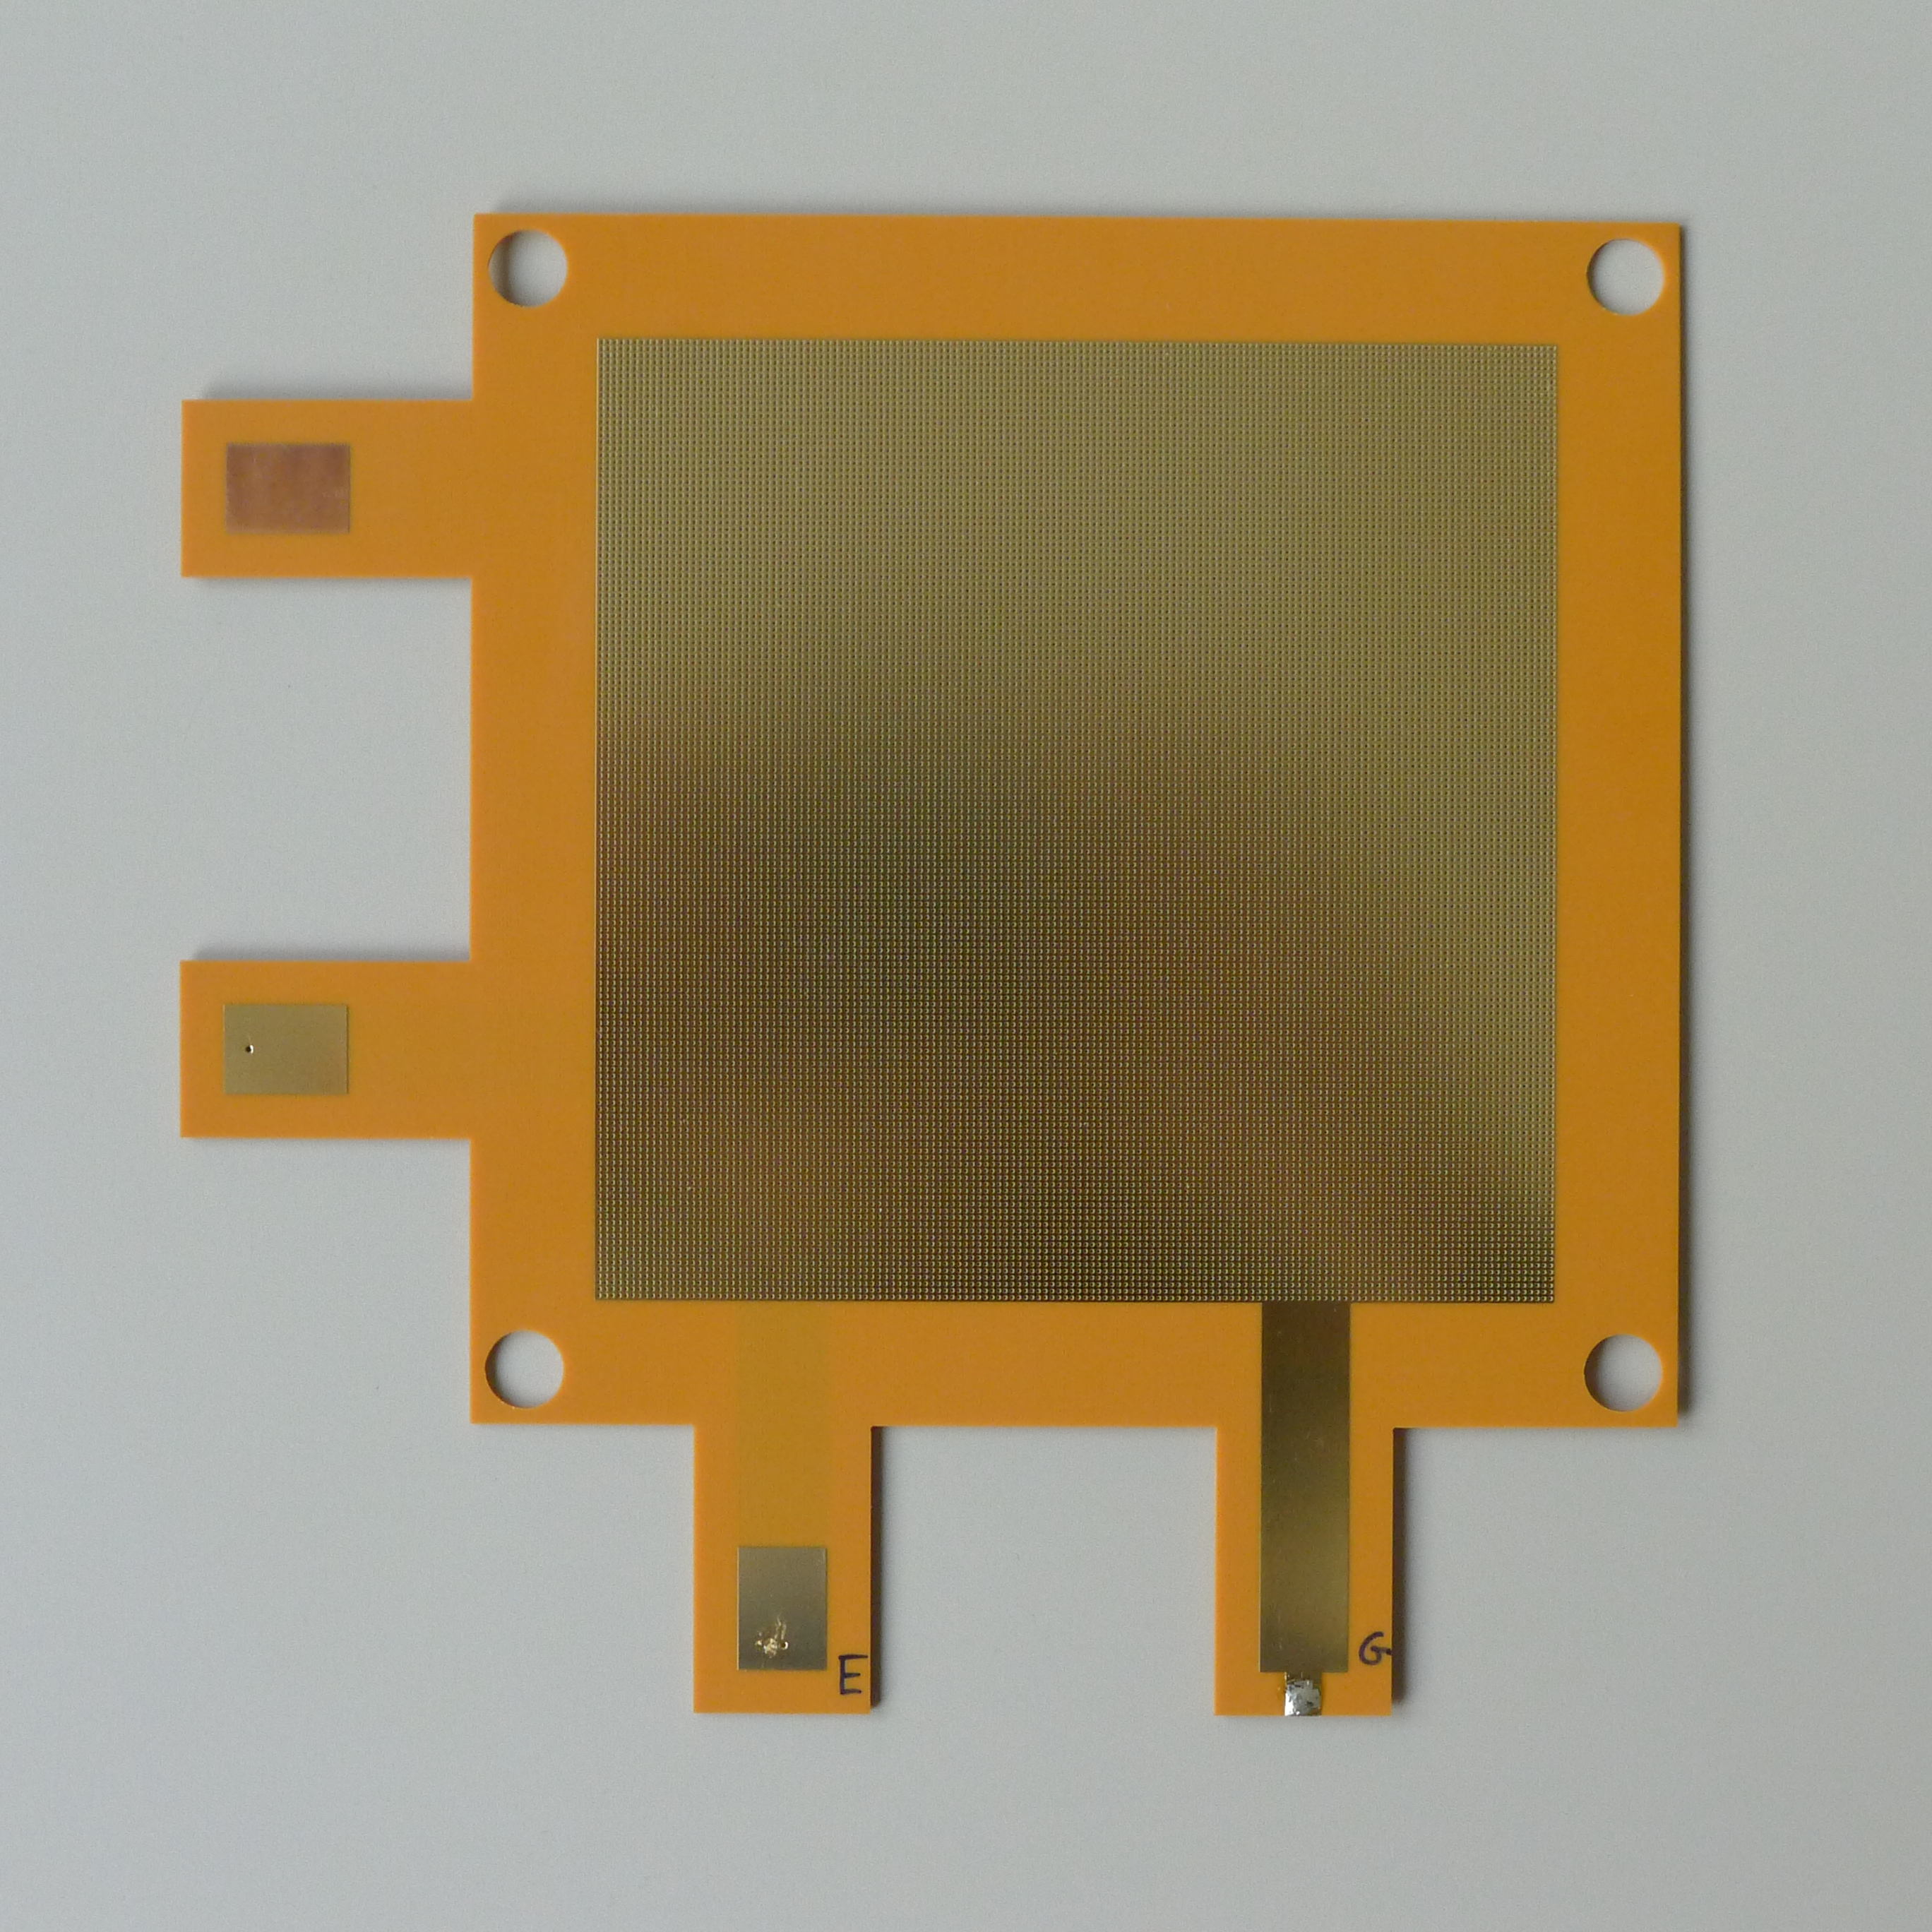
\includegraphics[width=0.45\textwidth]{Immagini/full_thgem.JPG}}
		\hspace{5pt}
		\subfigure[]{
		 \label{fig:full_thgem_holes}
		 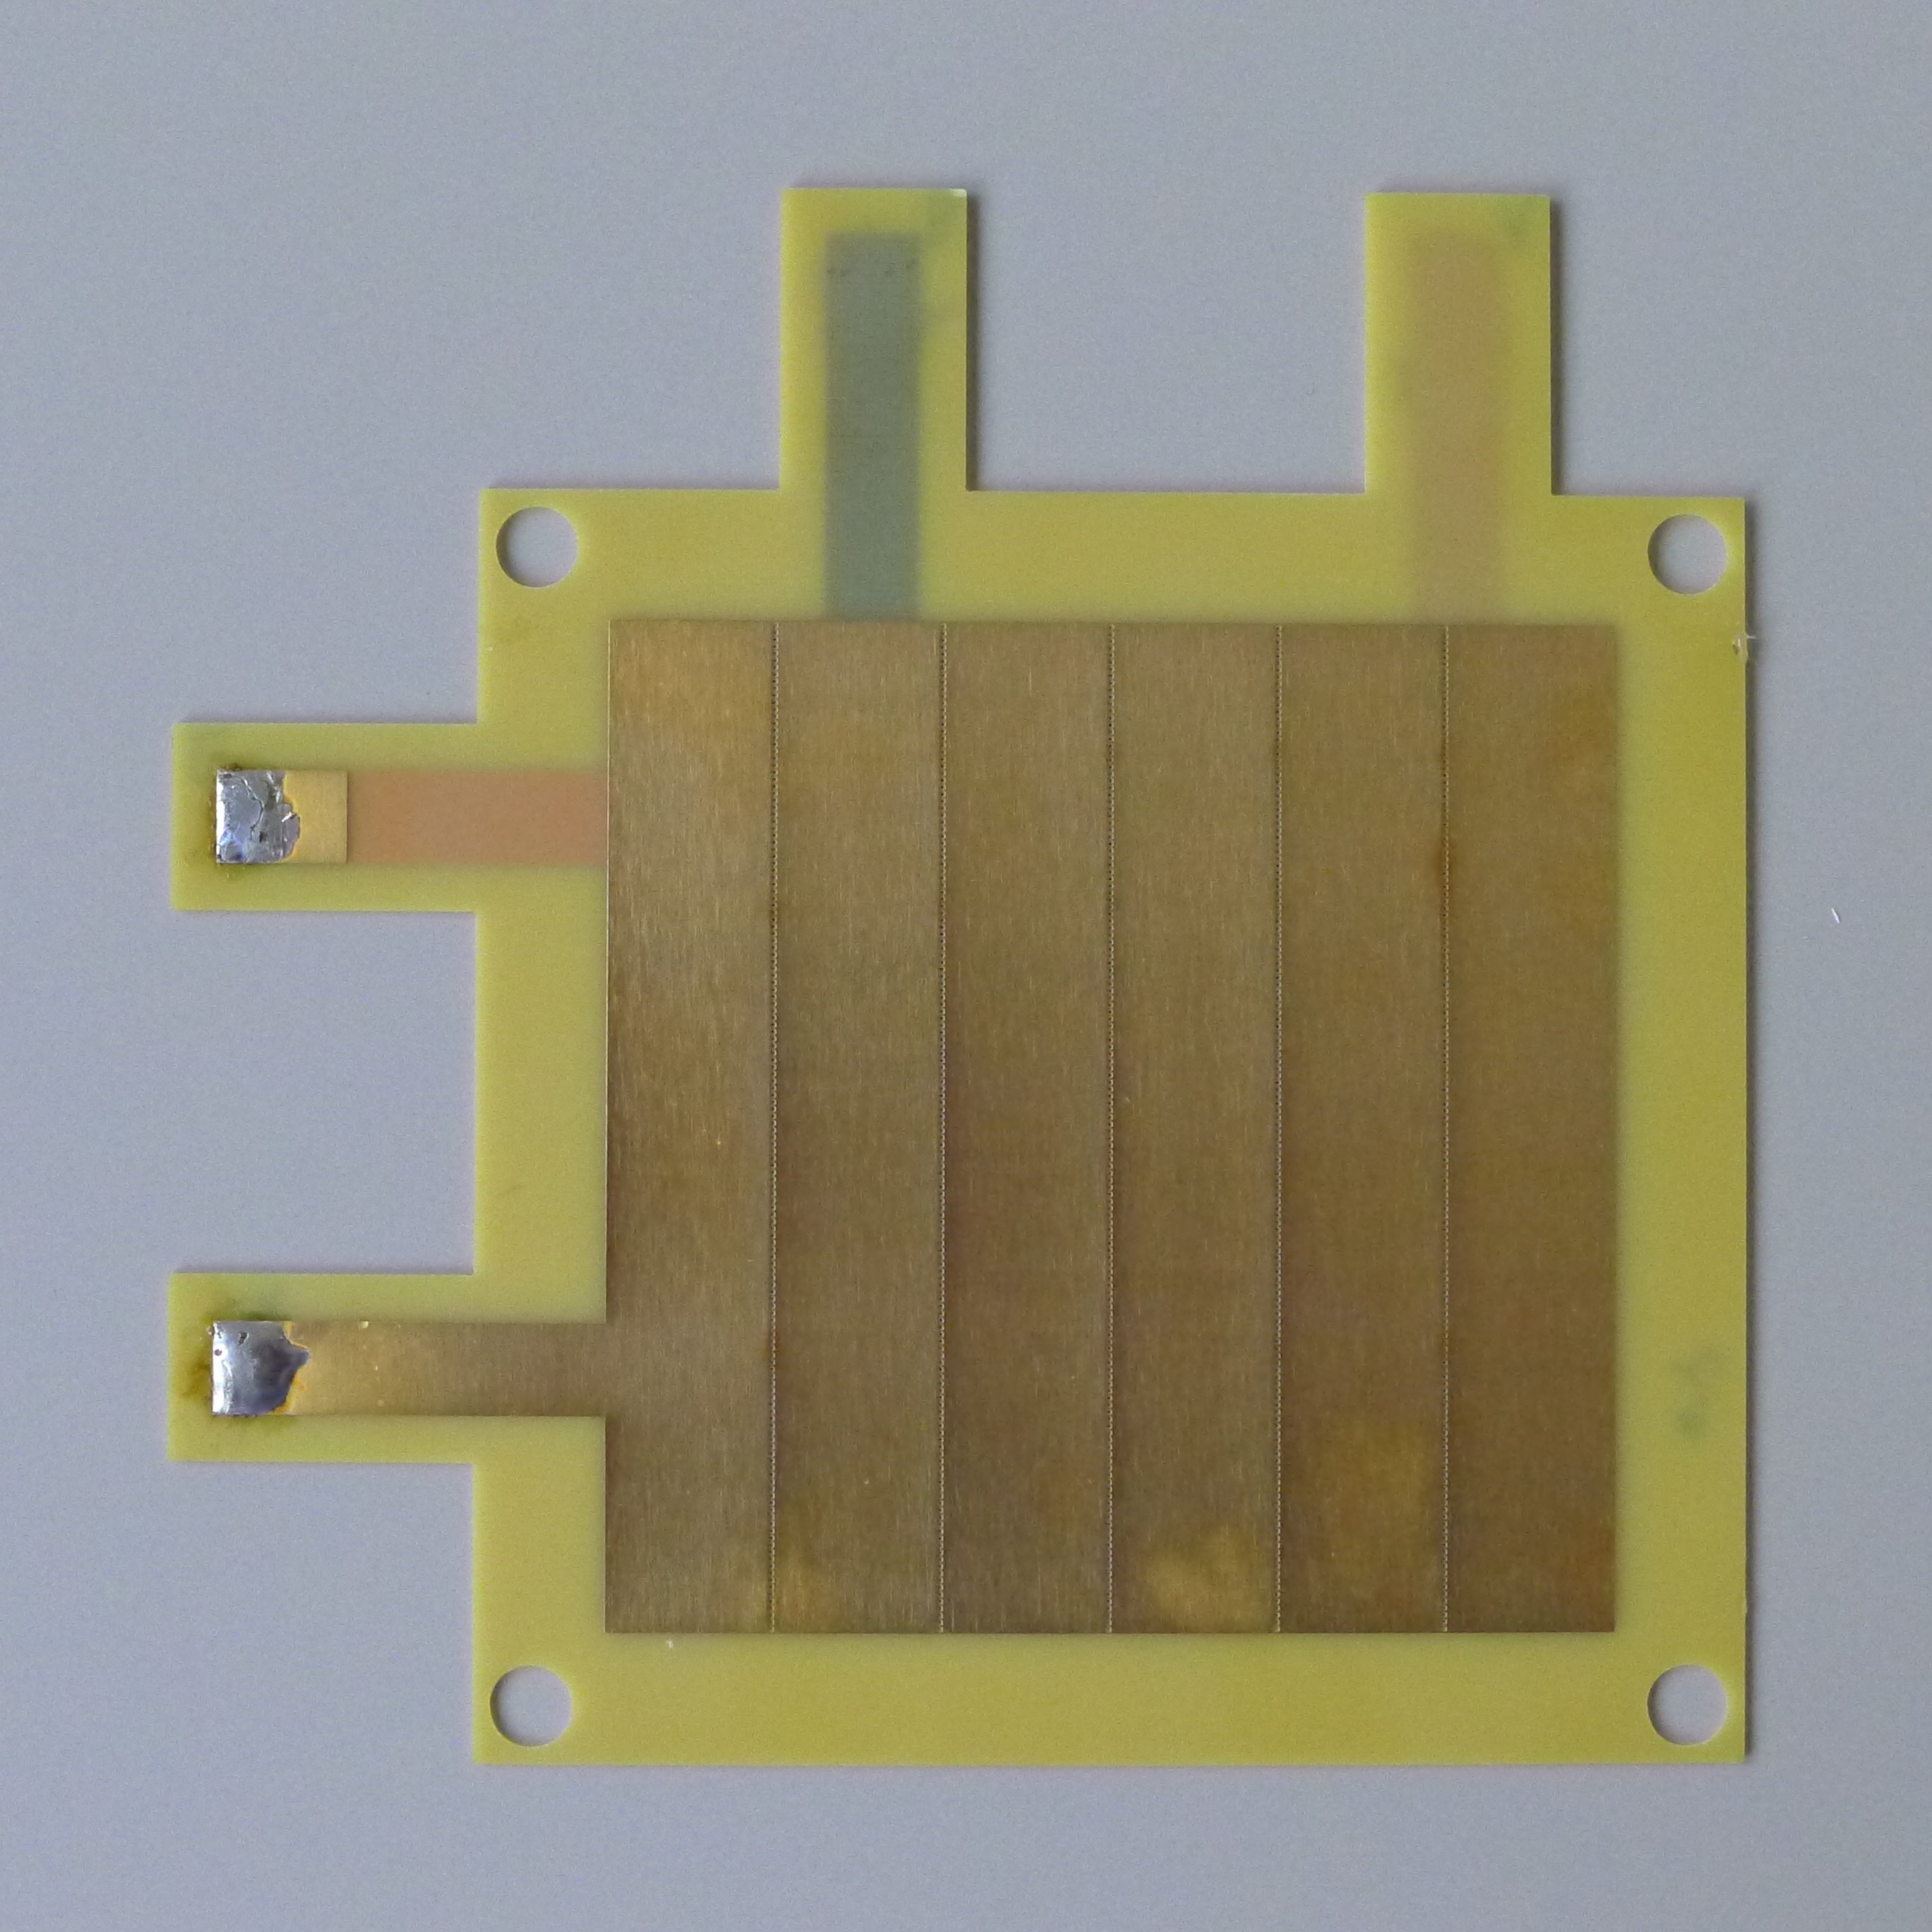
\includegraphics[width=0.45\textwidth]{Immagini/row_thgem.JPG}}
	\caption{Pictures of the FULL THGEM (a) and the ROW THGEM (b).}
%	\label{fig:full_thgem_complessiva}		
%\end{figure}
%\begin{figure}
%	\centering
	\subfigure[]{
	  \label{fig:row_thgem}
	  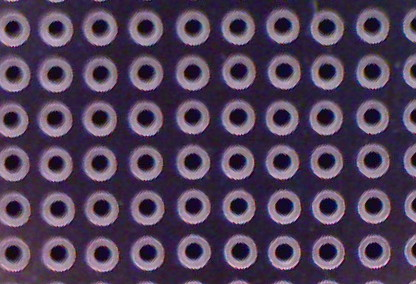
\includegraphics[width=0.45\textwidth]{Immagini/full_thgem_holes.JPG}}
	\hspace{5pt}
	\subfigure[]{
	 \label{fig:row_thgem_holes}
	 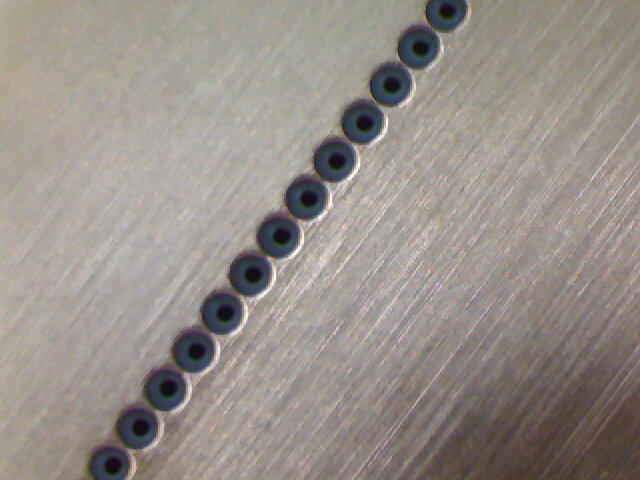
\includegraphics[width=0.45\textwidth]{Immagini/row_thgem_holes.JPG}}
	\caption{A magnification of the THGEM that show the different hole patterns: 
	(a) FULL THGEM, (b) ROW THGEM.}
	\label{fig:row_thgem_complessiva}		
\end{figure}

\subsection{The CAEN bias Supply and PICO}
\label{sec:bias}
The power supply of the prototype is based on a {\it Universal Multichannel Power Supply System 
SY5527LC}\footnote{https://www.caen.it/products/sy5527lc/} and an {\it Individual Floating Channel 
Dual Range Boards for Quadruple and Triple GEM detectors 
A1515}\footnote{https://www.caen.it/products/a1515/}. A scheme of the bias is shown in 
Fig.~\ref{fig:biasScheme1}. In Fig. \ref{fig:schema_apparato_2} a very simple scheme of the flows 
of positive ions and electrons is shown.
\begin{figure}[!htb]
	\centering
	\subfigure[]{ 
	 \label{fig:biasScheme1} 
	 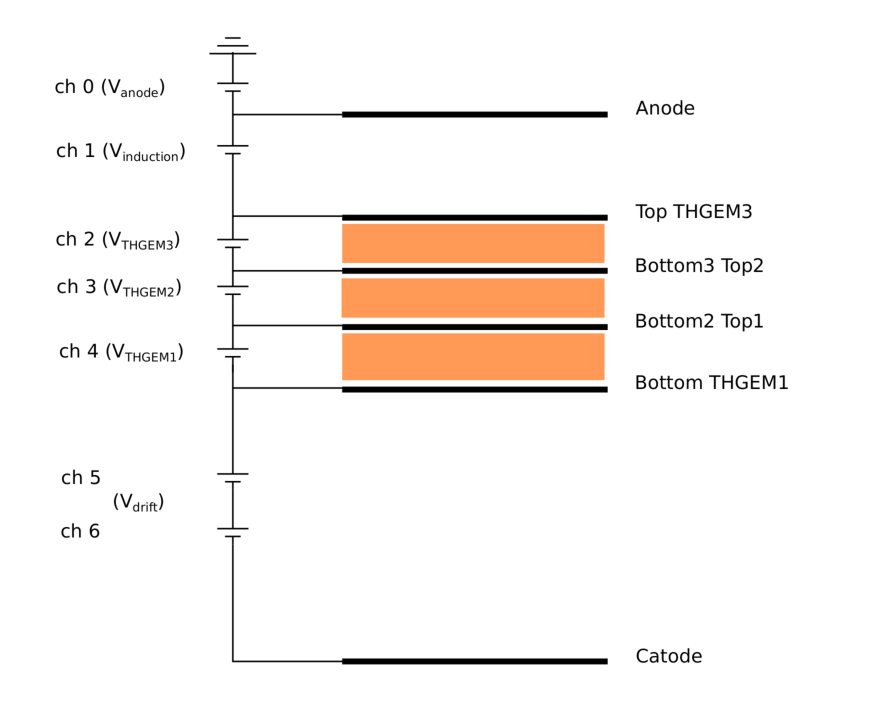
\includegraphics[width=0.8\textwidth]{Immagini/THGEM_Bias.pdf}}
	\subfigure[]{ 
	 \label{fig:biasScheme2} 
	 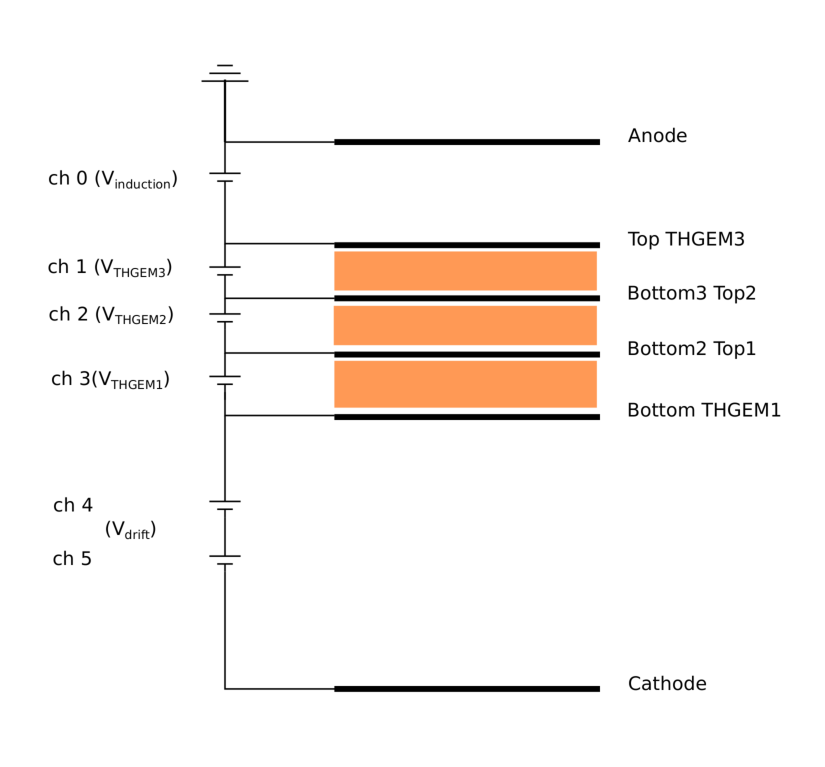
\includegraphics[width=0.8\textwidth]{Immagini/THGEM_Bias_2.pdf}}
	\caption{Scheme of the Bias supply during the meausurements with electronics a) and for the 
	 current measurements b).}
	\label{fig:induction_FULLTHGEM_other_pressure}
\end{figure}
The two ammeters: the CAEN ammeter integrated in the power supply (in the following just CAEN 
ammeter) and PICO do not measure exactly the same currents as illustrated in Fig. 
\ref{fig:run190_CAEN_pico}. In fact the 
CAEN ammeter measures the currents that flows in the branch where is the power supply while the 
PICO ammeter measures the current flowing in the branch where are the electrodes. The six measured
currents are: anode, top3, bot3/top2, bot2/top1, bot1 and cathode as shown in 
Figure~\ref{fig:schema_canali}. For the sake of clarity we underline that top 3 corresponds to the 
top layer of the 3-layers stack of THGEM, i.e. that one looking to the anode while bot 1 is the 
bottom layer of the stack, i.e. that one looking to the cathode. Bot3/top2 as well bot2/top1 
refers to the metallic layers embedded in the THGEM stack. In no case currents in these two 
electrodes have been observed.\\

The current read with PICO for bot 1 has usually a worse accuracy. This is due to the fact that 
PICO has two dynamical ranges with two related accuracy. Since in bot1 flow a large current due to 
the partition wires (see \ref{sec:prototype}) the dynamical range of PICO is the largest for such 
electrode and therefore the accuracy is worse\footnote{Also in cathode flows a current equal to 
bot1 but with an opposite charge but the two dynamical ranges are different for positive and 
negative currents. Therefore the current flowing in the bot1 is enough to switch the dynamical 
range for the bot1 channel but not enough to switch the dynamical range for the cathode channel.
This is why the bot 1 and cathode measure the same current in absolute value but have different
accuracies.}.
\begin{figure}
	\centering
	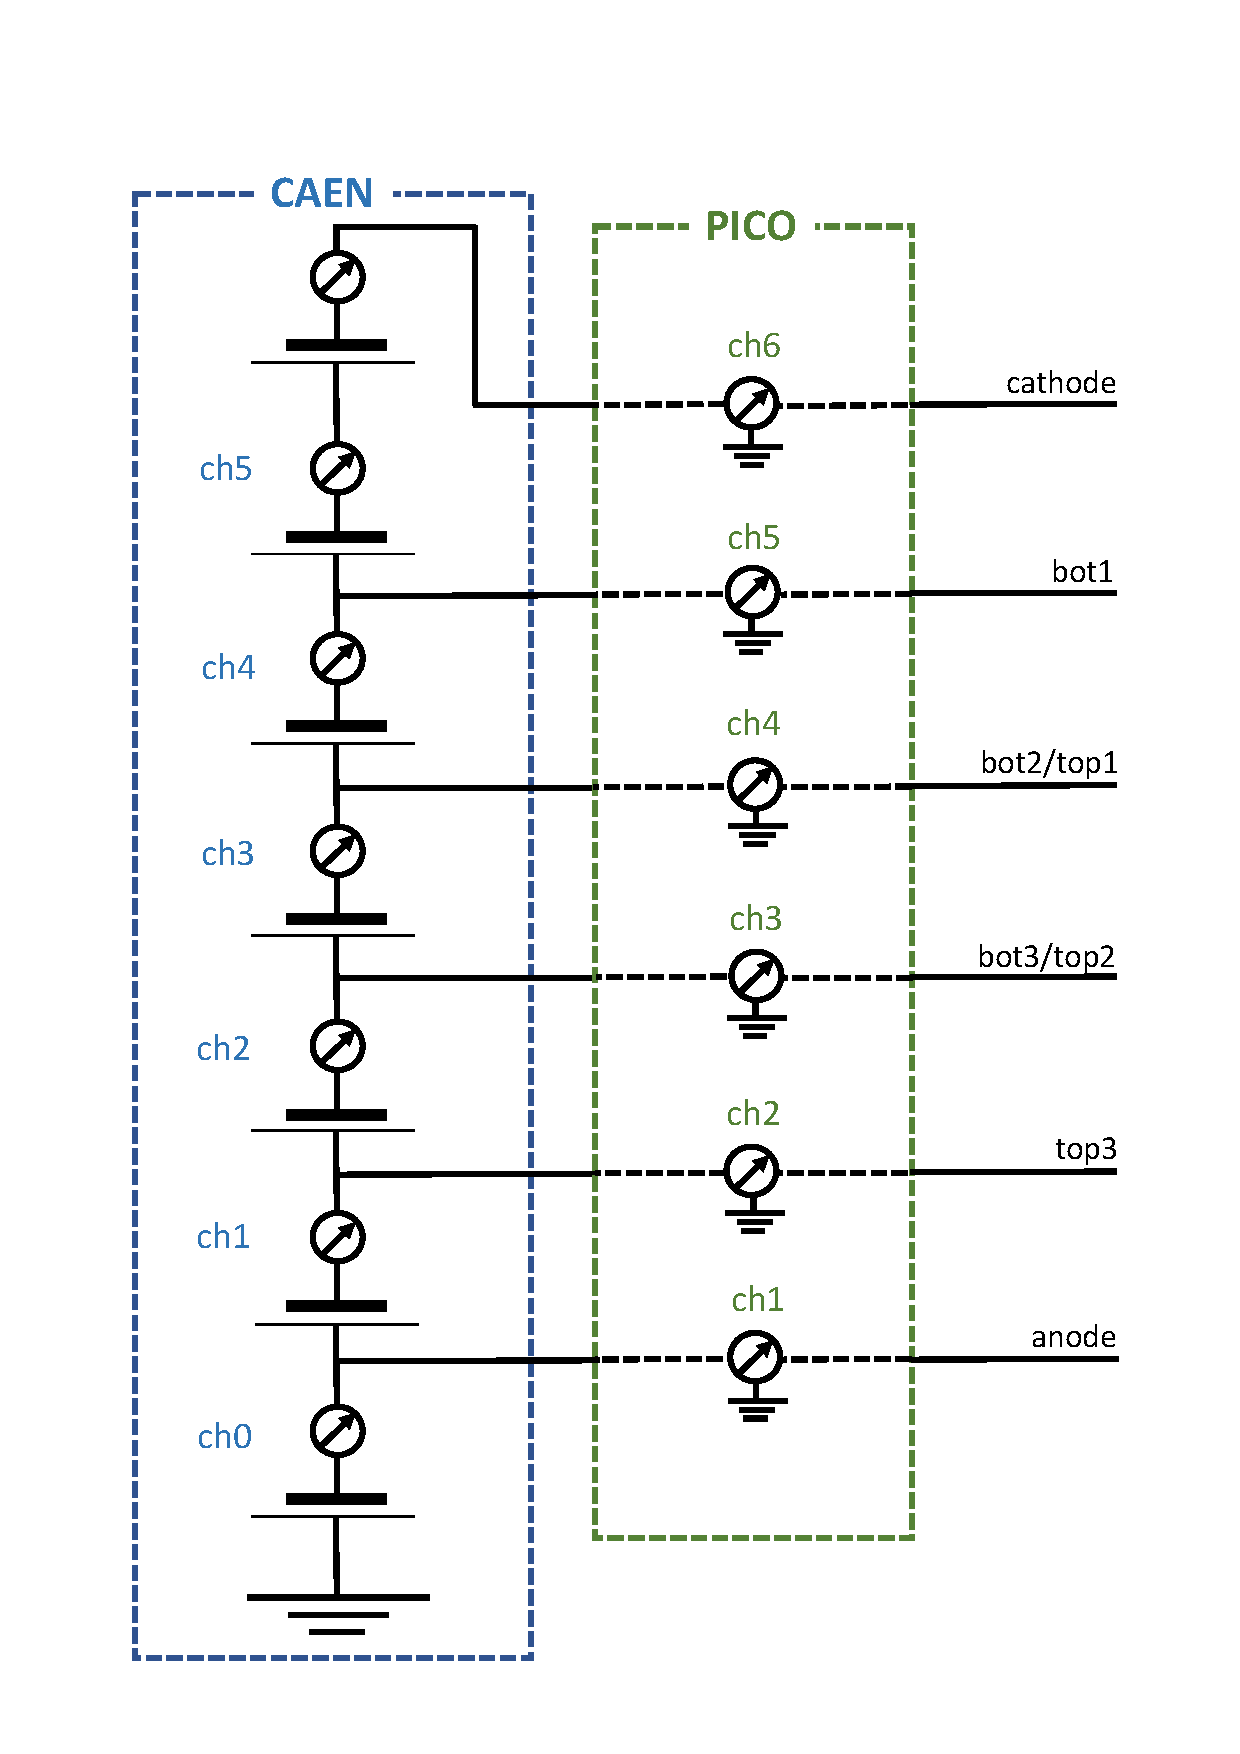
\includegraphics[width=0.5\textwidth]{Immagini/schema_canali_2.pdf}
	\caption{Current reading scheme for the two ammeters.}
	\label{fig:schema_canali}
\end{figure}
\begin{figure}
	\centering
	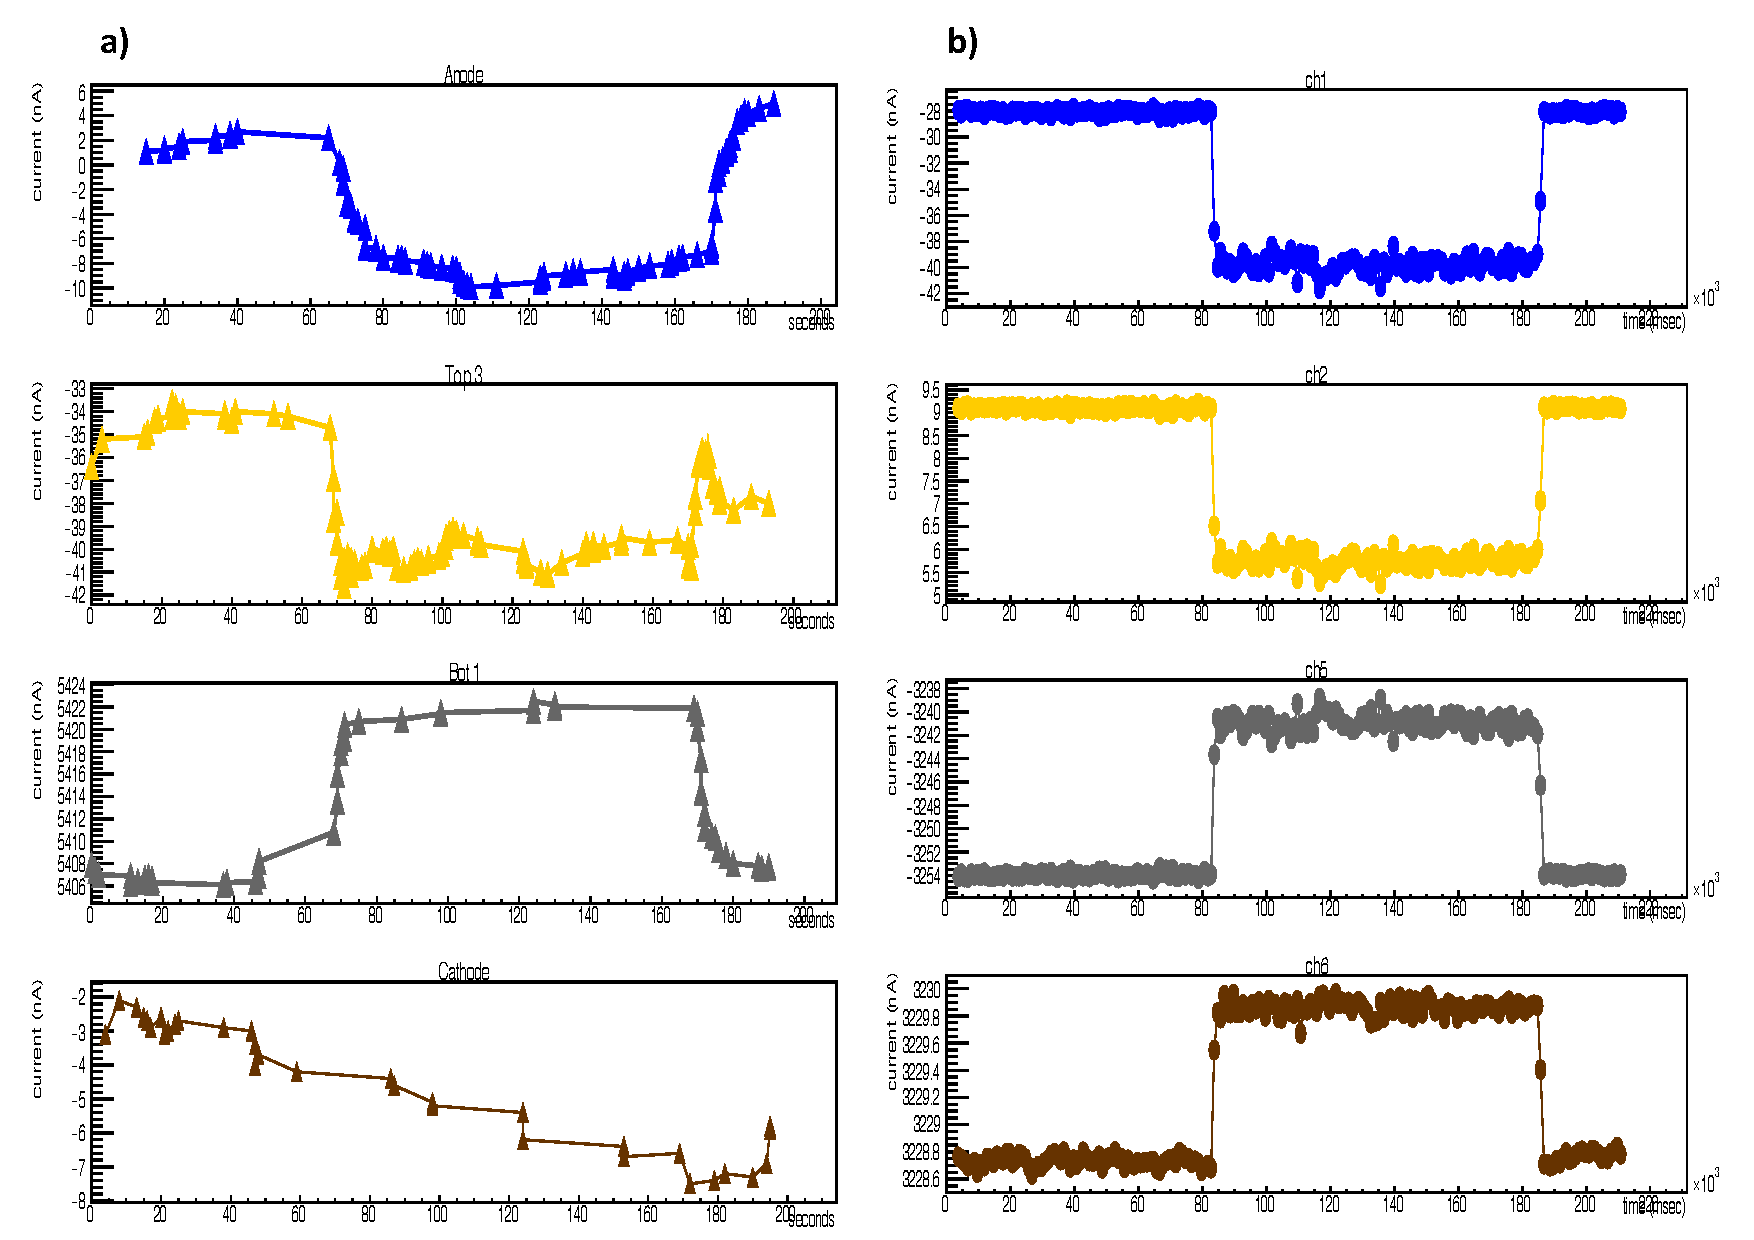
\includegraphics[width=0.7\textwidth]{Immagini/run190_CAEN_pico.pdf}
	\caption{Anode, Top3, Bot1 and Cathode currents measured with CAEN ammeter a) and PICO b).}
	\label{fig:run190_CAEN_pico}
\end{figure}

\section{Method}

The main parameters that determine the behaviour of the detector are: gas pressure, voltage of the 
THGEM (V$_{THGEM}$), voltage of the induction region (V$_{ind}$) and voltage of the drift region 
(V$_{drift}$).
The cathode cannot be kept connectd at ground if we want to measire the current flowing on it,
therefore the anode was kept at voltage fixed to an arbitrary value of 20~V (see Fig. 
\ref{Immagini/THGEM_Bias_2.pdf}). This value should not affect the measurements of the currents of 
any electrodes.\\

The method consists in keeping fix all the parameter but one and to measure all the currents of 
all the electrodes varying just the parameters let free to change. For example we keep fix the gas 
pressure the V$_{drift}$, V$_{ind}$, while the V$_{THGEM}$ was changed a small step. In this way 
we get 6 plots as a function of V$_{THGEM}$, one for each current i.e. anode, bot1, bot2/top1, 
bot3/top2, top3 and cathode.
%For example, during the $\Delta V_{ind}$ scan, the $\Delta V_{THGEM}$ and $\Delta_{drift}$ were 
%fixed and anode, bot1, top3 and cathode currents were measured (see 
%Figure~\ref{fig:schema_canali}).\\
A run lasts usually 180 s (see Fig. \ref{fig:run190_CAEN_pico}):\\
60 s with shutter closed;\\
90 s with shutter open;\\
30 s with shutter closed.\\
An average of the current flowing during the first 60 s (shutter closed) and an average during
the 90 s with shutter open is performed. The difference between the two measurements with shutter 
open and closed gives the actual current associated to the $\alpha$-particles entering the 
detector. In this way any dark current coming from the detector or from the ammeter is 
subtracted\footnote{A possible source of dark current is due to the X-ray produced by the 
$\alpha$-source that are not stopped by the shutter.}.\\

In Figure~\ref{fig:run190_CAEN_pico} a comparison of the same run measured using the two 
ammeters is shown. It is eveident the better accuracy of PICO.

\clearpage

\chapter{Measurements}
%i canali 3 e 4 possono essere ignorati perche non danno mai segnale

%spieghiamo i diversi scan (induzione, thgem e drift)

This section contain a description of the current measurements that was performed. It  is
organized as follow. First are presented the measurements with the Full THGEM and after those with 
the Row THGEM. For each THGEM are presented in the following order the scan of the induction The 
scan of the THGEM and eventually the scan of the Drift.\\
A separate section is devoted to the study of the in-beam test.

\section{test with $\alpha$-source}

\subsection{FULL THGEM}
The FULL THGEM was made by the xxx manufacturer. Their characterstics are summarized in Tab.
\ref{tab:thgem}.

\subsubsection{Scan on \Vind}
In this subsection a series of systematic measurements were performed to study the effects of the 
variation of the voltage \Vind{} on all the measured currents. These measurements were 
done at different pressures (P) and values of \Vthgem{} and \Vdrift{}, a summary scheme of the 
configurations is shown in Table~\ref{tab:FULLTHGEM_vind}.
\begin{table} [b!]
	\begin{center}
		\renewcommand{\arraystretch}{1.2}
		\begin{tabular} {ccccccc}
			P (mbar) & & \Vthgem{} (V) & & \Vdrift{} (V) & & \\
			\toprule[0.1em]
			%\hline
			30.2	& &	220	& &	1000 & & 5-28 \\
			30.4	& &	200	& &	1000 & & 61-75\\
			30.4	& &	230	& &	1000 & & 76-89\\
			20.5	& &	200	& & 1000 & & 90-111\\
			11	    & & 170	& & 600 & & 146-168\\
     		\bottomrule[0.1em]
		\end{tabular}
	\end{center}
	\caption{The values of pressure (P), \Vthgem{} and \Vdrift{} adopted for the study on \Vind.} 
	\label{tab:FULLTHGEM_vind}
\end{table}
The \Vind{} scans were carried out starting from 0~V and increasing the voltage by 10 or 20~V per run, 
until the discharge value is reached.
This value is dependent on the gas pressure and possibly on the values set for \Vthgem{} and \Vdrift.
The values at which discharge occurs are 220, 200 and 150 V for 30, 20 and 11 mbar respectively.\\

A typical example of the scan is shown in Figure~\ref{fig:induction_FULLTHGEM_30mbar}, it corresponds
at 30~mbar and \Vthgem{}~=~220~V. By raising the value of \Vind{}, the anodic current (blue line) 
increases, while the top3 current (yellow line) decreases approaching zero.
\begin{figure}[!t]
	\centering
	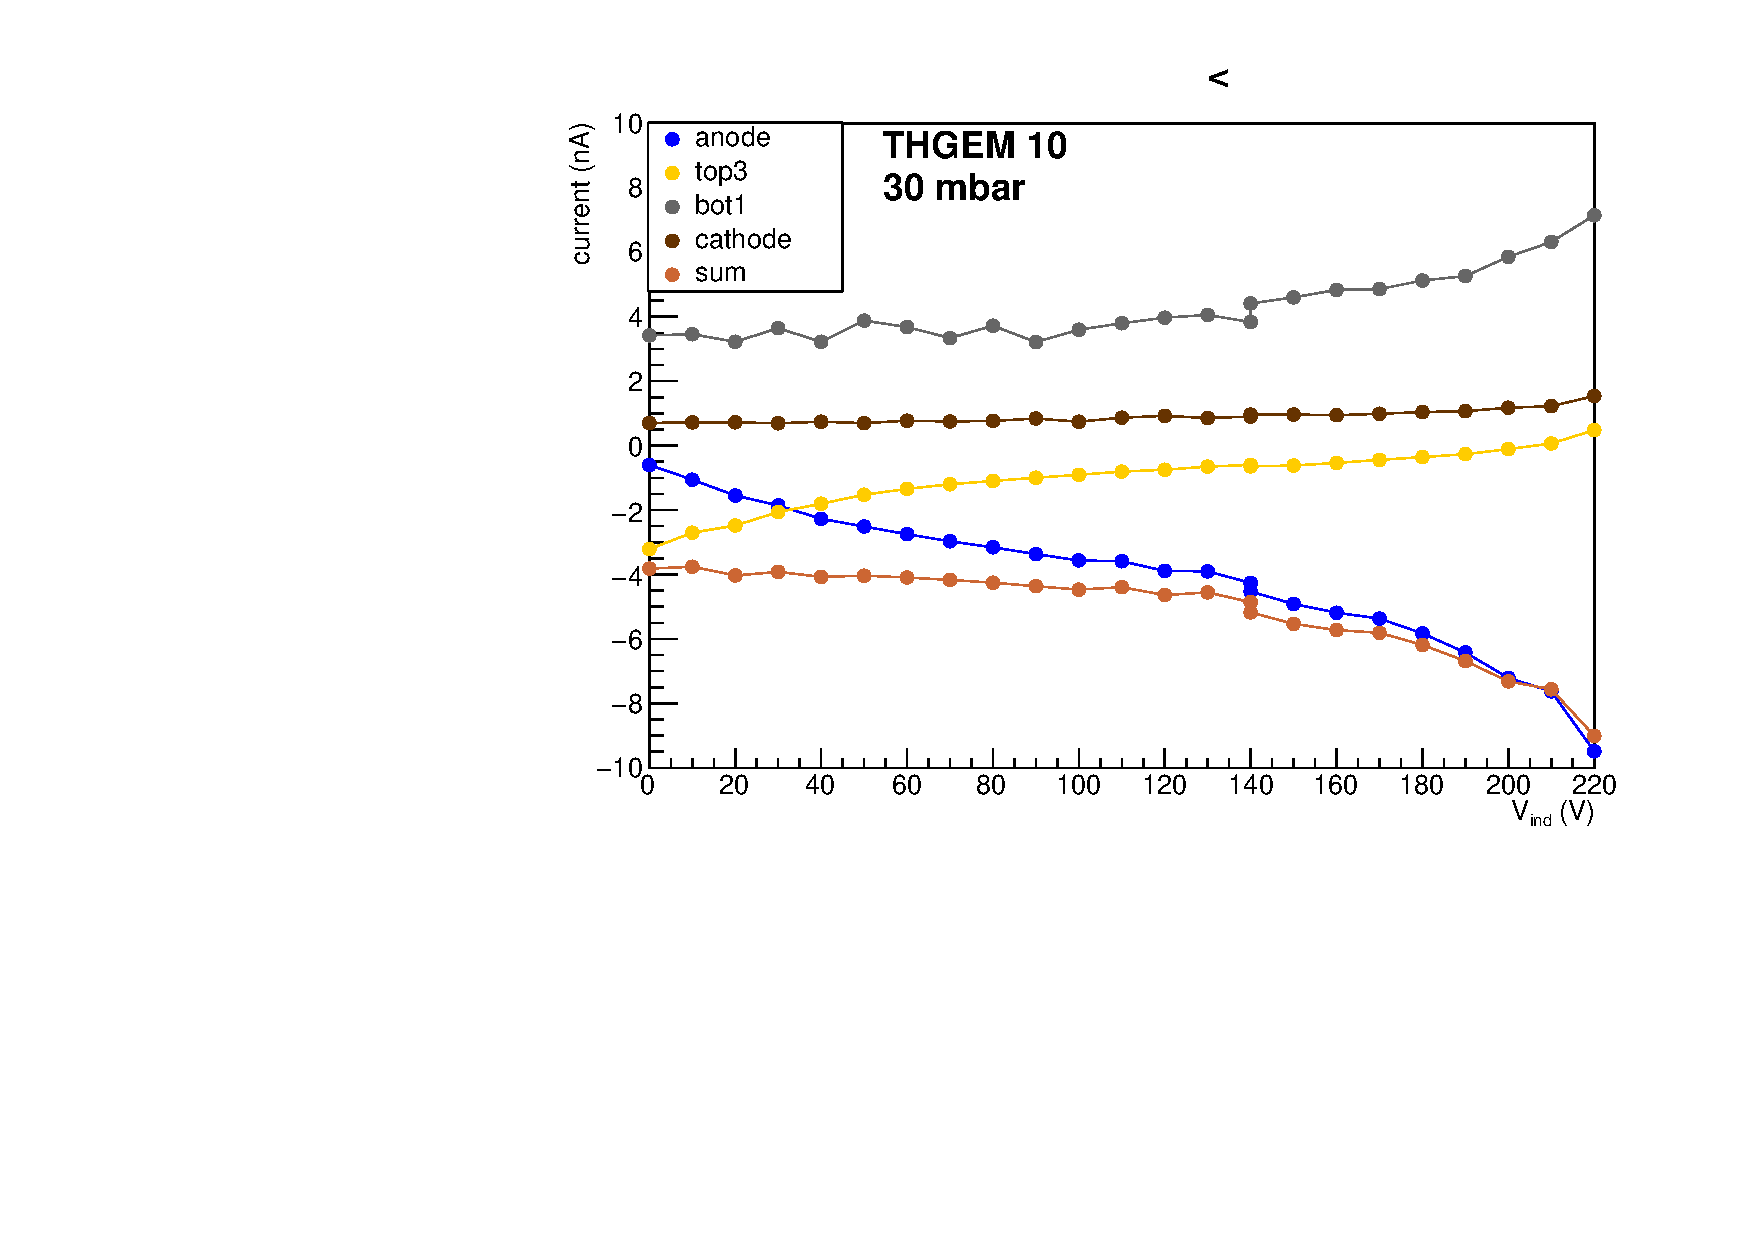
\includegraphics[width=\textwidth]{Immagini/inductionScan_THGEM10_30mbar.pdf}
	\caption{Currents measured during the scan on the voltage \Vind{} across the induction region at 
	30~mbar and with \Vthgem{}~=~220~V.}
	\label{fig:induction_FULLTHGEM_30mbar}
\end{figure}
The orange points corresponds to the sum of the currents read in top3 and anode, that is to the total 
negative charge (TNC) produced by the THGEM. Up to 140~V, The TNC is approximately constant, 
for values higher than 140 V the TNC increases.
This simply means that the stronger is the electric field in the induction region, the greater is 
the fraction of secondary electrons collected at the anode and lower is the fraction of the 
electrones collected by the top3 electrode.
For \Vind{} greater than 140~V, the TNC increases: this behaviour can be explained assuming that, 
when the voltage is high enough, the multiplication region extends out of the THGEM holes, 
expanding in the induction region (see Fig.~\ref{fig:induction_FULLTHGEM_30mbar_other_VTHGEM} for a 
more evident effect.). For values of \Vind{} still higher, the top3 current becomes positive (see 
Fig.~\ref{fig:induction_FULLTHGEM_other_pressure} b)). That is, a fraction of the positive ions 
produced in the induction region is cannot flow through the THGEM holes instead is directly 
collected by the top3 electrode.\\

An operational value of \Vind{}=120~V have been choosen, this value ensure that a large fraction of 
the electron is collected on the anode and that the multiplication is mainly confined on the THGEM 
holes.

The scan was repeated for two different values of \Vthgem{}: namely 200 and 230 V 
%(see Fig~\ref{fig:induction_FULLTHGEM_30mbar_other_VTHGEM}) 
and for two different pressures 10 and 20 mbar 
Fig.~\ref{fig:induction_FULLTHGEM_other_pressure}. In all cases the behaviour of the
curves is the same.

\begin{figure}[!htb]
	\centering
	\subfigure[]{ 
	  \label{fig:induction_FULLTHGEM_30mbar_other_VTHGEM_a} 
	  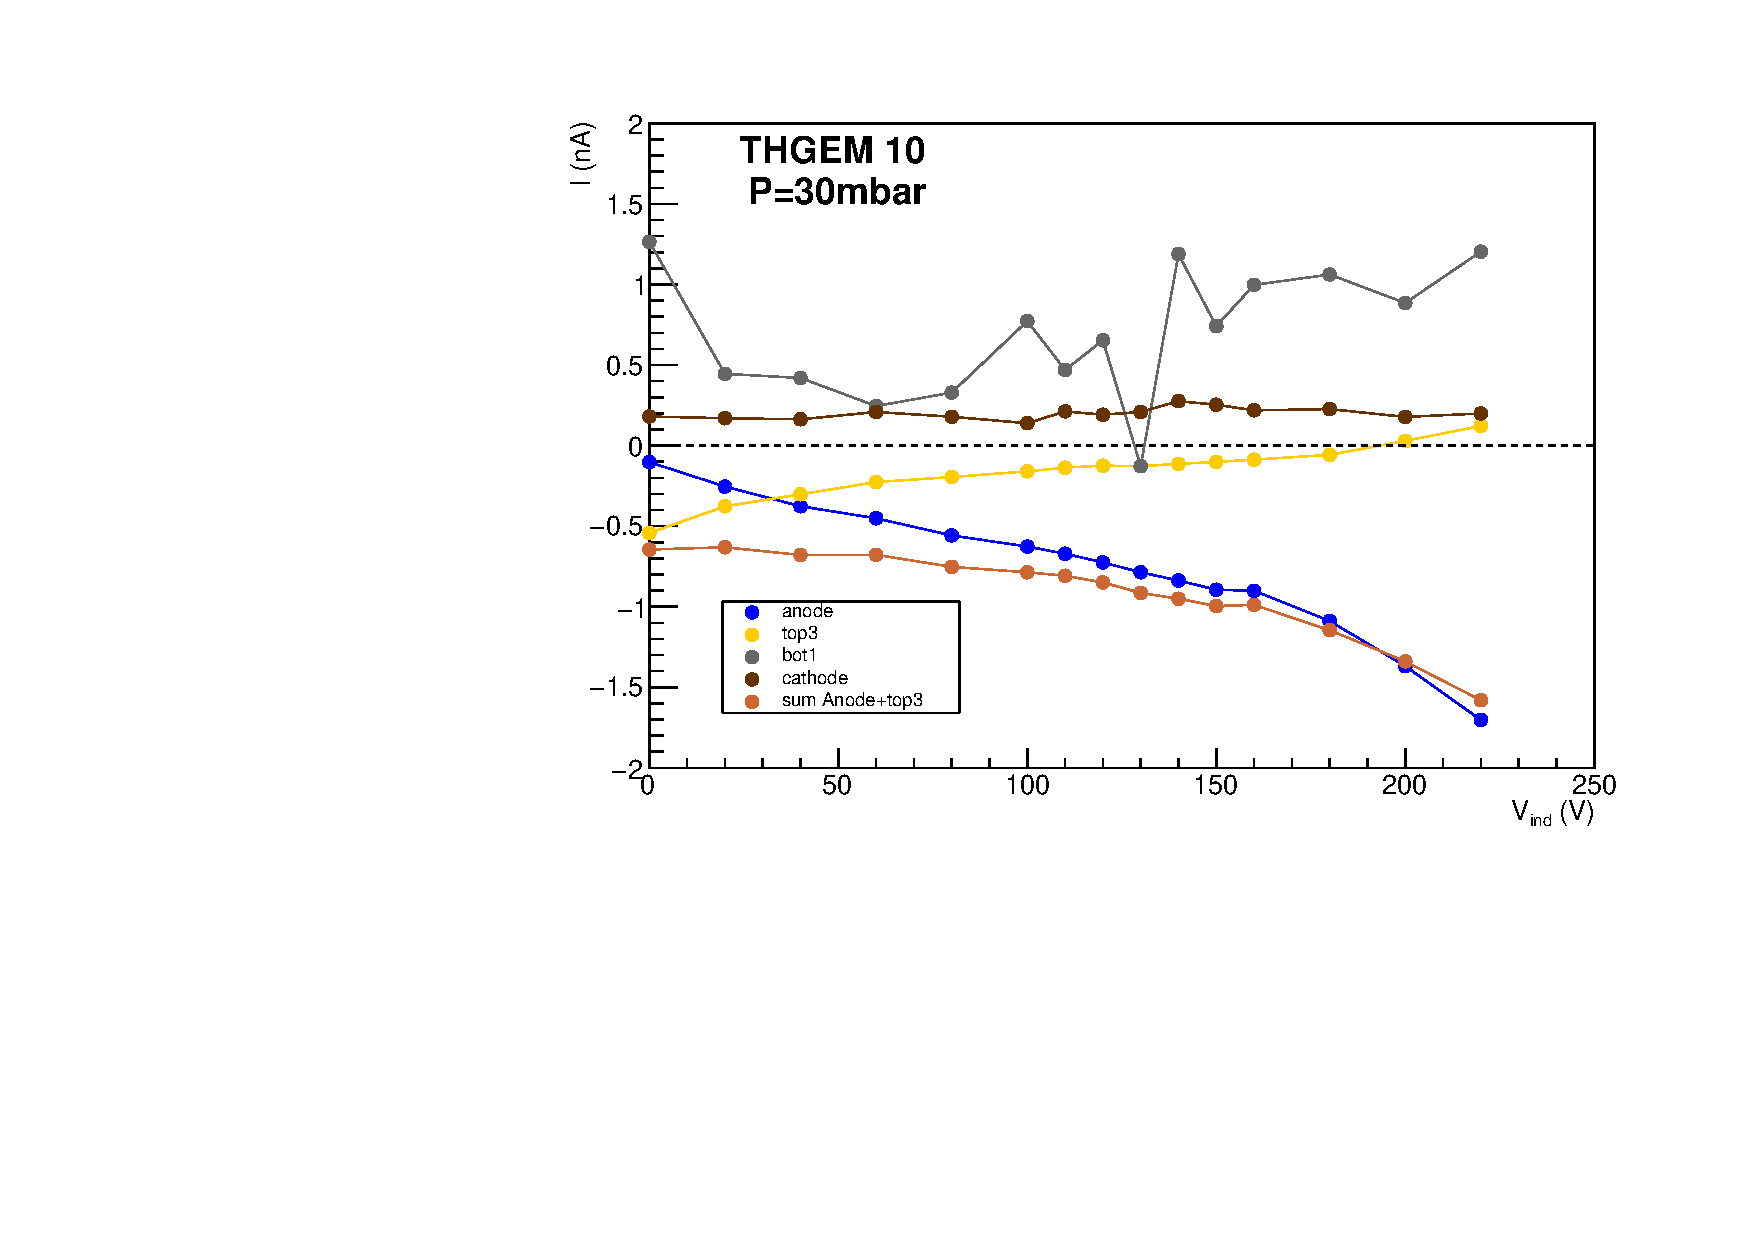
\includegraphics[width=0.96\textwidth]{Immagini/inductionScan_THGEM10_30mbar_bis.pdf}}
	\subfigure[]{ 	
	  \label{fig:induction_FULLTHGEM_30mbar_other_VTHGEM_b} 
	  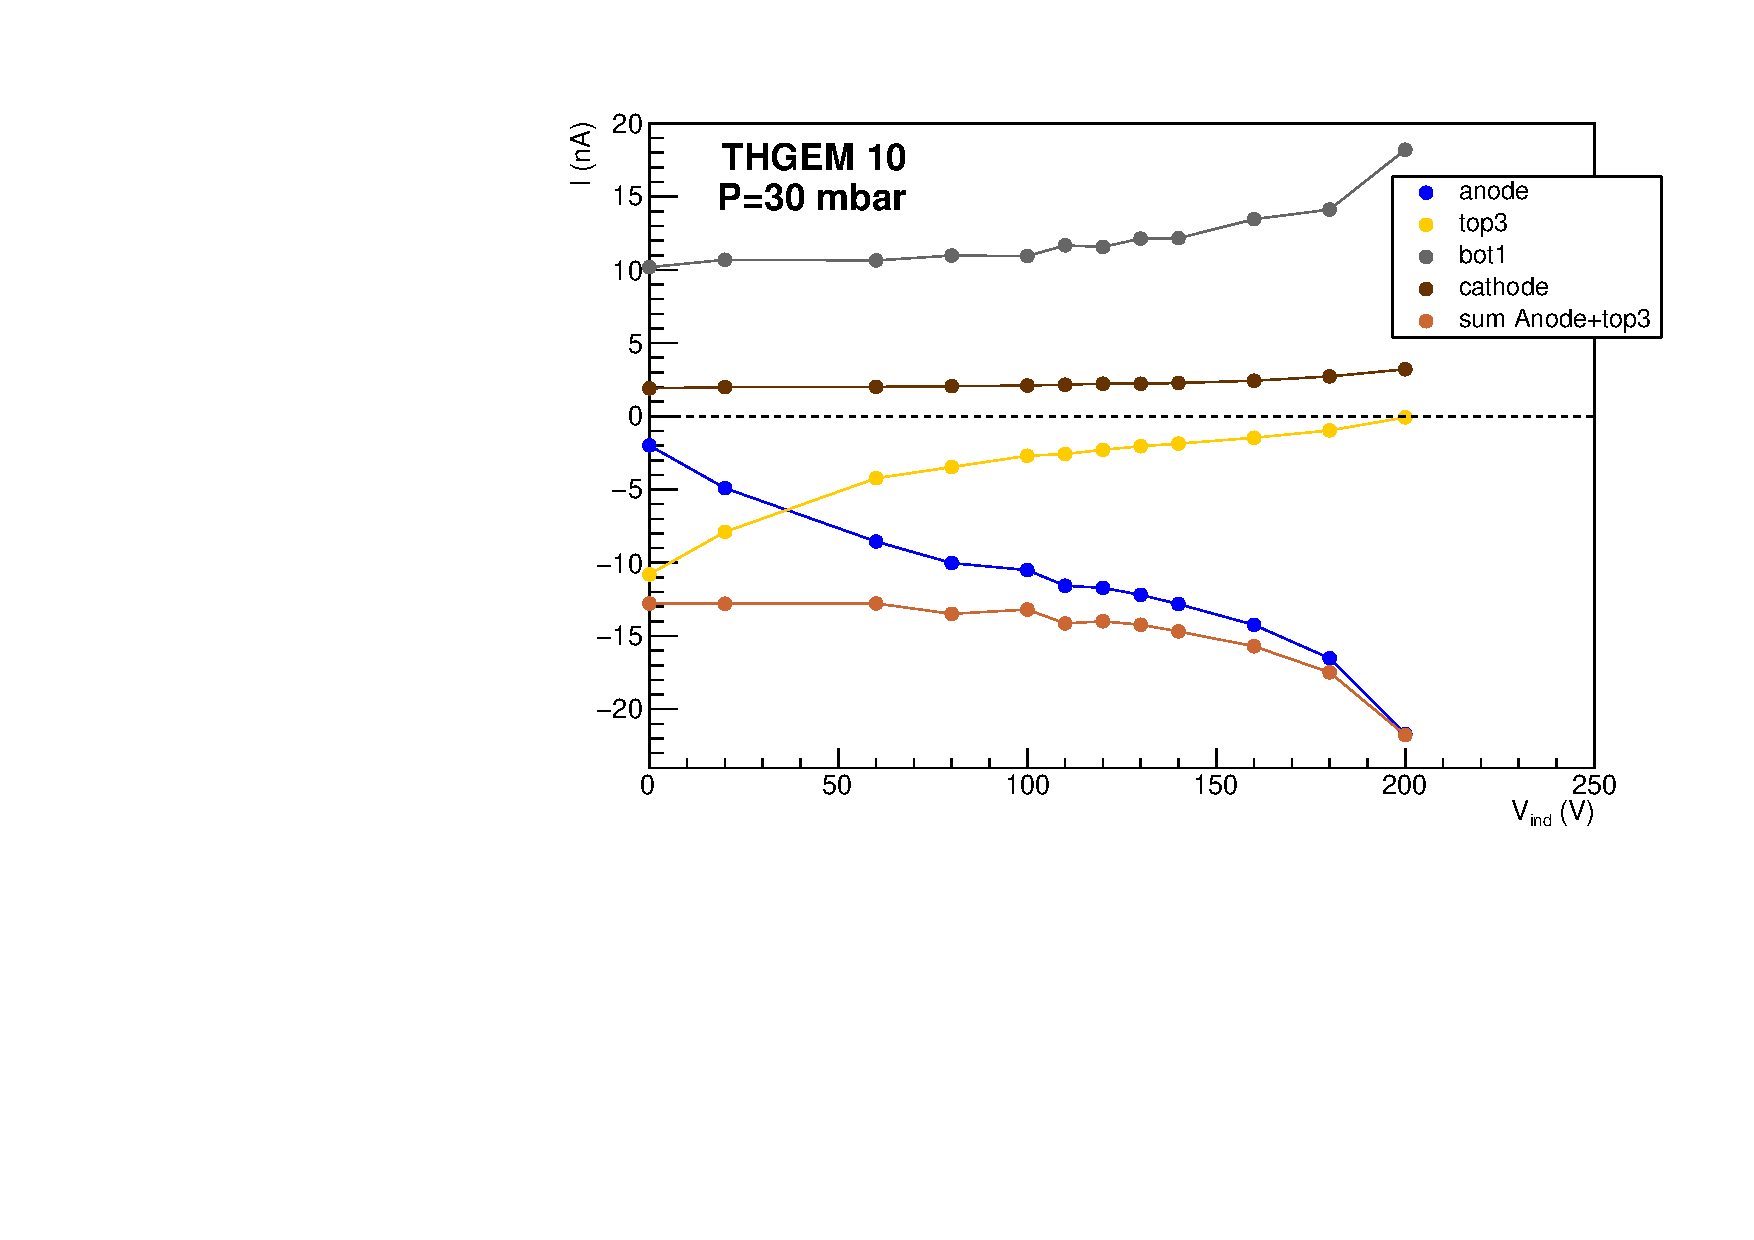
\includegraphics[width=0.96\textwidth]{Immagini/inductionScan_THGEM10_30mbar_tris.pdf}}
	\caption{Currents measured during the scan on the voltage \Vind{} across the induction region at 
	  30~mbar: in (a) for \Vthgem~=~200~V, in (b) for \Vthgem~=~230~V. In a) the bot1 current 
	  fluctuations are due to the lower accuracy of the corresponding PICO channel.}
	\label{fig:induction_FULLTHGEM_30mbar_other_VTHGEM}
\end{figure}

%\begin{figure}[!htb]
%	\centering
%	\subfigure[]{ 
%	  \label{fig:induction_FULLTHGEM_20mbar} 
%	  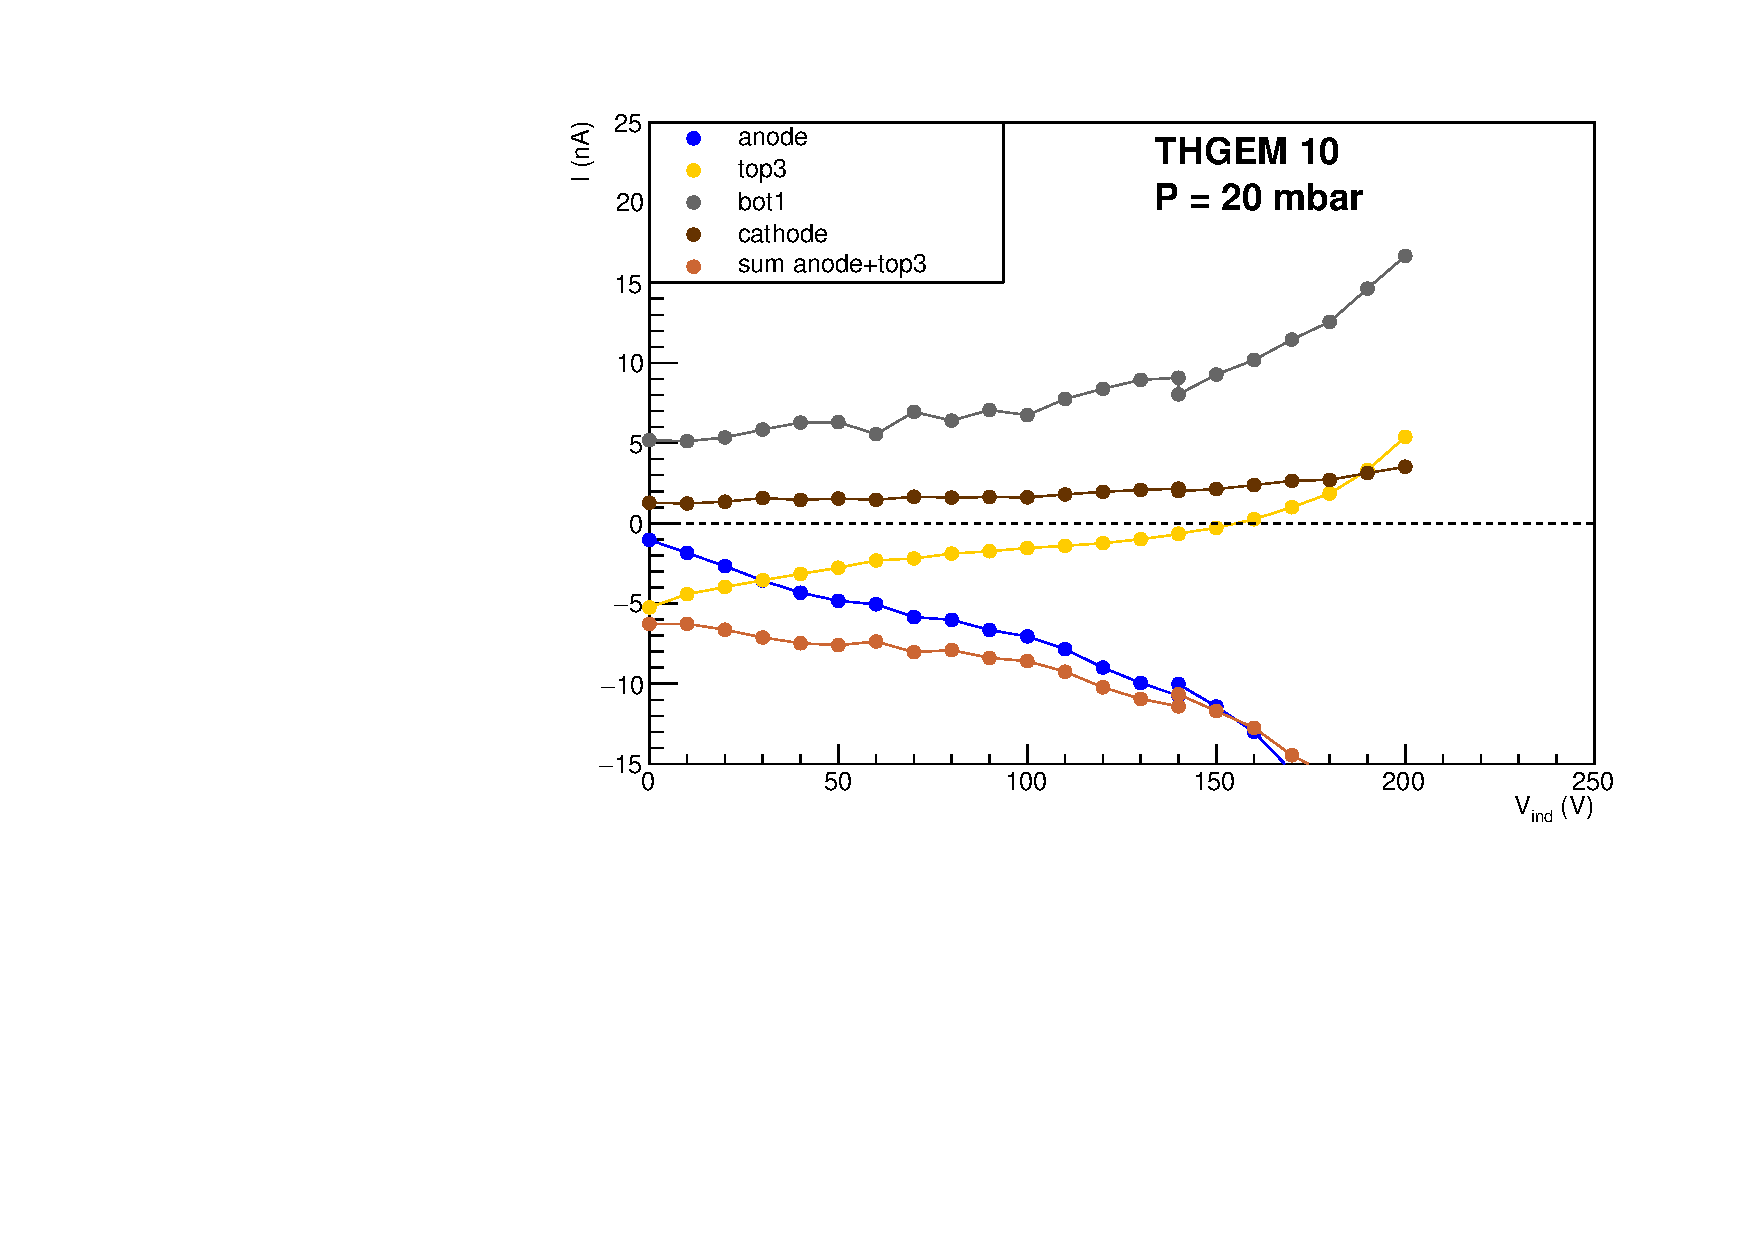
\includegraphics[width=0.97\textwidth]{Immagini/inductionScan_THGEM10_20mbar.pdf}}
%	\subfigure[]{ 
%	  \label{fig:induction_FULLTHGEM_11mbar} 
%	  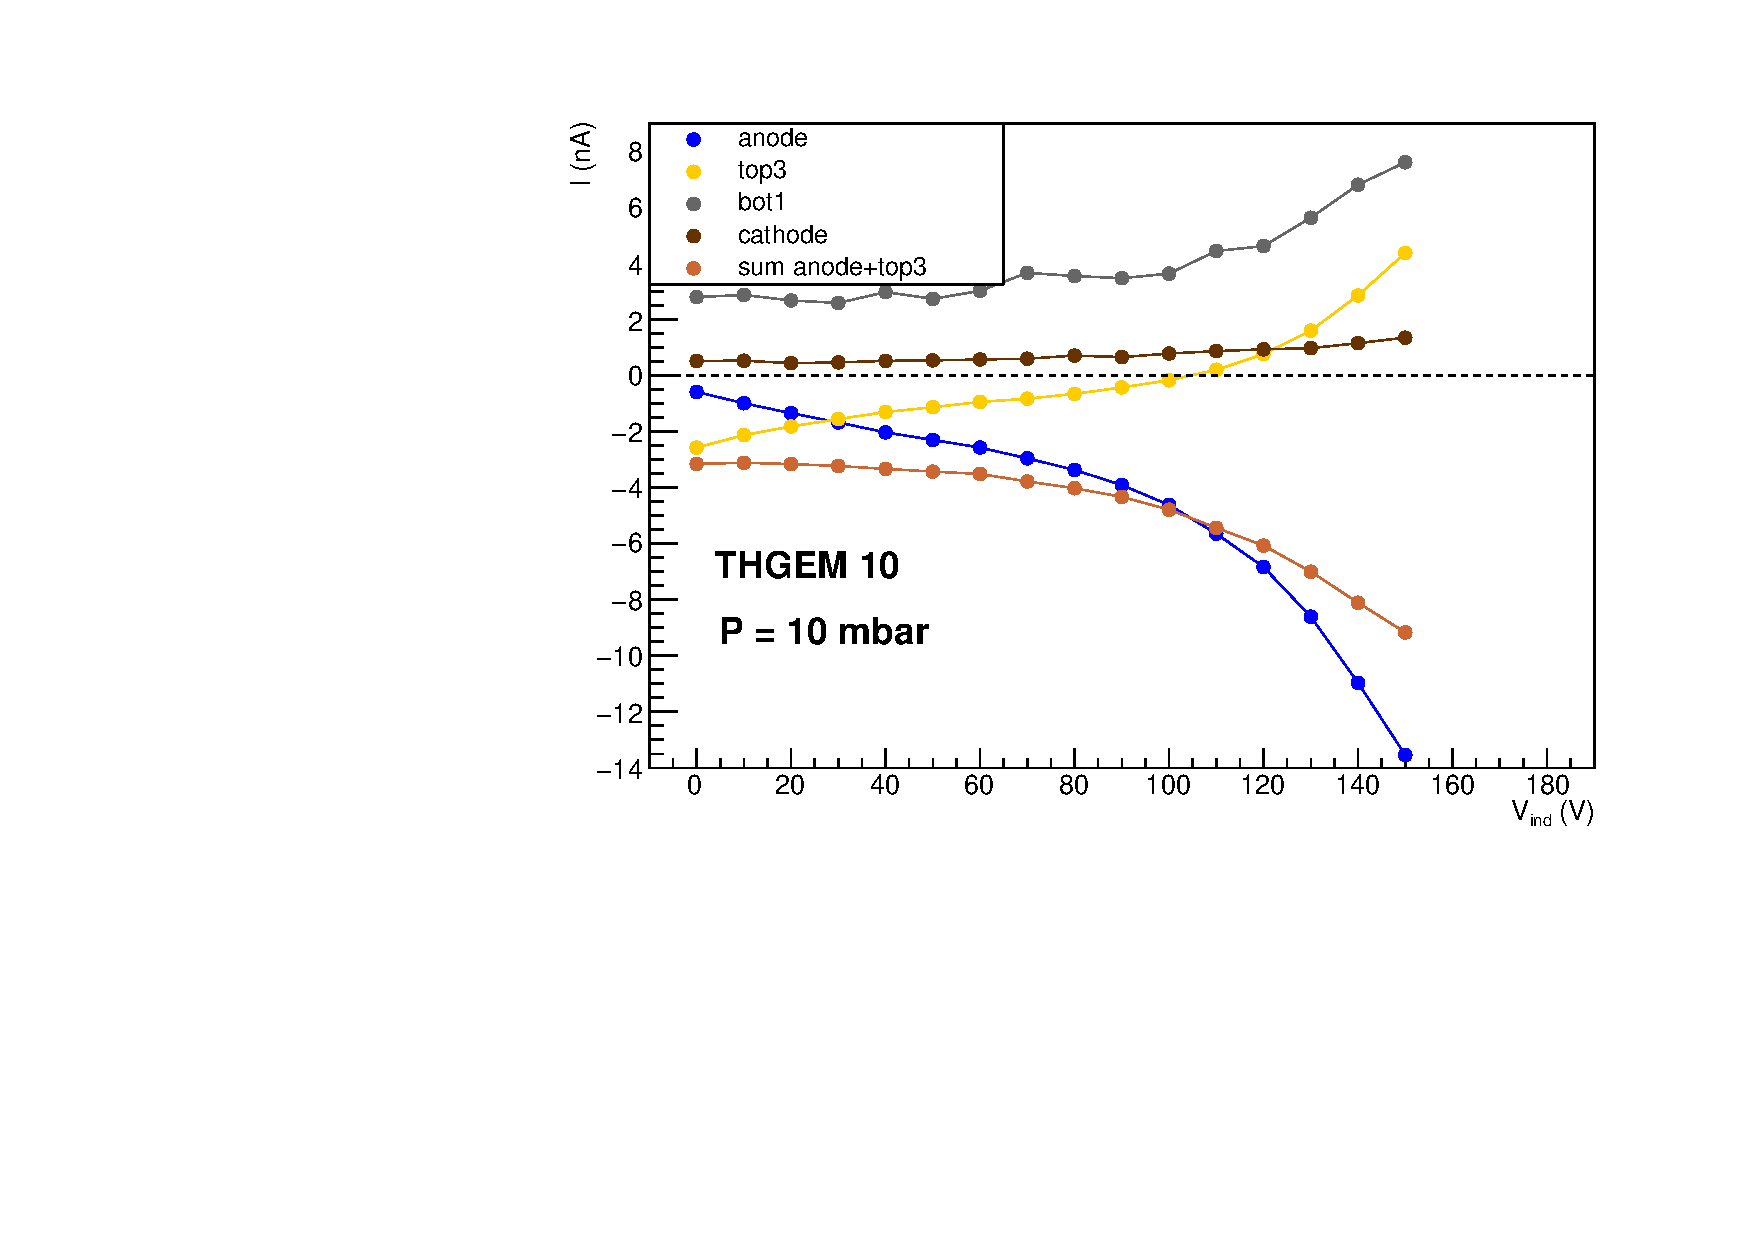
\includegraphics[width=0.97\textwidth]{Immagini/InductionScan_THGEM10_10mbar_tris.pdf}}
%	\caption{Currents measured during the scan on the voltage \Vind{} across the induction region: in 
%	(a) at 20~mbar, in (b) at 11~mbar.}
%	\label{fig:induction_FULLTHGEM_other_pressure}
%\end{figure}

A comparison of anode and top3 current at three different pressures are shown in Fig. 
\ref{fig:induction_pressure_comp}.
\begin{figure}[!htb]
	\centering
	  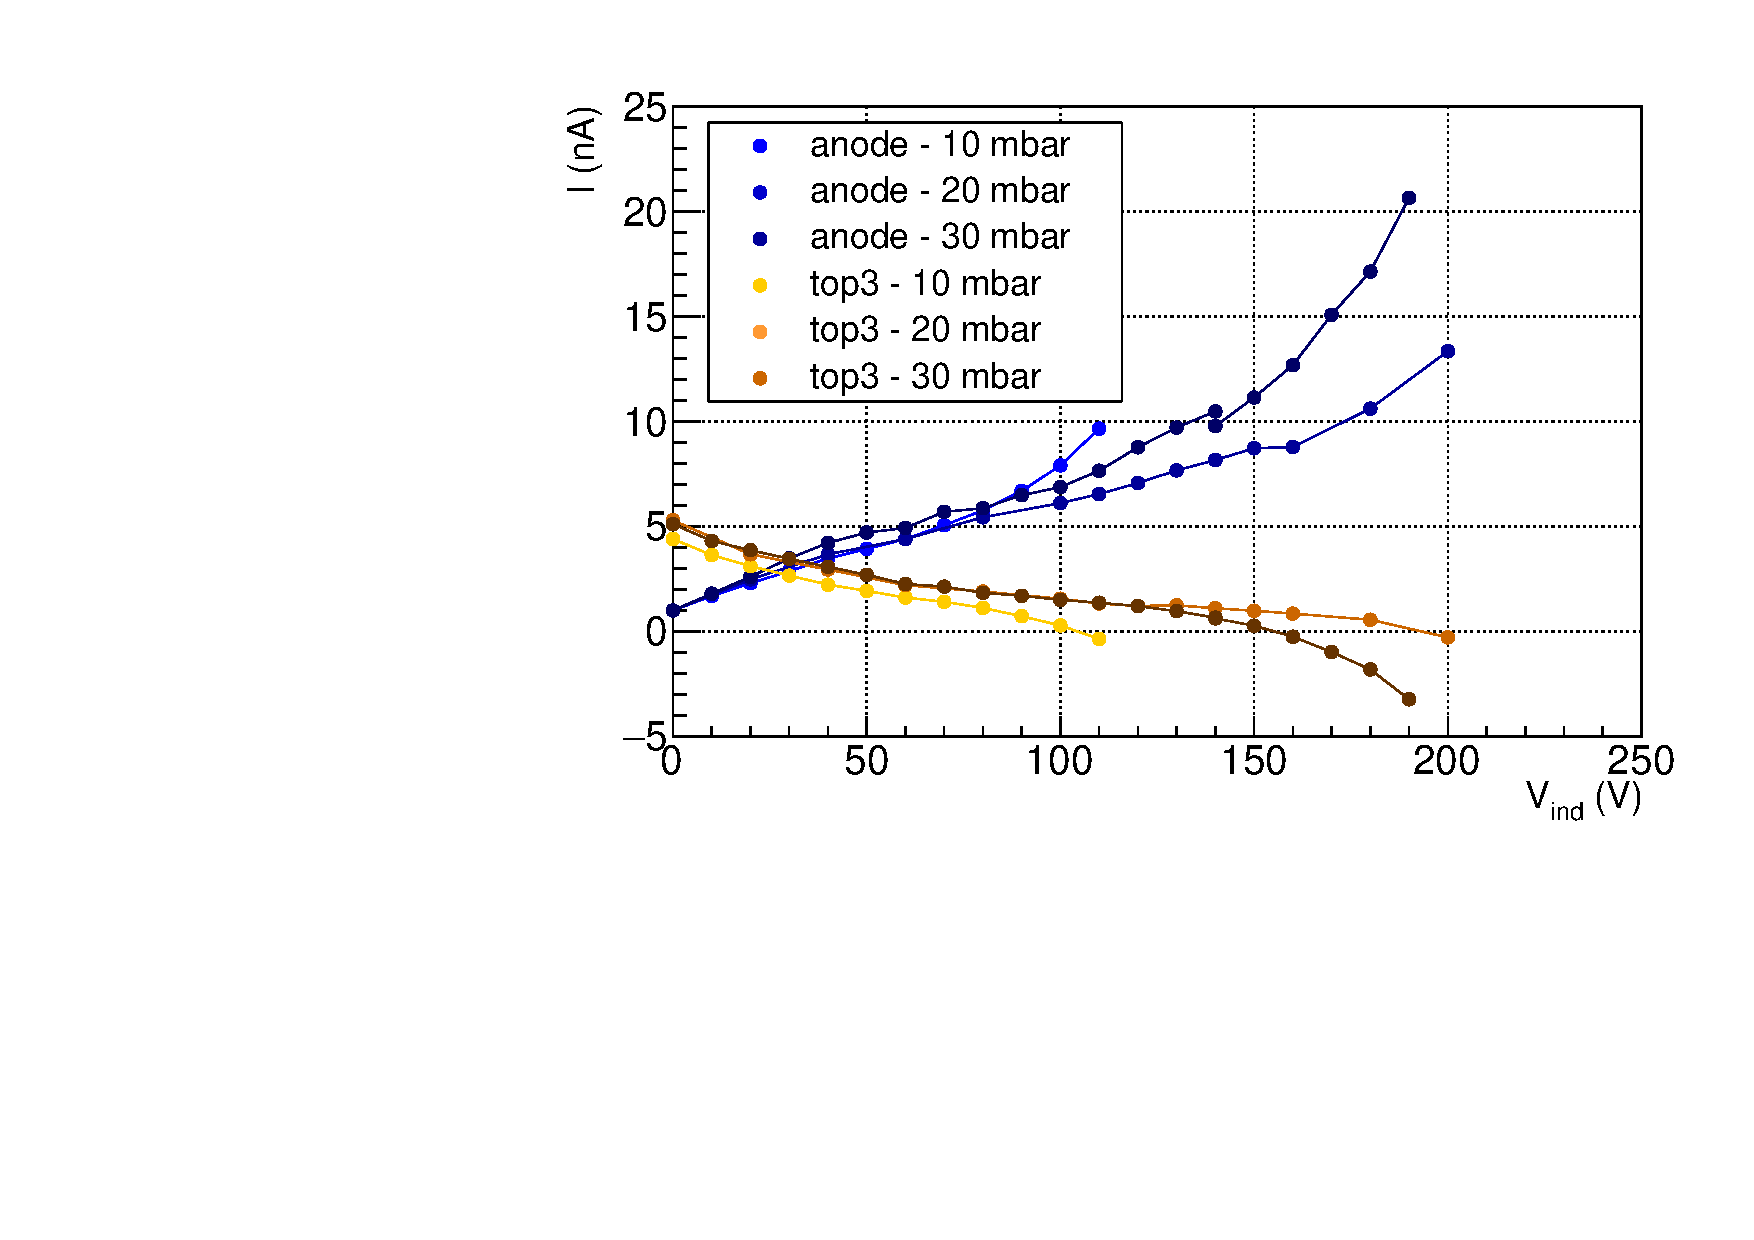
\includegraphics[width=0.97\textwidth]{Immagini/InductionScan_FULL_AnodeComp_2.pdf}
	\caption{Comparison of the anode and top3 currents at pressure of 10, 20, 30 mbar.}
	\label{fig:induction_pressure_comps}
\end{figure}

\clearpage

\subsubsection{Scan on \Vthgem}
In this section the scan of \Vthgem{} are shown. The the \Vind{} and \Vdrift{} values were kept 
fix while the \Vthgem{} was ranging from 0 to a maximum value, corresponding to the discharge,at 
step of 5/10 V. 
Table~\ref{tab:FULLTHGEM_vthgem} shows a scheme of the configurations explored in the scans.
\begin{table} [!h]
	\begin{center}
		\renewcommand{\arraystretch}{1.2}
		\begin{tabular} {ccccccccc}
			P (mbar) & & \Vind{} (V) & & \Vdrift{} (V) & & \Vthgem{} (V) & & run\\
			\toprule[0.1em]
			%\hline
			30	& &	120	& &	1000	& & 180$\div$235 & & 29-39 \\
			20	& &	100	& & 1000	& & 150$\div$215 & & 112-123 \\
			11	& & 70	& & 600		& & 130$\div$210 & & 169-183 \\		
			9.3 & & 50  & & 400     & &              & & 440-444 \\   
			\bottomrule[0.1em]
		\end{tabular}
	\end{center}
	\caption{P, \Vind{}, \Vdrift{} and the explored \Vthgem{} range used in the \Vthgem{} scans.} 
	\label{tab:FULLTHGEM_vthgem}
\end{table}
Figure~\ref{fig:thgem_FULLTHGEM_30mbar}, \ref{fig:thgem_FULLTHGEM_20mbar} and 
\ref{fig:thgem_FULLTHGEM_10mbar} show the currents vs \Vthgem{} plot for pressure of 30 20 and 10 
mbar respectively. A typical exponential trend for increasing \Vthgem is evident in all the 
plot\footnote{The exponential bheaviour for the anode is confirmed looking at the Multiplication 
Factor plot in the following.}.
\begin{figure}[!t]
	\centering
	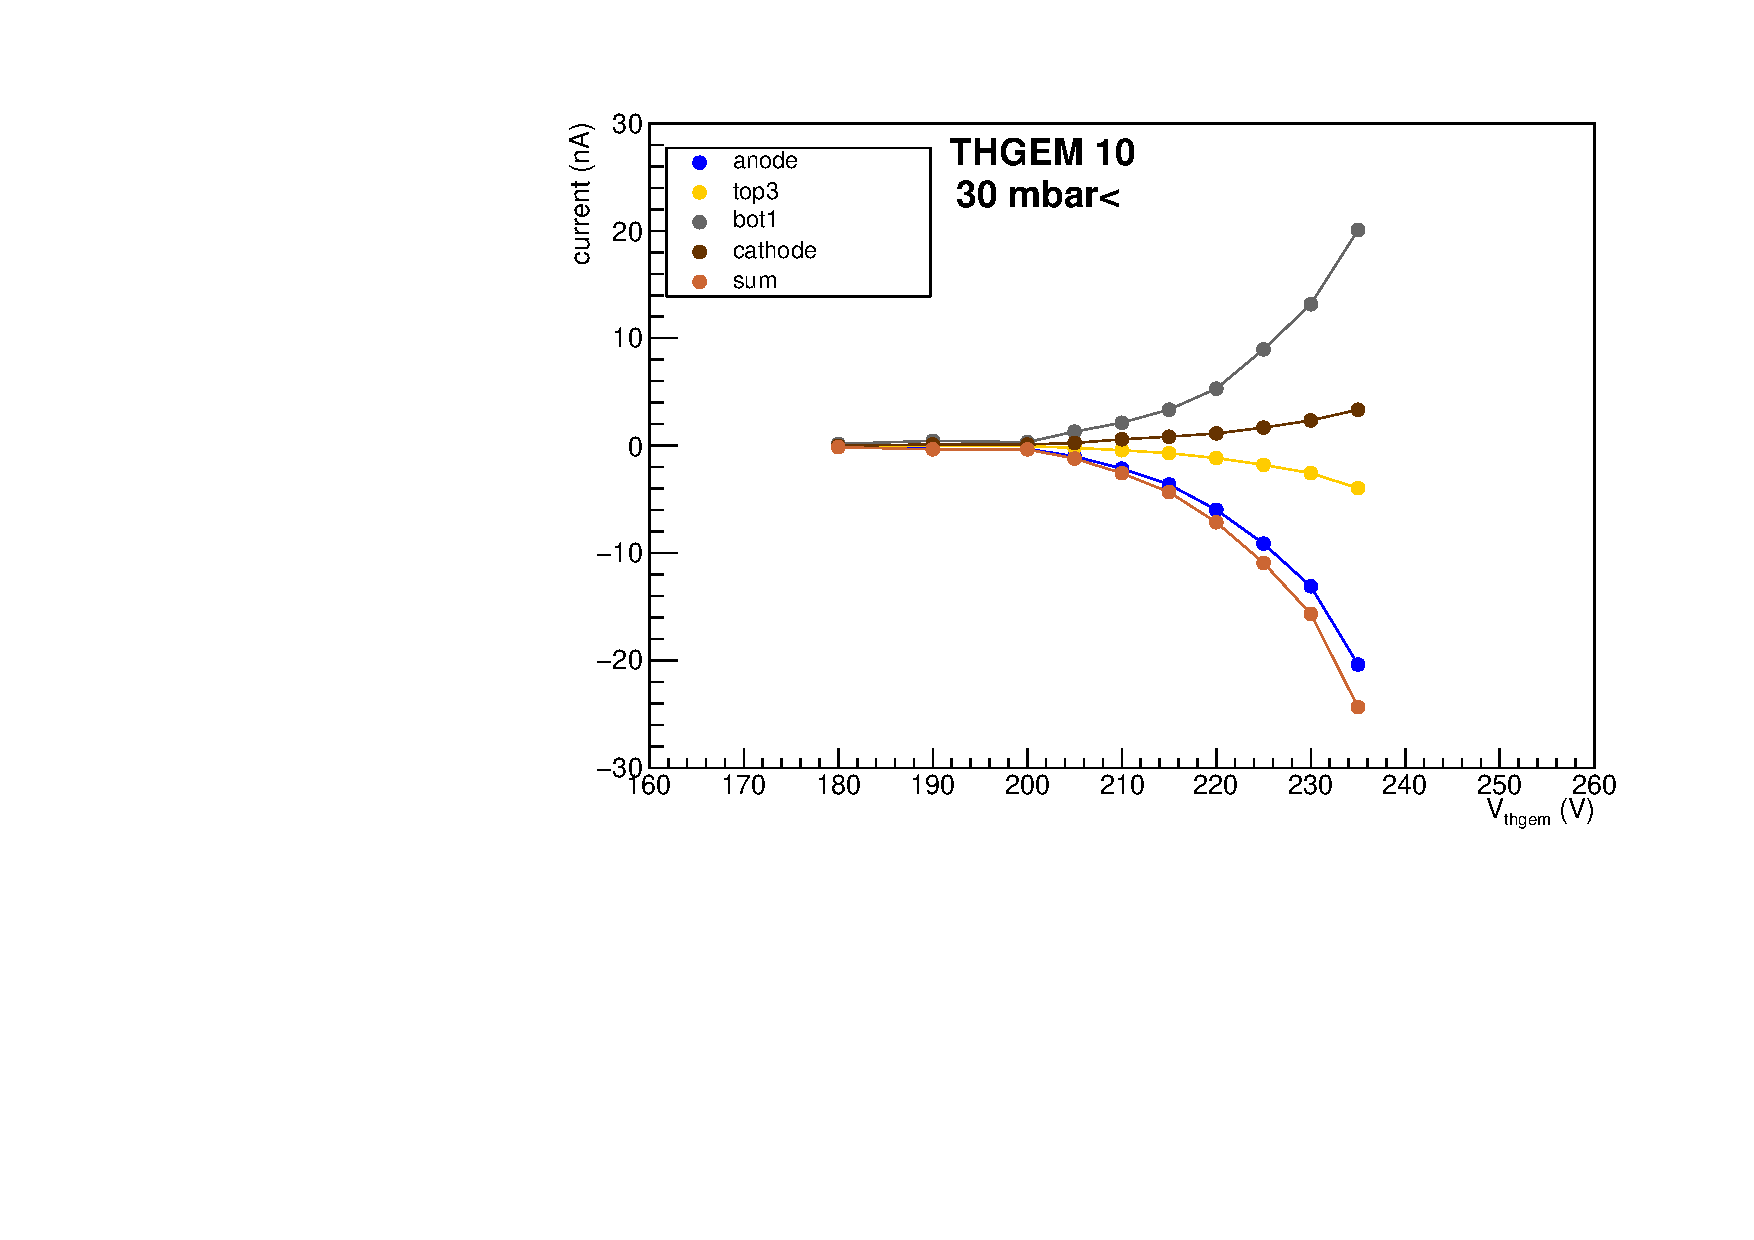
\includegraphics[width=\textwidth]{Immagini/thgemScan_THGEM10_30mbar.pdf}
	\caption{Currents measured during the scan on the voltage \Vthgem{} across each FULL THGEM 
	at 30~mbar.}
	\label{fig:thgem_FULLTHGEM_30mbar}
\end{figure}

\begin{figure}[!htb]
	\centering
	\subfigure[]{ 
	  \label{fig:thgem_FULLTHGEM_20mbar} 
	  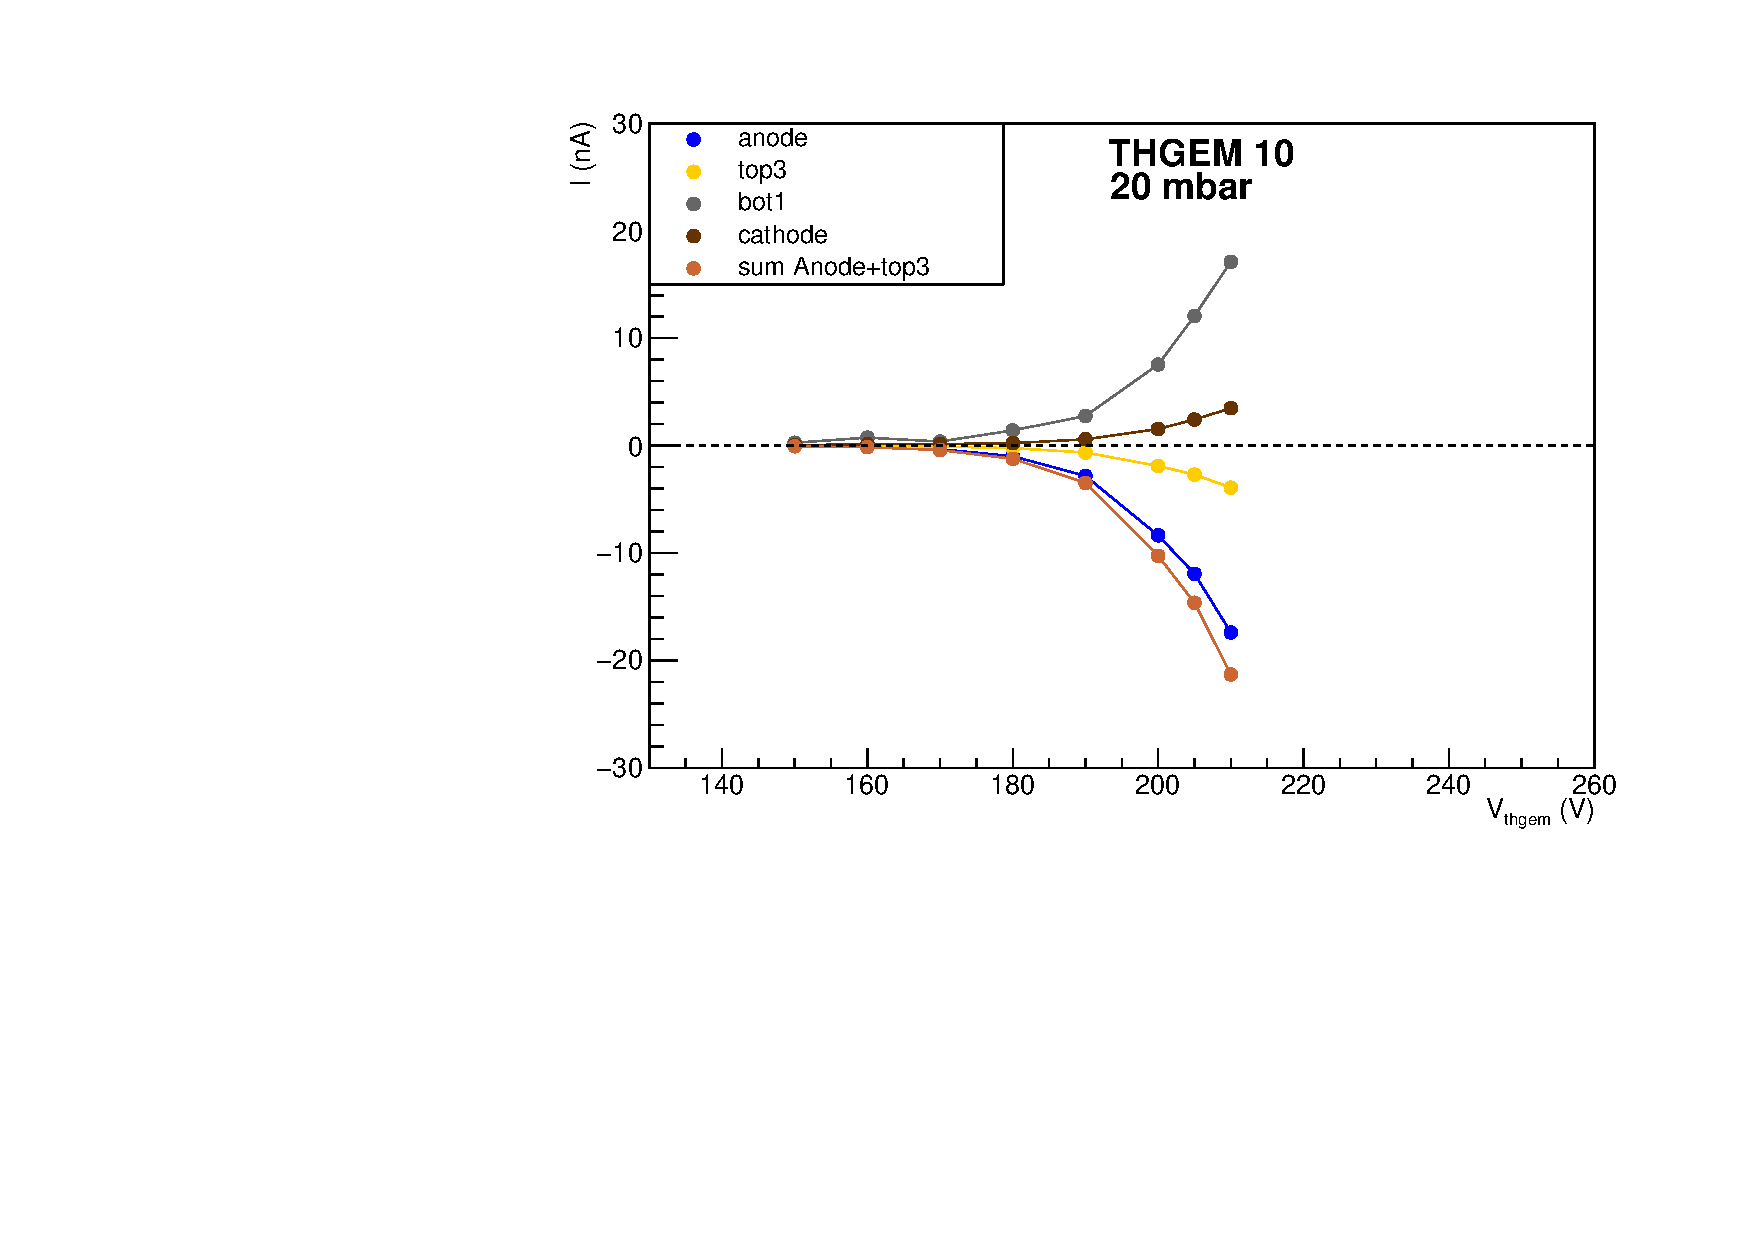
\includegraphics[width=0.96\textwidth]{Immagini/thgemScan_THGEM10_20mbar.pdf}}
	\subfigure[]{ 	
	  \label{fig:thgem_FULLTHGEM_10mbar} 
	  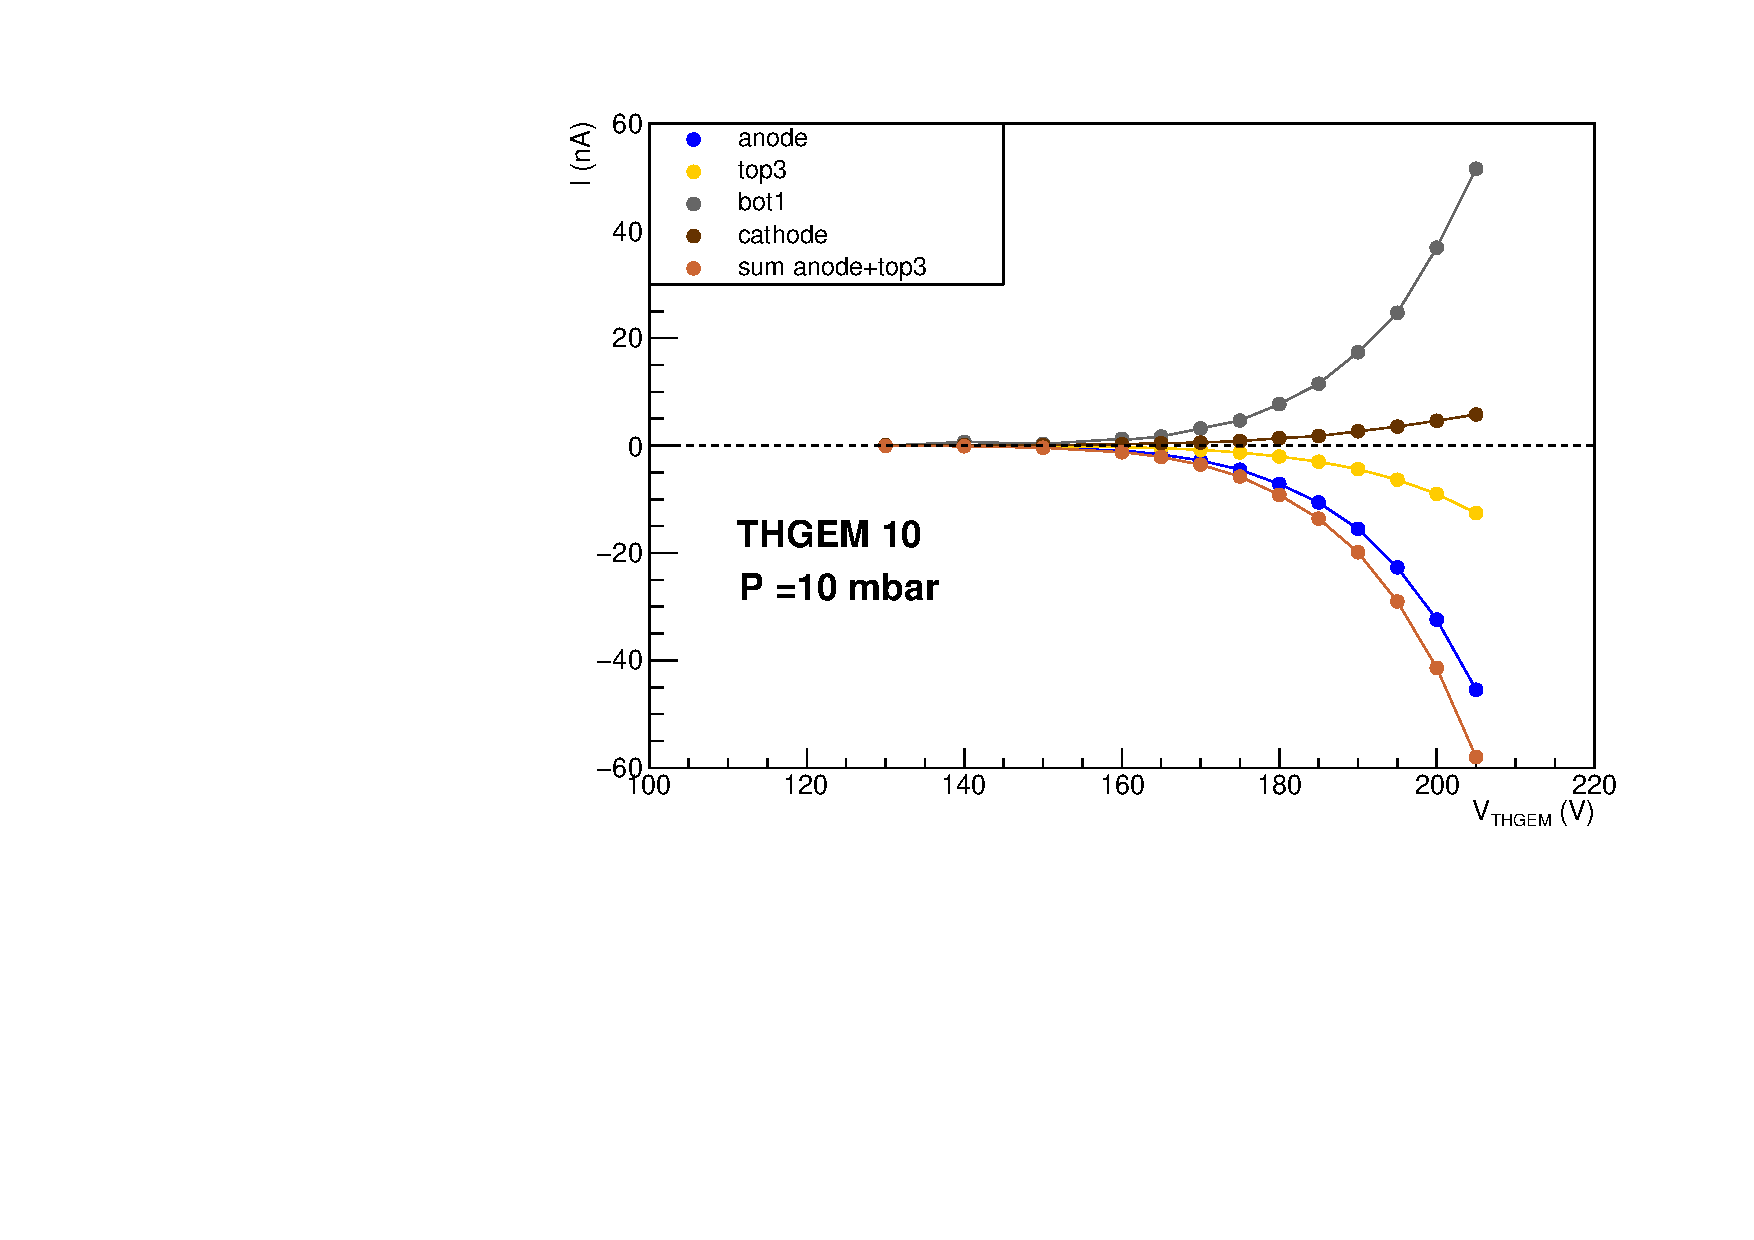
\includegraphics[width=0.96\textwidth]{Immagini/thgemScan_THGEM10_10mbar.pdf}}
        \caption{Currents measured during the scan on the voltage \Vthgem{} across each FULL THGEM: 
        in (a) with P~=~20~mbar, \Vind~=~100~V and \Vdrift~=~1000~V, in (b) with P~=~11~mbar, 
        \Vind~=~70~V and \Vdrift~=~600~V.}
	\label{fig:thgem_FULLTHGEM_20and10mbar}
\end{figure}

From these measurements, the multiplication factors (MFs) were evaluated as a function of \Vthgem{} 
for different pressures.
The MF have been calculated in the following way. Knowing the energy of the incident particles 
($\alpha$ at 5.485 MeV) the pressure of the gas and the length of the track it is possible
to calculate the energy lost by $\alpha$ in the gas. From this, knowing the mean energy for
ion-electron pair creation, it is possible to calculate the number of primary electron produced
per particle. Knowing the number of $\alpha$-particle enetering the detector per second
is possible to have an estimate of the total number of primary electron produced per second.
From this value and the anodic current is straightforward to get the MF.

The MFs are show	n in Figure~\ref{fig:multiplication_factor_FULL}, the curves seems to follow
an exponential law in good approximation.
For a fixed value of \Vthgem, the MF decreases with increasing the pressure as expected.
\begin{figure}[!t]
	\centering
	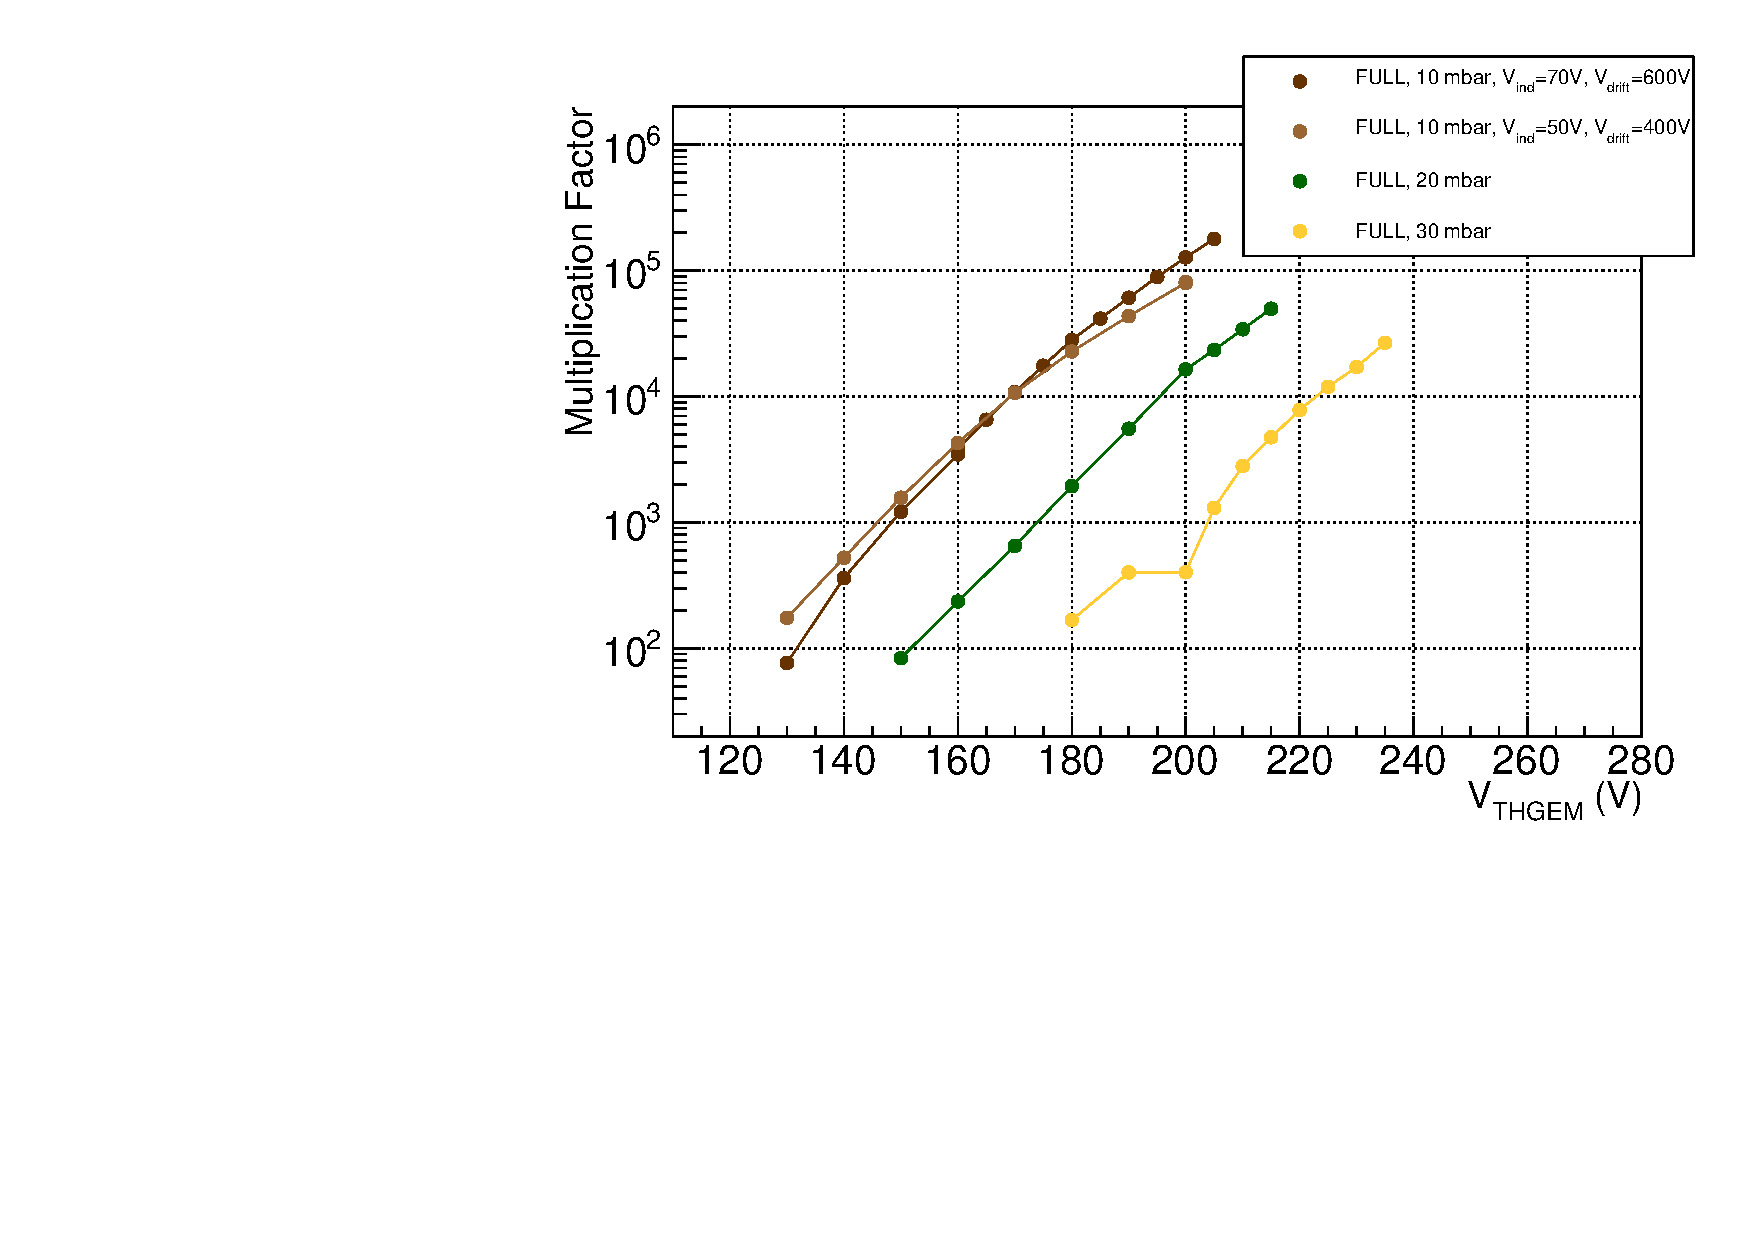
\includegraphics[width=\textwidth]{Immagini/MF_FULL_THGEM_noBeam.pdf}
	\caption{The multiplication factors evaluated for the FULL THGEM as a function of \Vthgem{} 
	and pressure.}
	\label{fig:multiplication_factor_FULL}
\end{figure}
The maximum values of the \Vthgem reachable depends obviously on the gas pressure but 
seems not to follow a simple decreasing law.

\clearpage

\subsubsection{Scan on \Vdrift}
In this section the behaviour of the prototype as a function of \Vdrift{} have been studied.
As in previous case, while pressure, \Vind{} and \Vthgem{} were kept fixed, \Vdrift{} was varied 
from 0~V (or 100~V) to the discharge voltage\footnote{Discharge is most probably due to the 
"effetto punta" between conductor elements at the same potential of the cathode with the ground.}, 
which depends on the gas pressure; in fact for P~=~30~mbar it was 1600~V, for P~=~20~mbar it was 
1200~V, and for P~=~11~mbar it was 800~V.
The \Vdrift step was 50~V for P~=~11~mbar, and 100~V for the other cases.
In Table~\ref{tab:FULLTHGEM_vdrift} a scheme of the configuration of the  prototype is shown.
\begin{table} [!h]
	\begin{center}
		\renewcommand{\arraystretch}{1.2}
		\begin{tabular} {ccccccc}
			P (mbar) & & \Vind{} (V) & & \Vthgem{} (V) & & run\\
			\toprule[0.1em]
			%\hline
			30	& &	120	& &	220 & & 40-60\\
			20	& &	100	& & 205 & & 124-138\\
			11	& & 70	& & 190 & & 184-200\\
			11	& & 70	& & 170 & & 201-206\\
			9.3 & & 50  & & 160 & & 440-444\\
			\bottomrule[0.1em]
		\end{tabular}
	\end{center}
	\caption{The values of pressure (P), \Vind{} and \Vthgem{} adopted for the study on \Vdrift.} 
	\label{tab:FULLTHGEM_vdrift}
\end{table}

The result of the scan at 30~mbar is shown in Figure~\ref{fig:drift_FULLTHGEM_30mbar}. 

The anodic current seems not be dependent on the values of the \Vdrift. In fact the value of the 
anodic current is basically constant but for the point at \Vdrift=0V where, surprisingly, a 
value  of the anodic current different from zero is observed. For the sake of curiosity further 
measurements were done to investigate the behaviour of the prototype at very low \Vdrift~=~30~V, 
20~V, 20~V, and 5~V. Till so small values\footnote{for \Vdrift=5V the elctric field in the drift region
is about $5/20\; \mbox{(V/cm)}= 250 \; \mbox{(mV/cm)}$.} the anodic current is still constant and do not 
decreases, for a magnified view see Figure~\textcolor{red}.

Conclusion are that the \Vdrift at so small rate of event do not affects the collection of the
prmary electron even at very small \Vdrift. Concerning the fact that at \Vdrift=0V we still
see the anodic current we suspect that the PICO picoammeter or the CAEN power supply
introduce some very small \Vdrift that is enough to collect a large fraction of the primary
electron\footnote{Some simulation could be very usefull to understand such phenomena.}.
\begin{figure}[htbp]
	\centering
	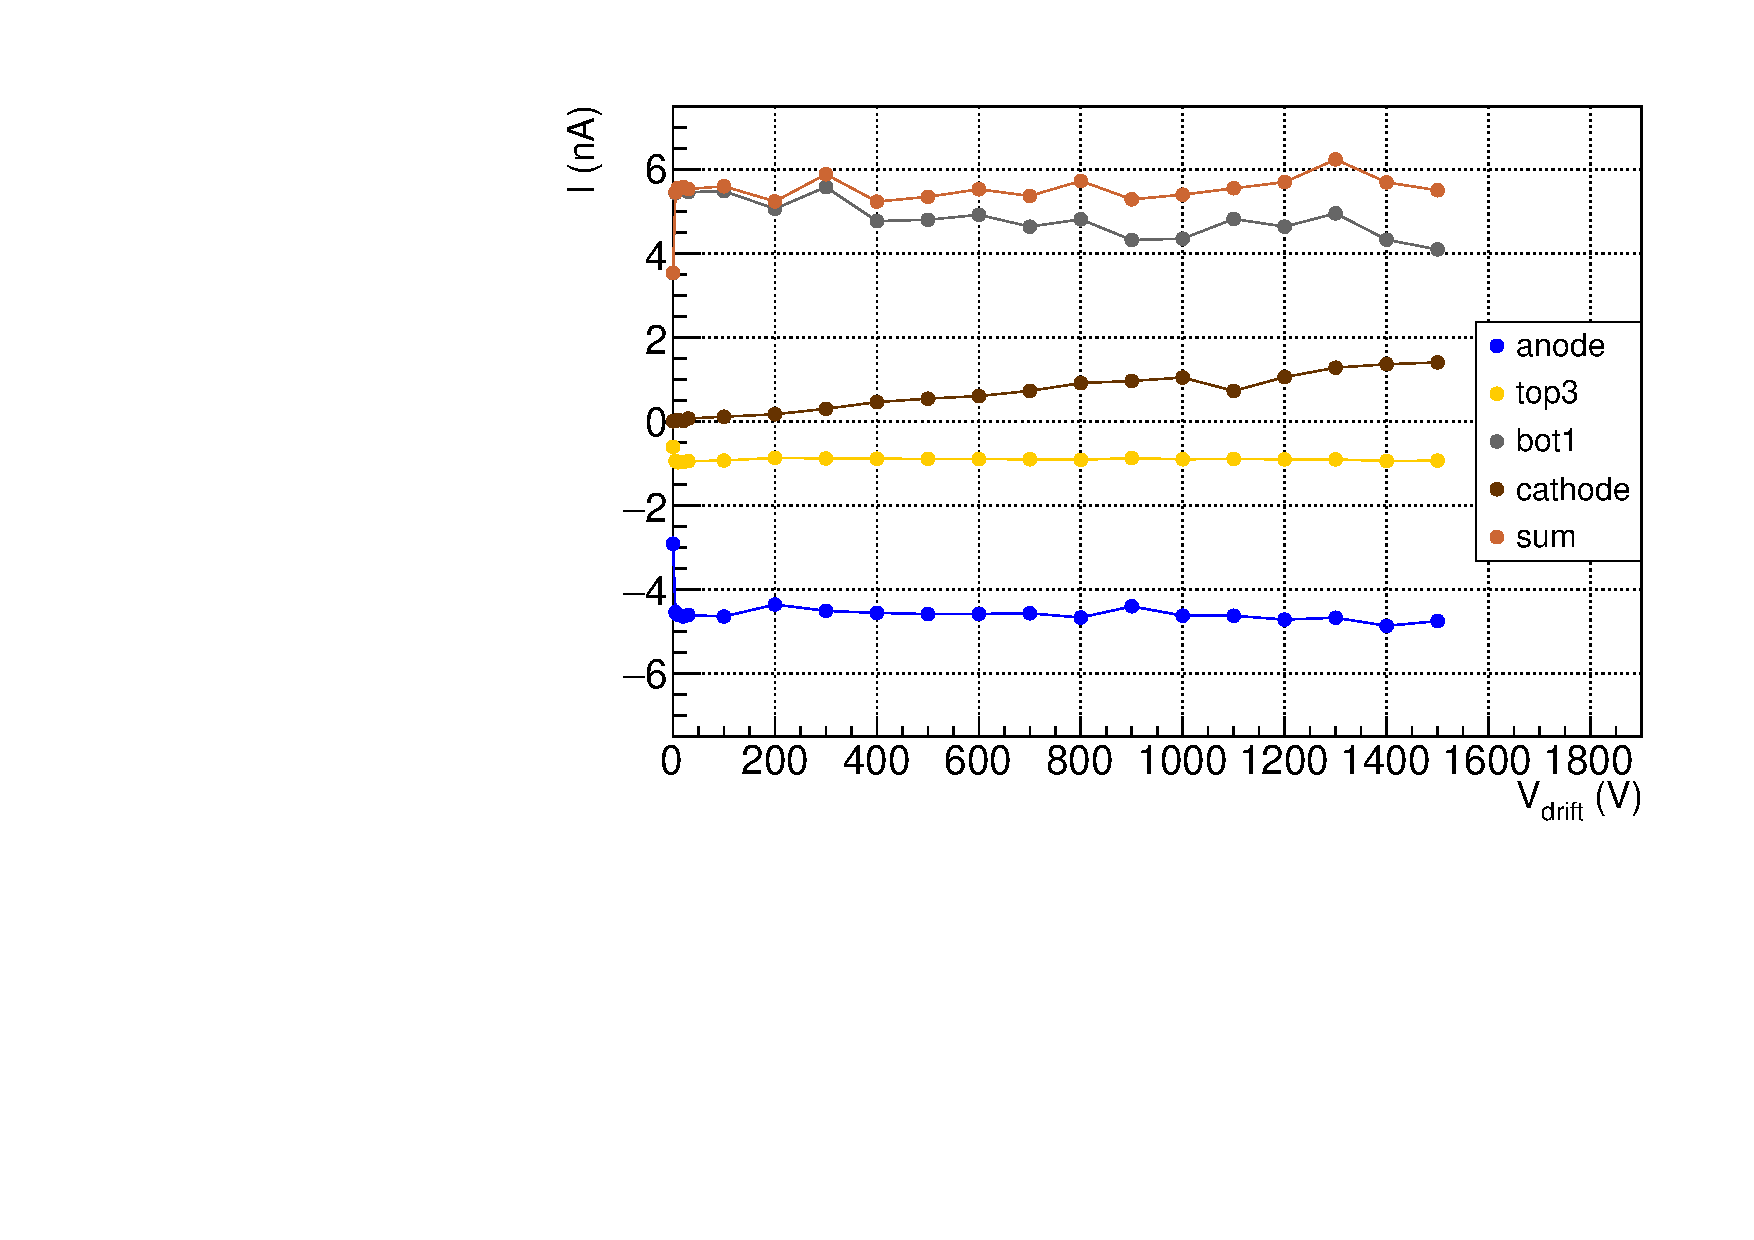
\includegraphics[width=\textwidth]{Immagini/driftScan_FULL_30mbar_r40-60.pdf}
	\caption{Currents measured during the scan on the voltage \Vdrift{} across the drift region at 30~mbar.}
	\label{fig:drift_FULLTHGEM_30mbar}
\end{figure}
\begin{figure}[htbp]
	\centering
	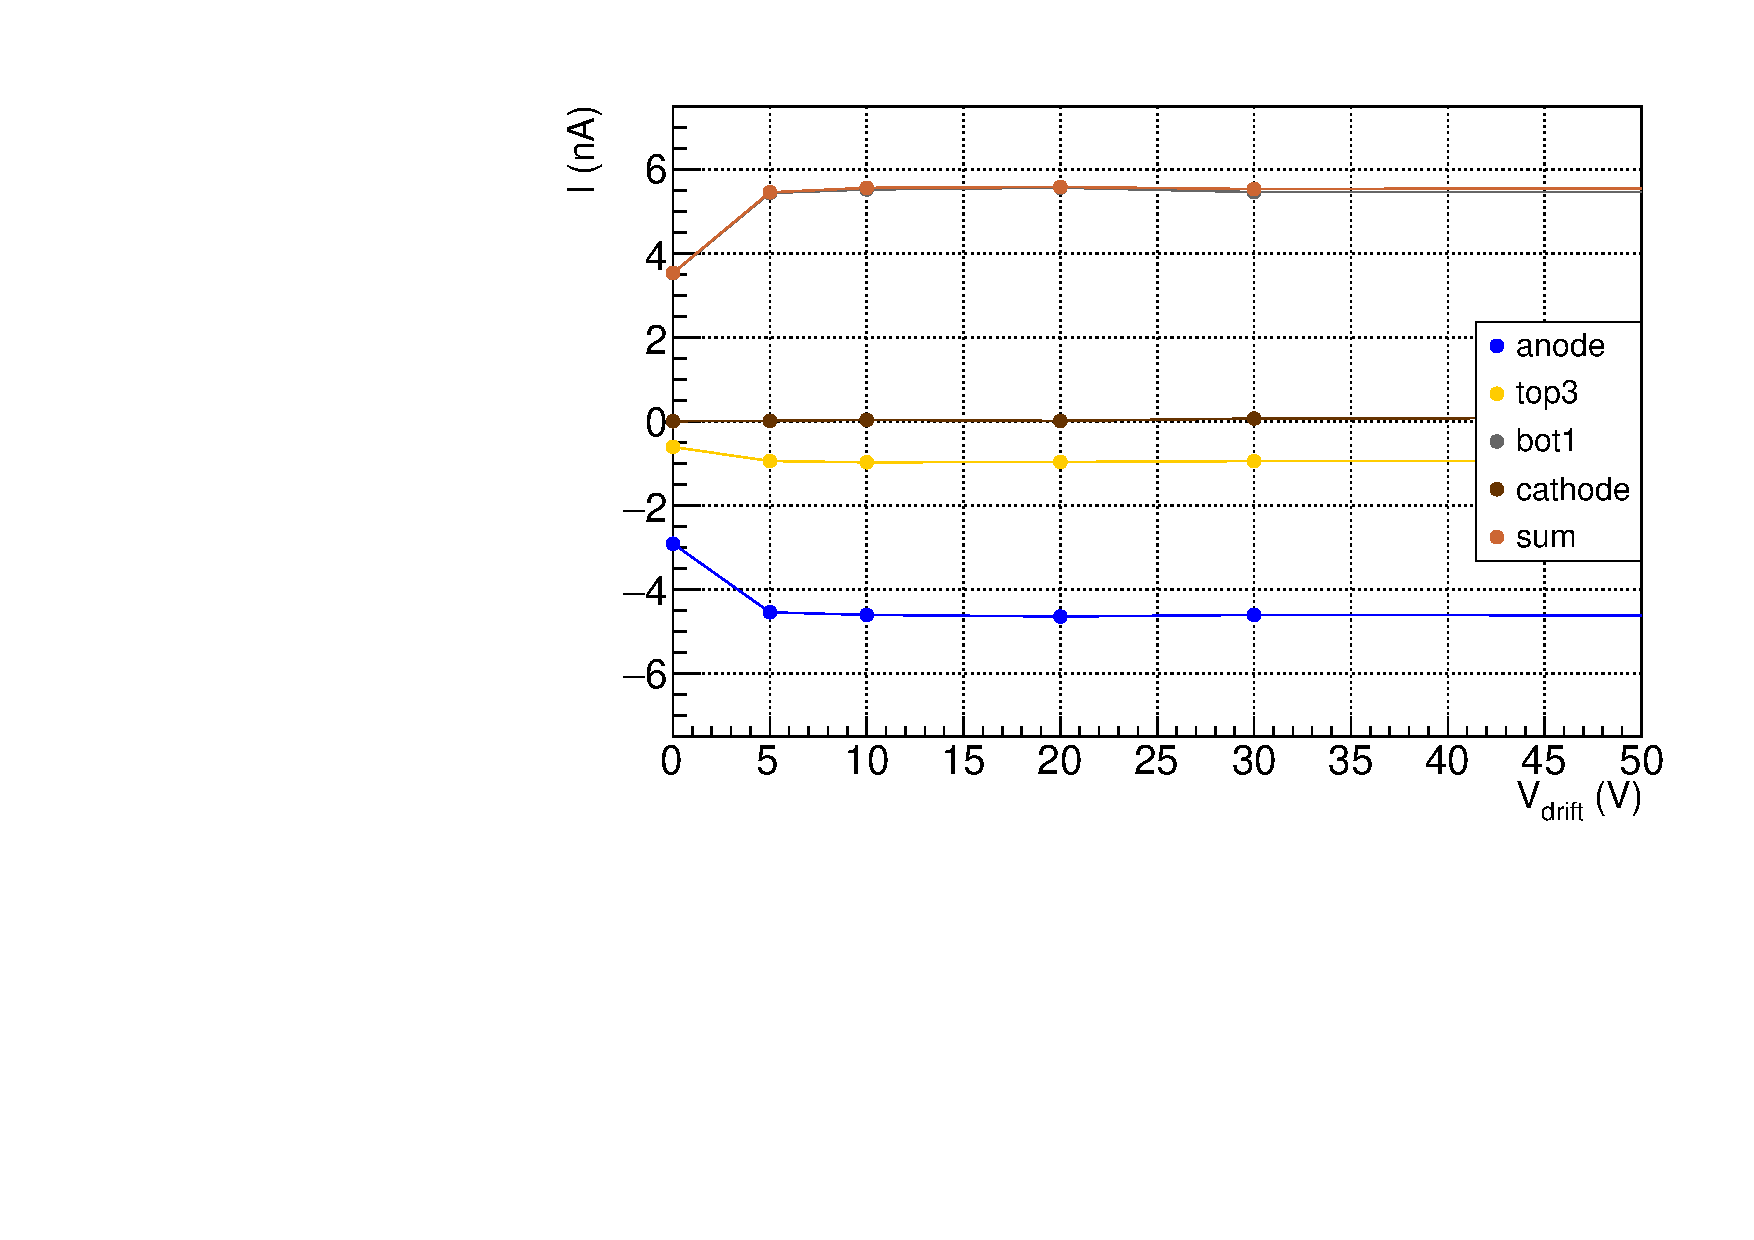
\includegraphics[width=\textwidth]{Immagini/driftScan_FULL_30mbar_r40-60_zoom1.pdf}
	\caption{Magnification of Fig. \ref{fig:drift_FULLTHGEM_30mbar}.}
	\label{fig:drift_FULLTHGEM_30mbar_mag}
\end{figure}

In Figure~\ref{fig:drift_FULLTHGEM_30mbar} the orange line represents, in this case, the sum of the
cathode and bot1 currents. This quantity is important to estimate the Ion Backflow (IB). 

The scans at 20 and 11~mbar are shown, respectively, in Figure~\ref{fig:drift_FULLTHGEM_20mbar} and~\ref{fig:drift_FULLTHGEM_11mbar}.
\begin{figure}[!htb]
	\centering
	\subfigure[]{ \label{fig:drift_FULLTHGEM_20mbar} 
	  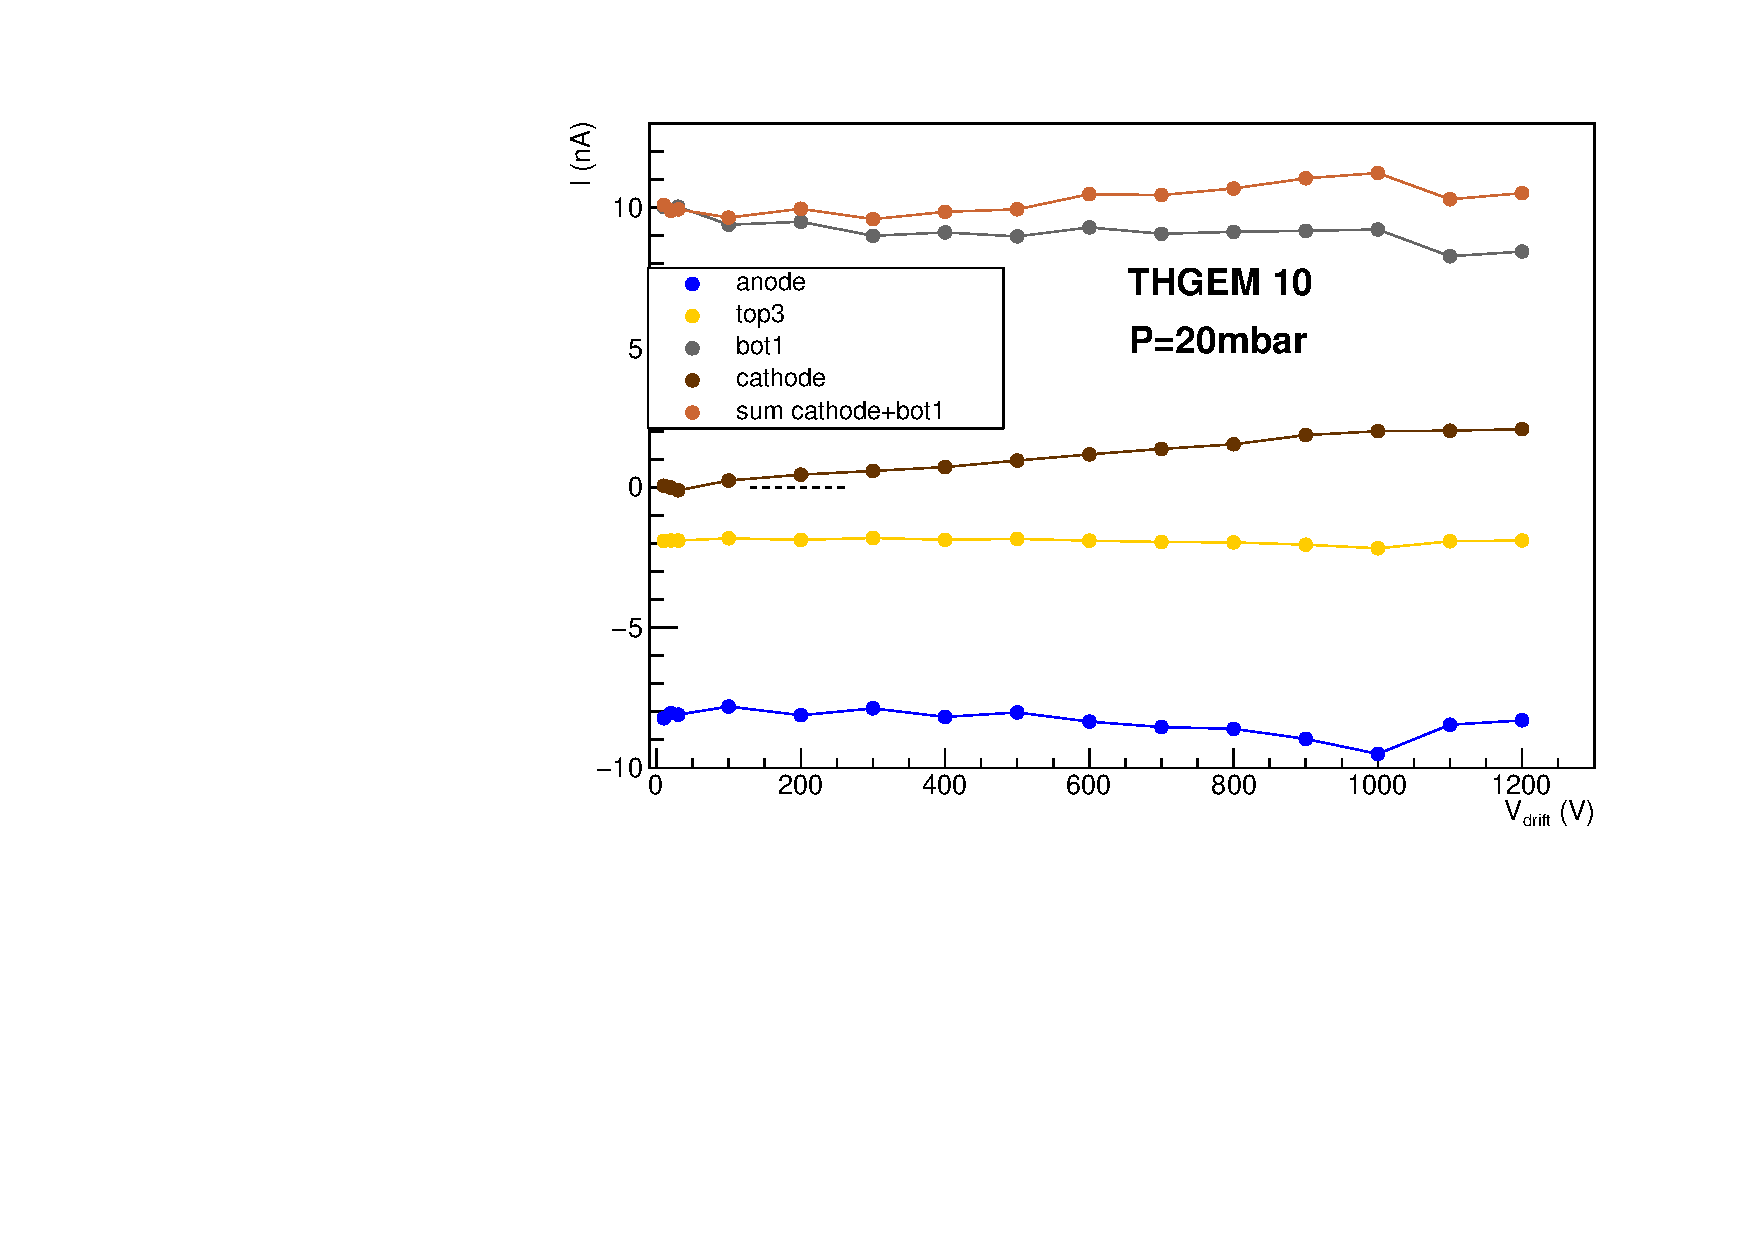
\includegraphics[width=0.96\textwidth]{Immagini/driftScan_THGEM10_20mbar.pdf}}
	\subfigure[]{ 	\label{fig:drift_FULLTHGEM_11mbar}
	  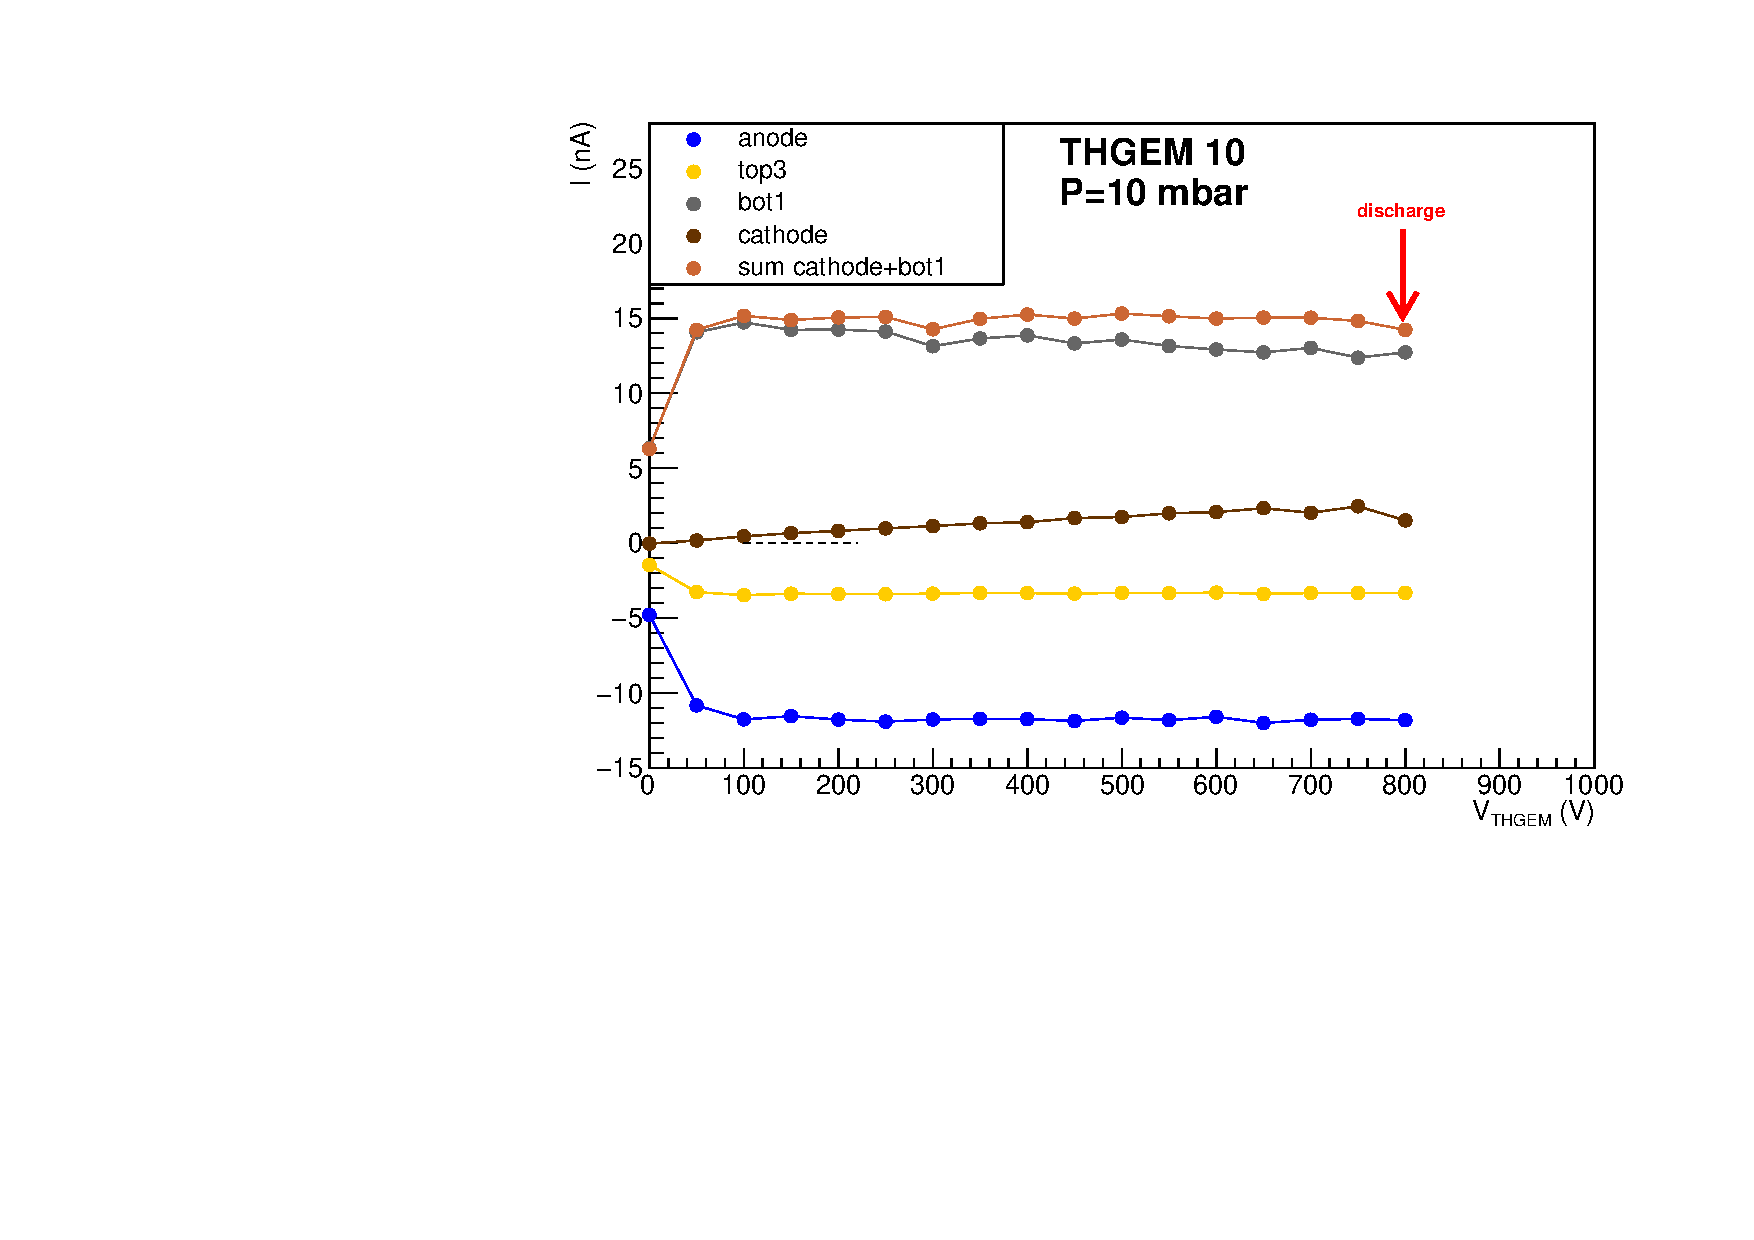
\includegraphics[width=0.96\textwidth]{Immagini/driftScan_THGEM10_10mbar.pdf}}
	\caption{Currents measured during the scan on the voltage \Vdrift{} across the drift region: in 
	(a) at 20~mbar, in (b) at 11~mbar.}
	\label{fig:drift_FULLTHGEM_other_pressure}
\end{figure}
%\textcolor{red}{Aggiungere plot sul backflow}
The IB, defined of the ration between the current flowing in the cathode and the TNC that is the sum
of current flowing in the anode and in the top3, have been also plotted as a function of the \Vdrift.

In Figure~\ref{fig:ion_backflow_FULL} is evident the trend of the ion backflow that increases, almost
linearly for increasing \Vdrift{}. Its value seems not be depending on the pressure.
In Figure~\ref{fig:ion_backflow_FULL_F} The IBF for three different ressure is shown as a function of
the reduced electric field E/p.

\begin{figure}[htbp]
	\centering
	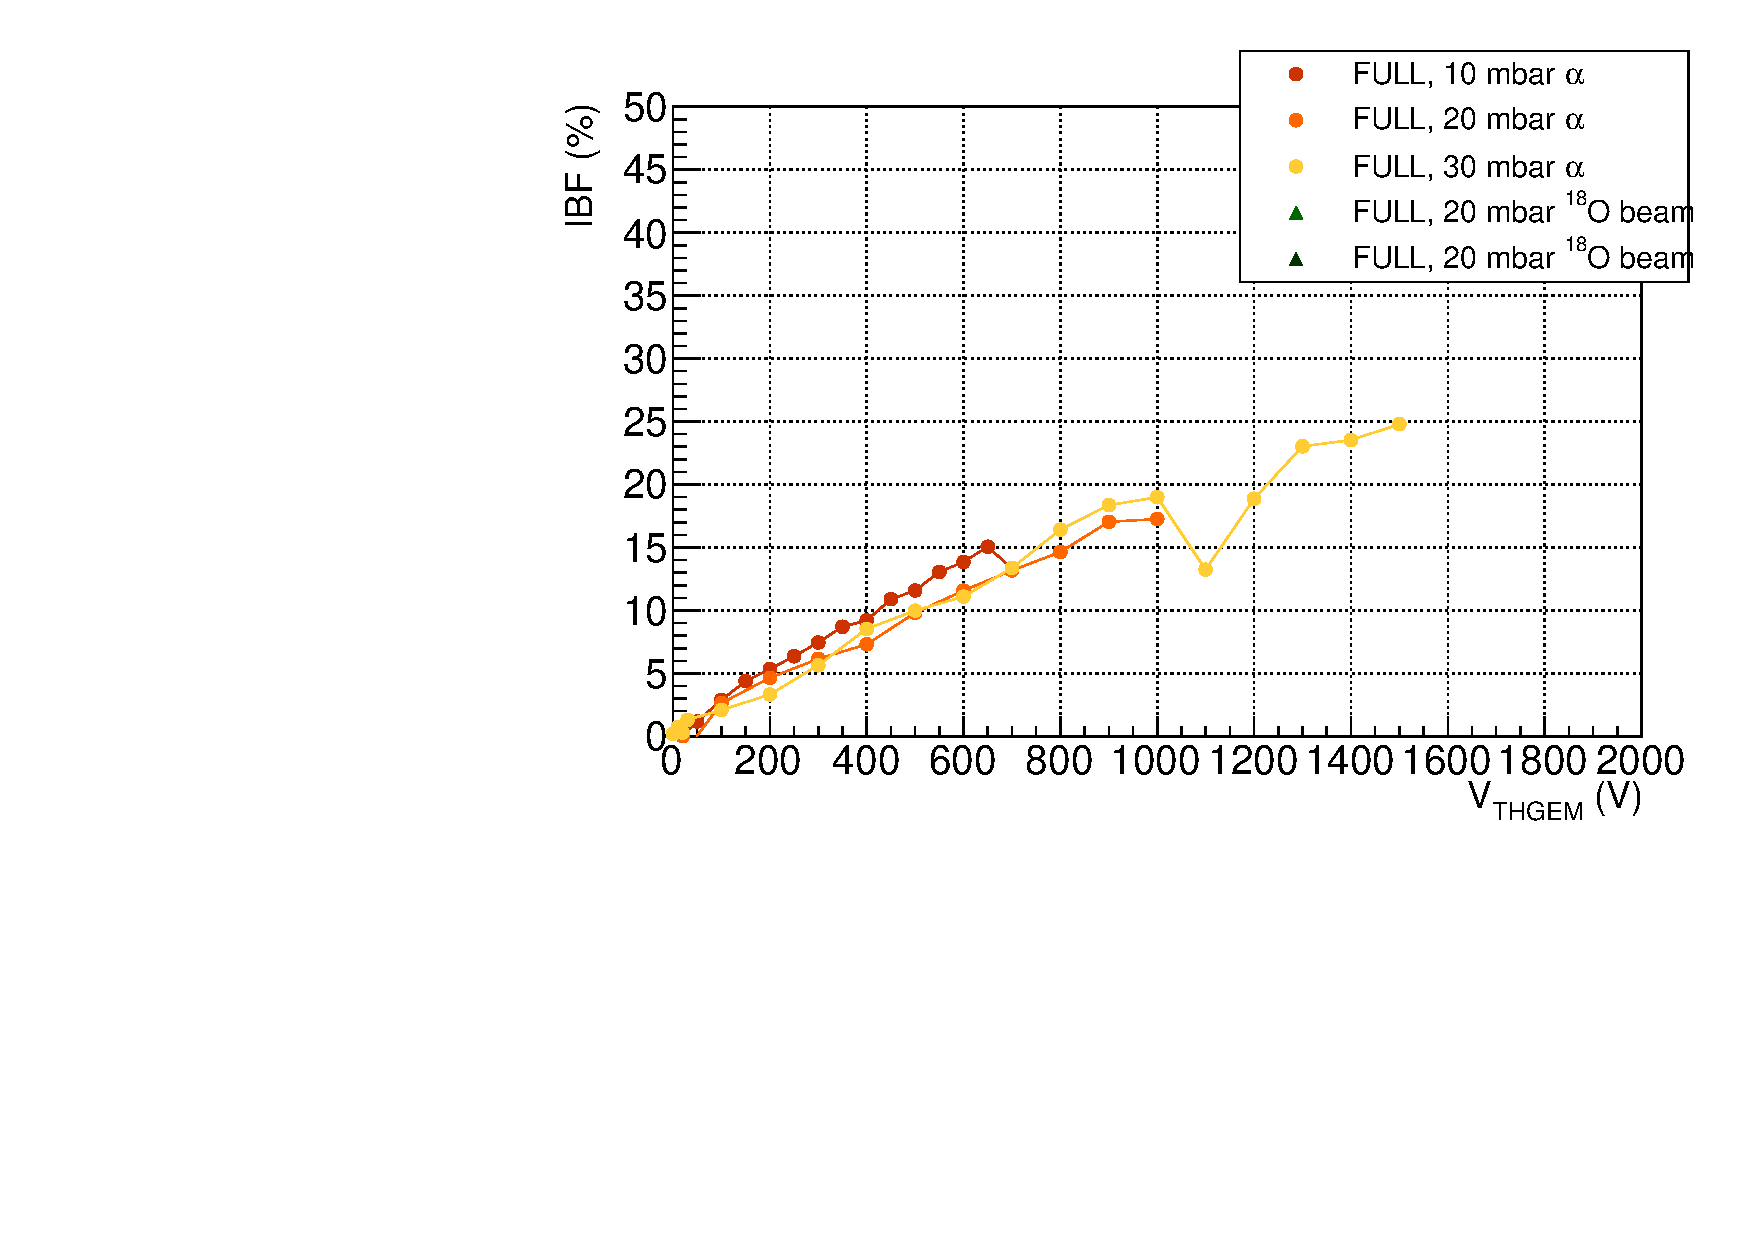
\includegraphics[width=\textwidth]{Immagini/IBF_FULL_Comparison_nobeam.pdf}
	\caption{The ion backflow as a function of \Vdrift{} for the three examined pressures.}
	\label{fig:ion_backflow_FULL}
\end{figure}
\begin{figure}[htbp]
	\centering
	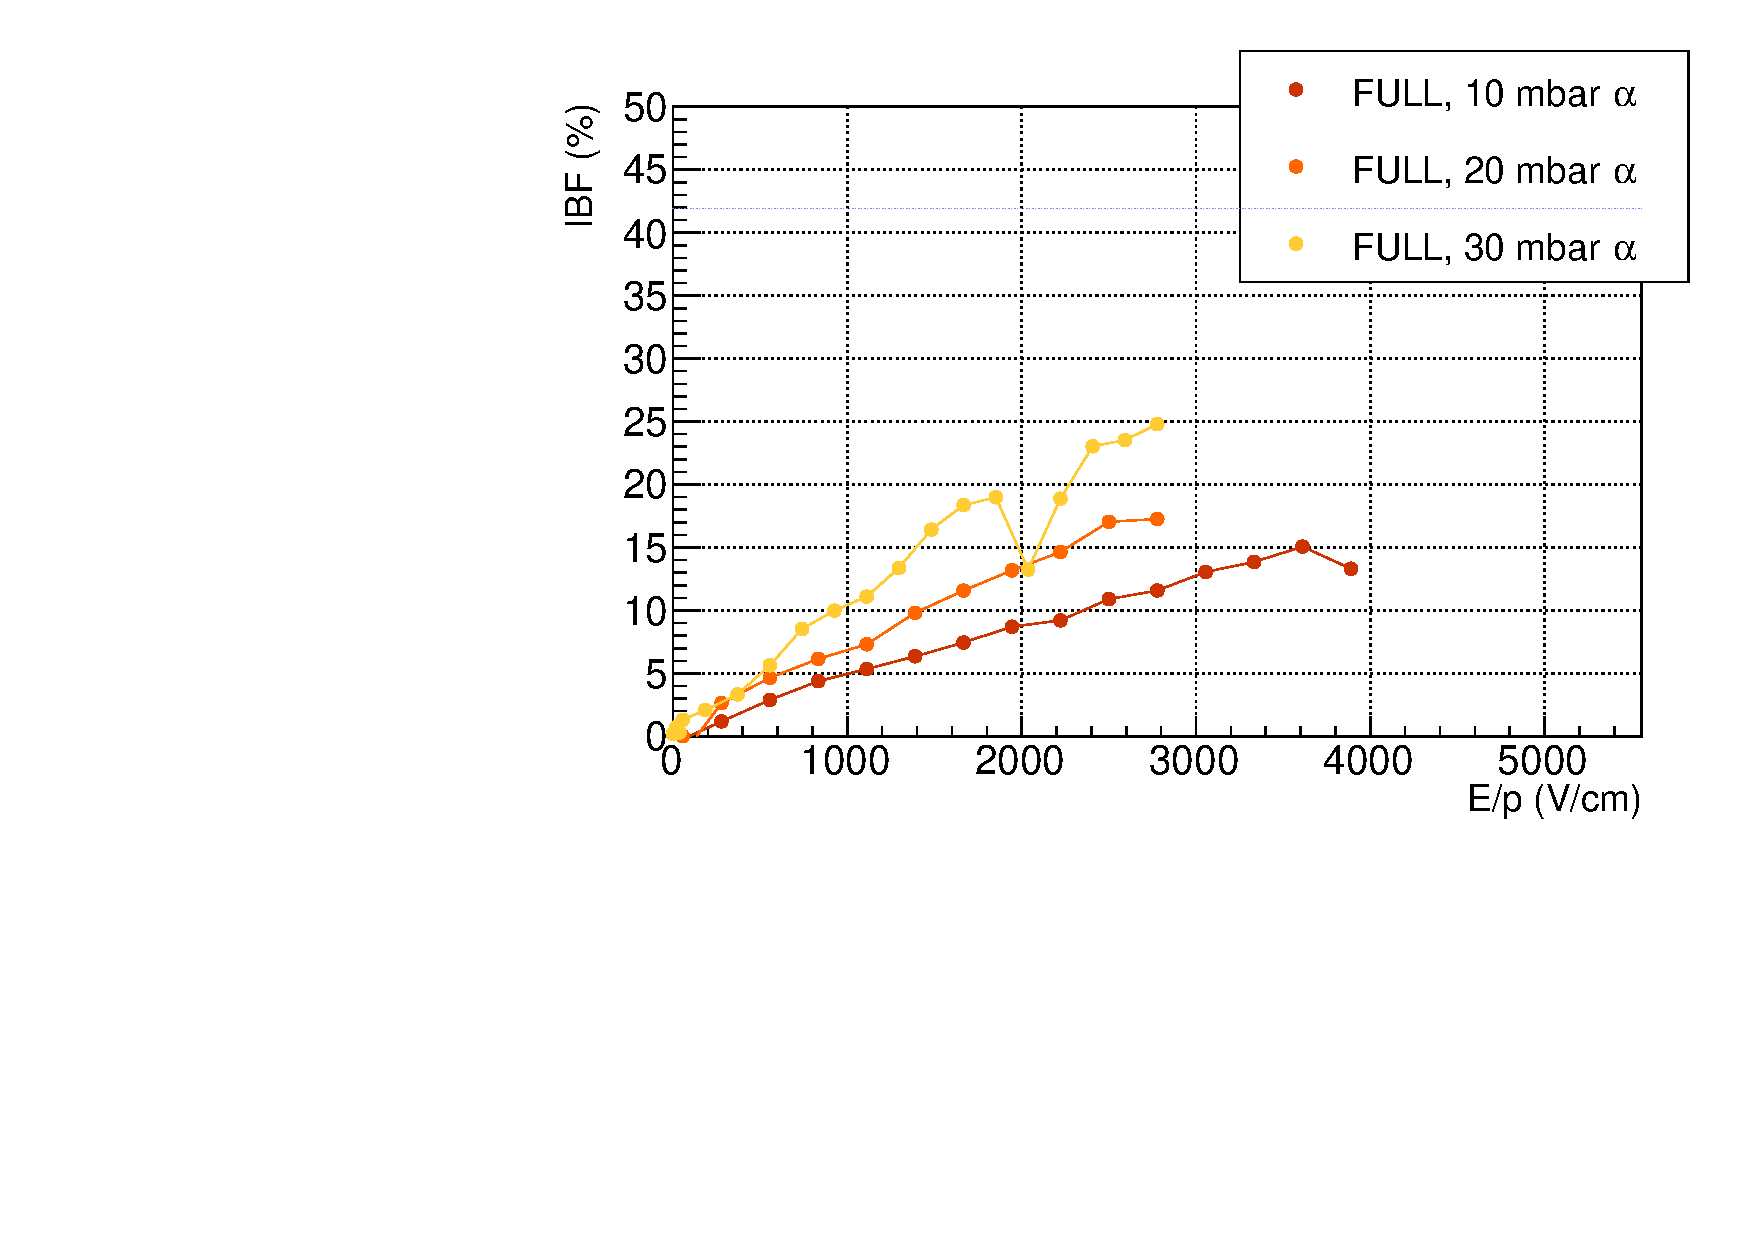
\includegraphics[width=\textwidth]{Immagini/IBF_FULL_Comparison_nobeam_F.pdf}
	\caption{As Fig. \ref{fig:ion_backflow_FULL} but as a function of the reduced electric field
	instead of voltage.}
	\label{fig:ion_backflow_FULL_F}
\end{figure}
\clearpage

\subsection{ROW THGEM}
The same studies perfomed on the FULL THGEM have been repeated on the ROW THGEM. We shortly recall 
that the main difference respect to the FULL THGEM is the significantly lower number of holes.
Therefore we expect that, for similar condition, the currents on the ROW THGEM are smaller compared 
to those of the FULL THGEM. Moreover this make difficult to estimate the MF since we do not know 
the actual number of primary electrons that reach the multiplication stage (the holes). In fact, 
part of the electron reach the no-hole region and therefore are not multiplied while an unknown 
fraction of primary electron is funneled through the holes and therefore multiplied.

\subsubsection{Scan on \Vind}
The \Vind{} scan have been done fixing pressure,\Vthgem{} and \Vdrift{}\ and changing the \Vind{} 
at step 10/20~V from 0~V to the discharge value  that was 110 V fot  P~=~20,30~mbar and 180 V at 
P~=~40~mbar.
A summary scheme of the configurations used in the test is shown in Table~\ref{tab:ROWTHGEM_vind}.
\begin{table} [htbp]
	\begin{center}
		\renewcommand{\arraystretch}{1.2}
		\begin{tabular} {ccccccc}
			P (mbar) & & \Vthgem{} (V) & & \Vdrift{} (V) & & run\\
			\toprule[0.1em]
			%\hline
			20.6	& &	220	& &	800 & & 207-218 \\
			20.1	& & 210	& & 800 & & 364-378\\
			30	& &	240	& &	800 & & 233-244\\
			42	& &	260	& &	700 & & 283-299\\		
			\bottomrule[0.1em]
		\end{tabular}
	\end{center}
	\caption{The values of pressure (P), \Vthgem{} and \Vdrift{} adopted for the study of \Vind
	on ROW THGEM.} 
	\label{tab:ROWTHGEM_vind}
\end{table}
The two scans at 20~mbar are shown in Figure~\ref{fig:induction_ROWTHGEM_20mbar} 
and~\ref{fig:induction_ROWTHGEM_20mbar_bis}. The ROW THGEM behaviour is similar to that of the Full 
THGEM: i.e. raising the value of \Vind{}, the anodic current (blue line) increases, while the top3 
current (yellow line) approaches to zero. One difference respect to the Full THGEM is that the 
orange curve (TNC) here is slowly growing, while for the full THGEM there was a region where it was constant (a plateau) and after a given value of \Vind{} started to grow. Anyway since the TNC is 
growing for increasing value of \Vind, the expansion of the multiplication region out of the THGEM 
holes is most probably occurring also for the ROW THGEM.
\begin{figure}[!htb]
	\centering
	\subfigure[]{ \label{fig:induction_ROWTHGEM_20mbar} 
	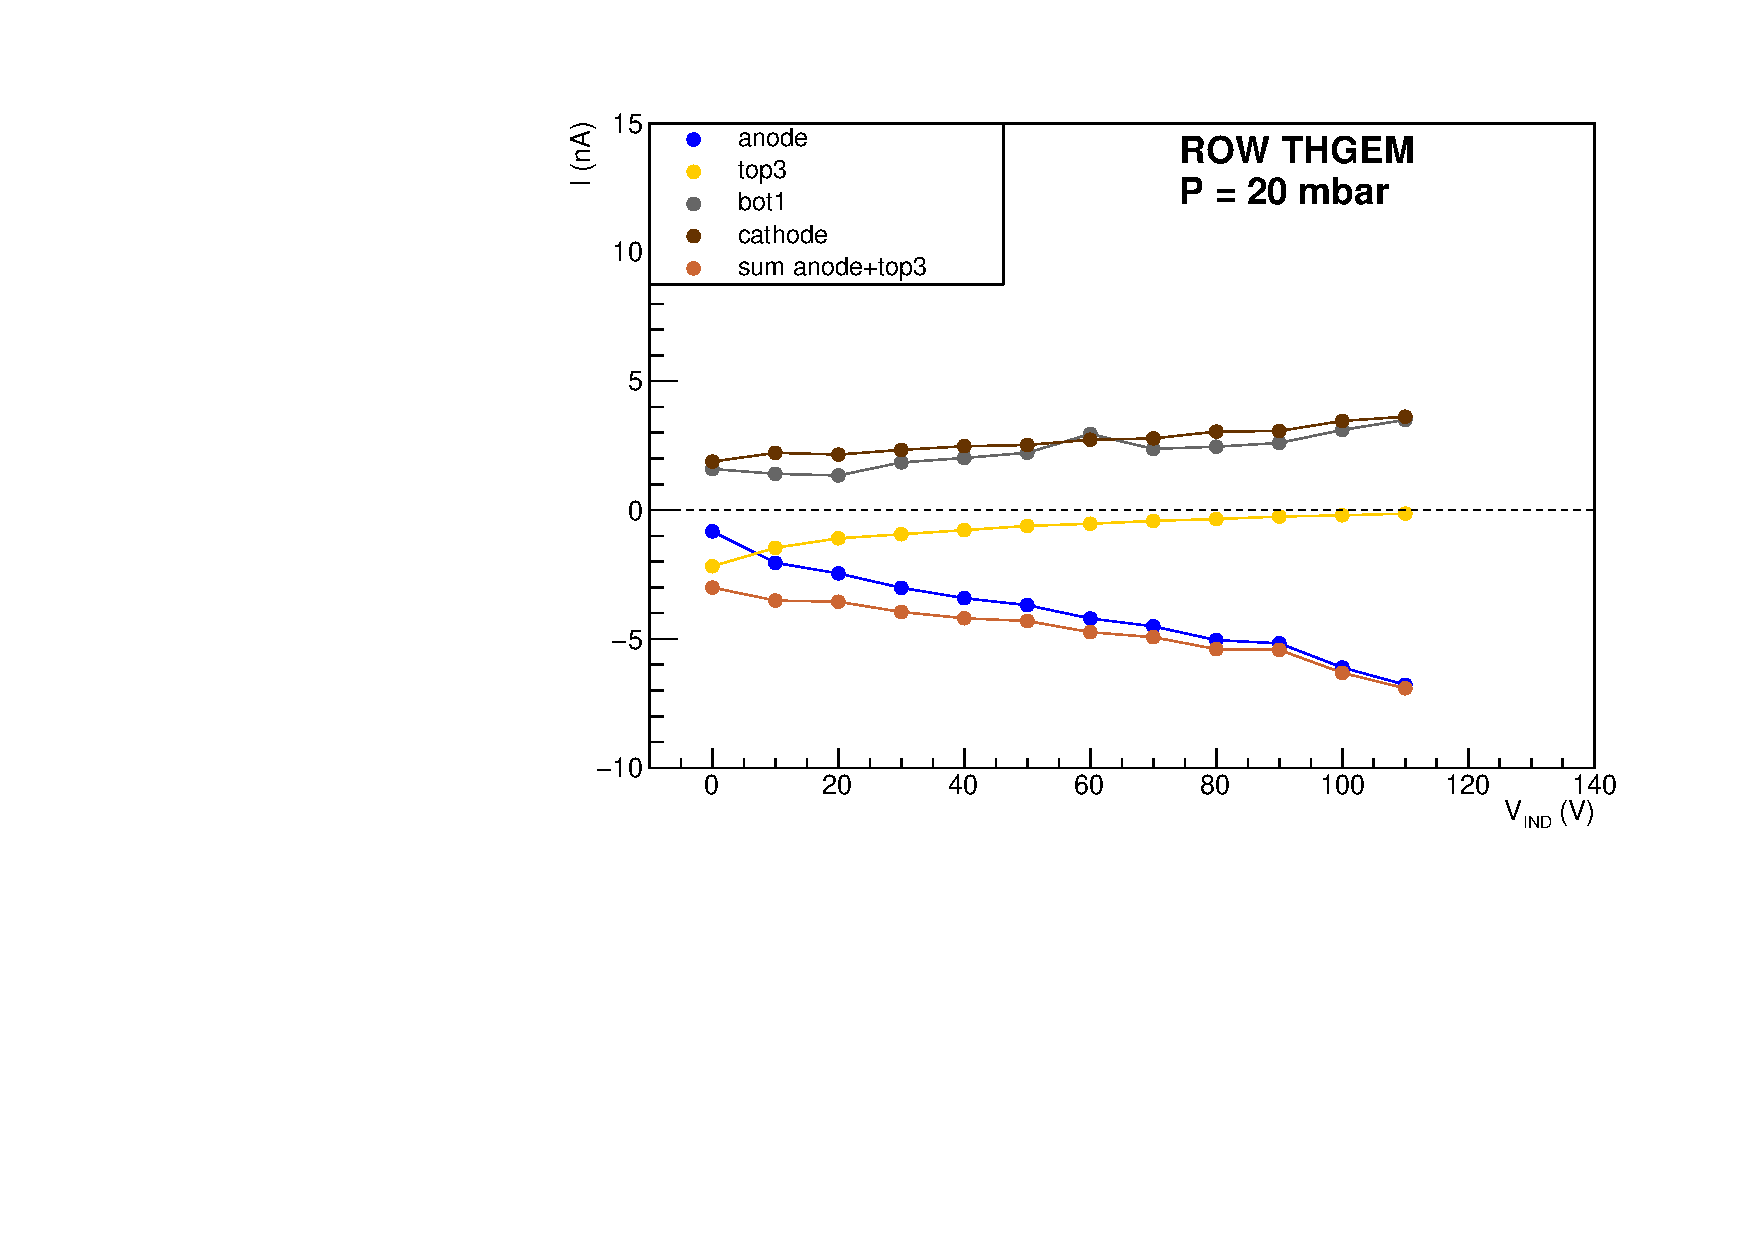
\includegraphics[width=0.96\textwidth]{Immagini/InductionScan_ROW_THGEM_20mbar.pdf}}
	\subfigure[]{ 	\label{fig:induction_ROWTHGEM_20mbar_bis} 
	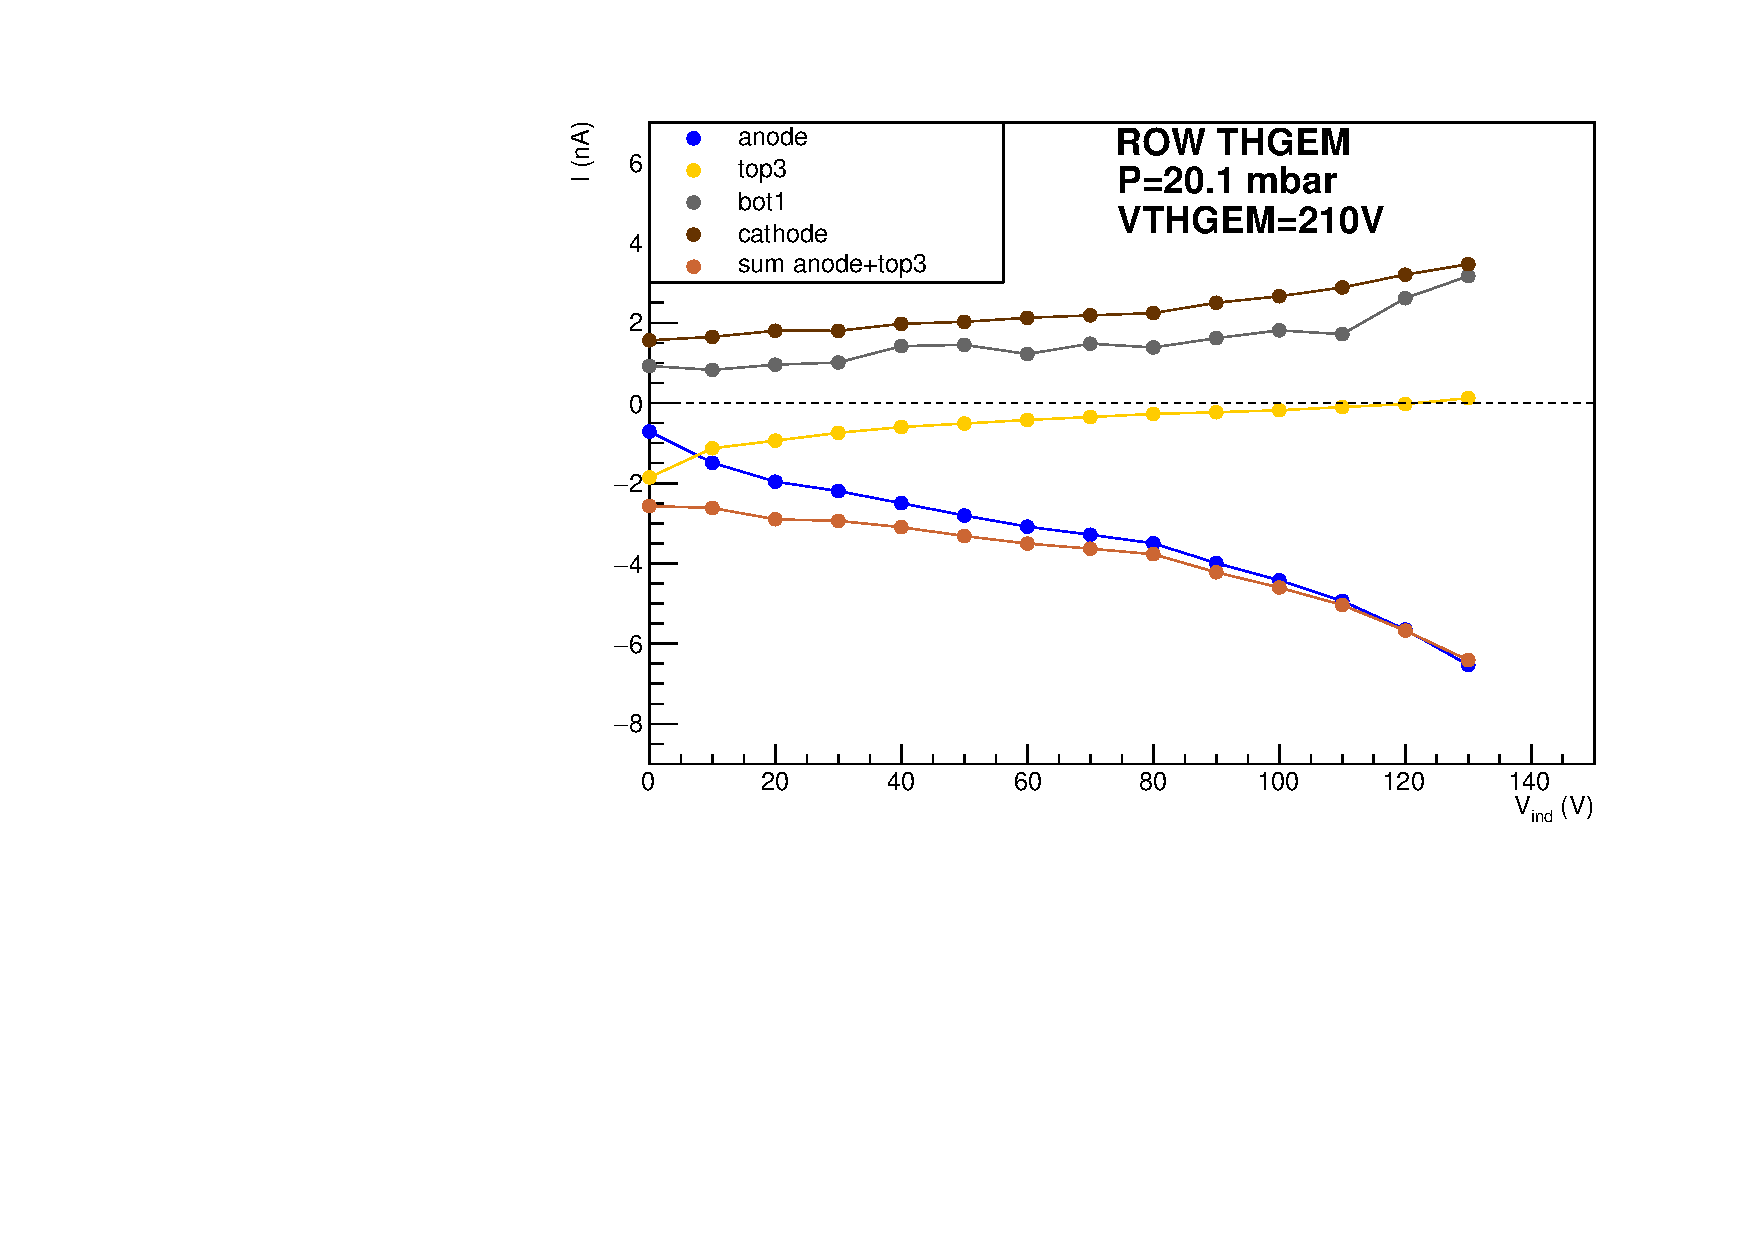
\includegraphics[width=0.96\textwidth]{Immagini/InductionScan_ROW_THGEM_20mbar_bis.pdf}}
	\caption{Currents measured during the scan on the voltage \Vind{} across the induction region at 
	20~mbar: in (a) \Vthgem{} is at 220~V, in (b) it is at 210~V.}
	\label{fig:induction_ROWTHGEM_20mbar_both}
\end{figure}
Little discharges were observed up to 50~V, while in the range 60$\div$110~V big discharges affected 
bot1 and top3 currents.  or the Row THGEM at 20 mbar we choose as operational value  50~V or 60~V.

The plot at 30 and 40~mbar are shown in Figure~\ref{fig:induction_ROWTHGEM_30mbar} and~\ref{fig:induction_ROWTHGEM_40mbar}, 
we choose operational values of \Vind= 90 and 60 respectively.

\begin{figure}[!htb]
	\centering
	\subfigure[]{ \label{fig:induction_ROWTHGEM_30mbar} 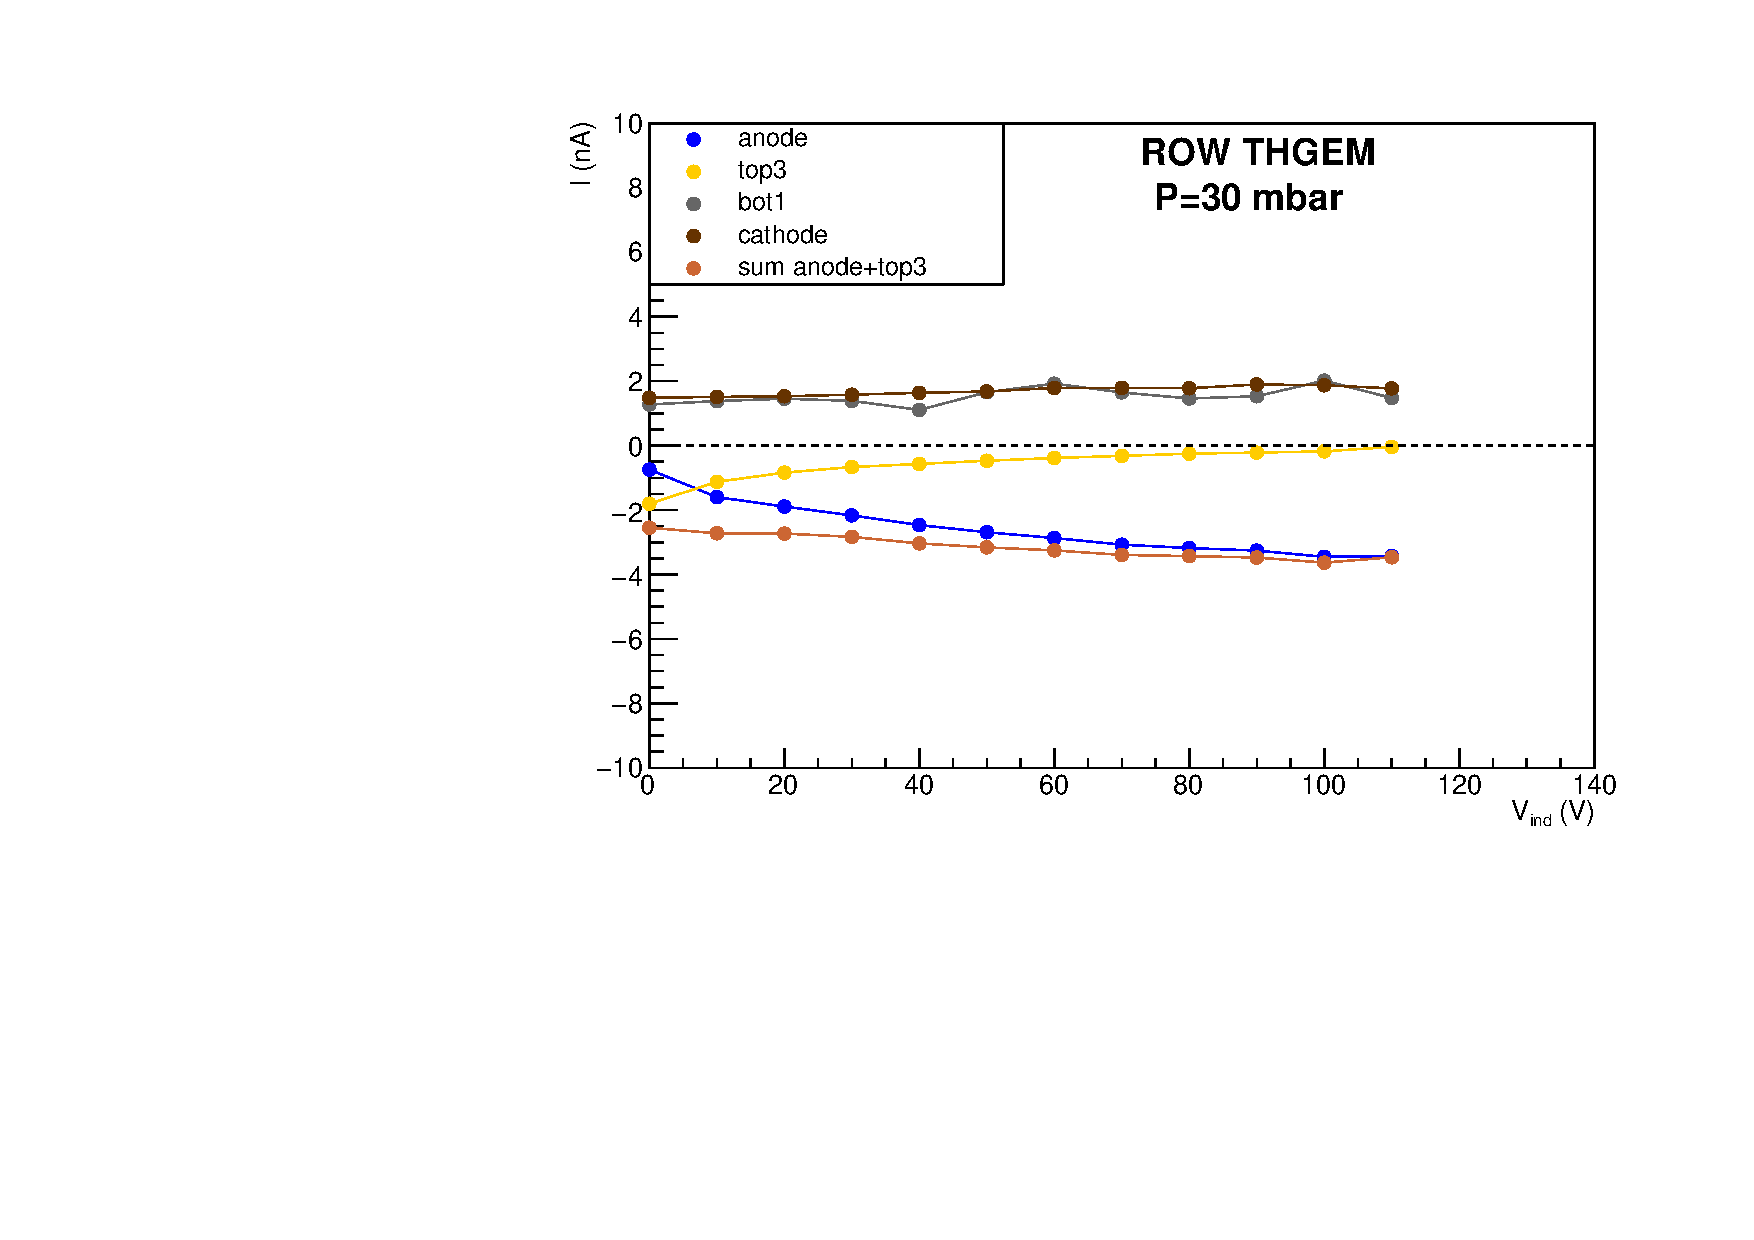
\includegraphics[width=0.96\textwidth]{Immagini/InductionScan_ROW_THGEM_30mbar.pdf}}
	\subfigure[]{ 	\label{fig:induction_ROWTHGEM_40mbar} 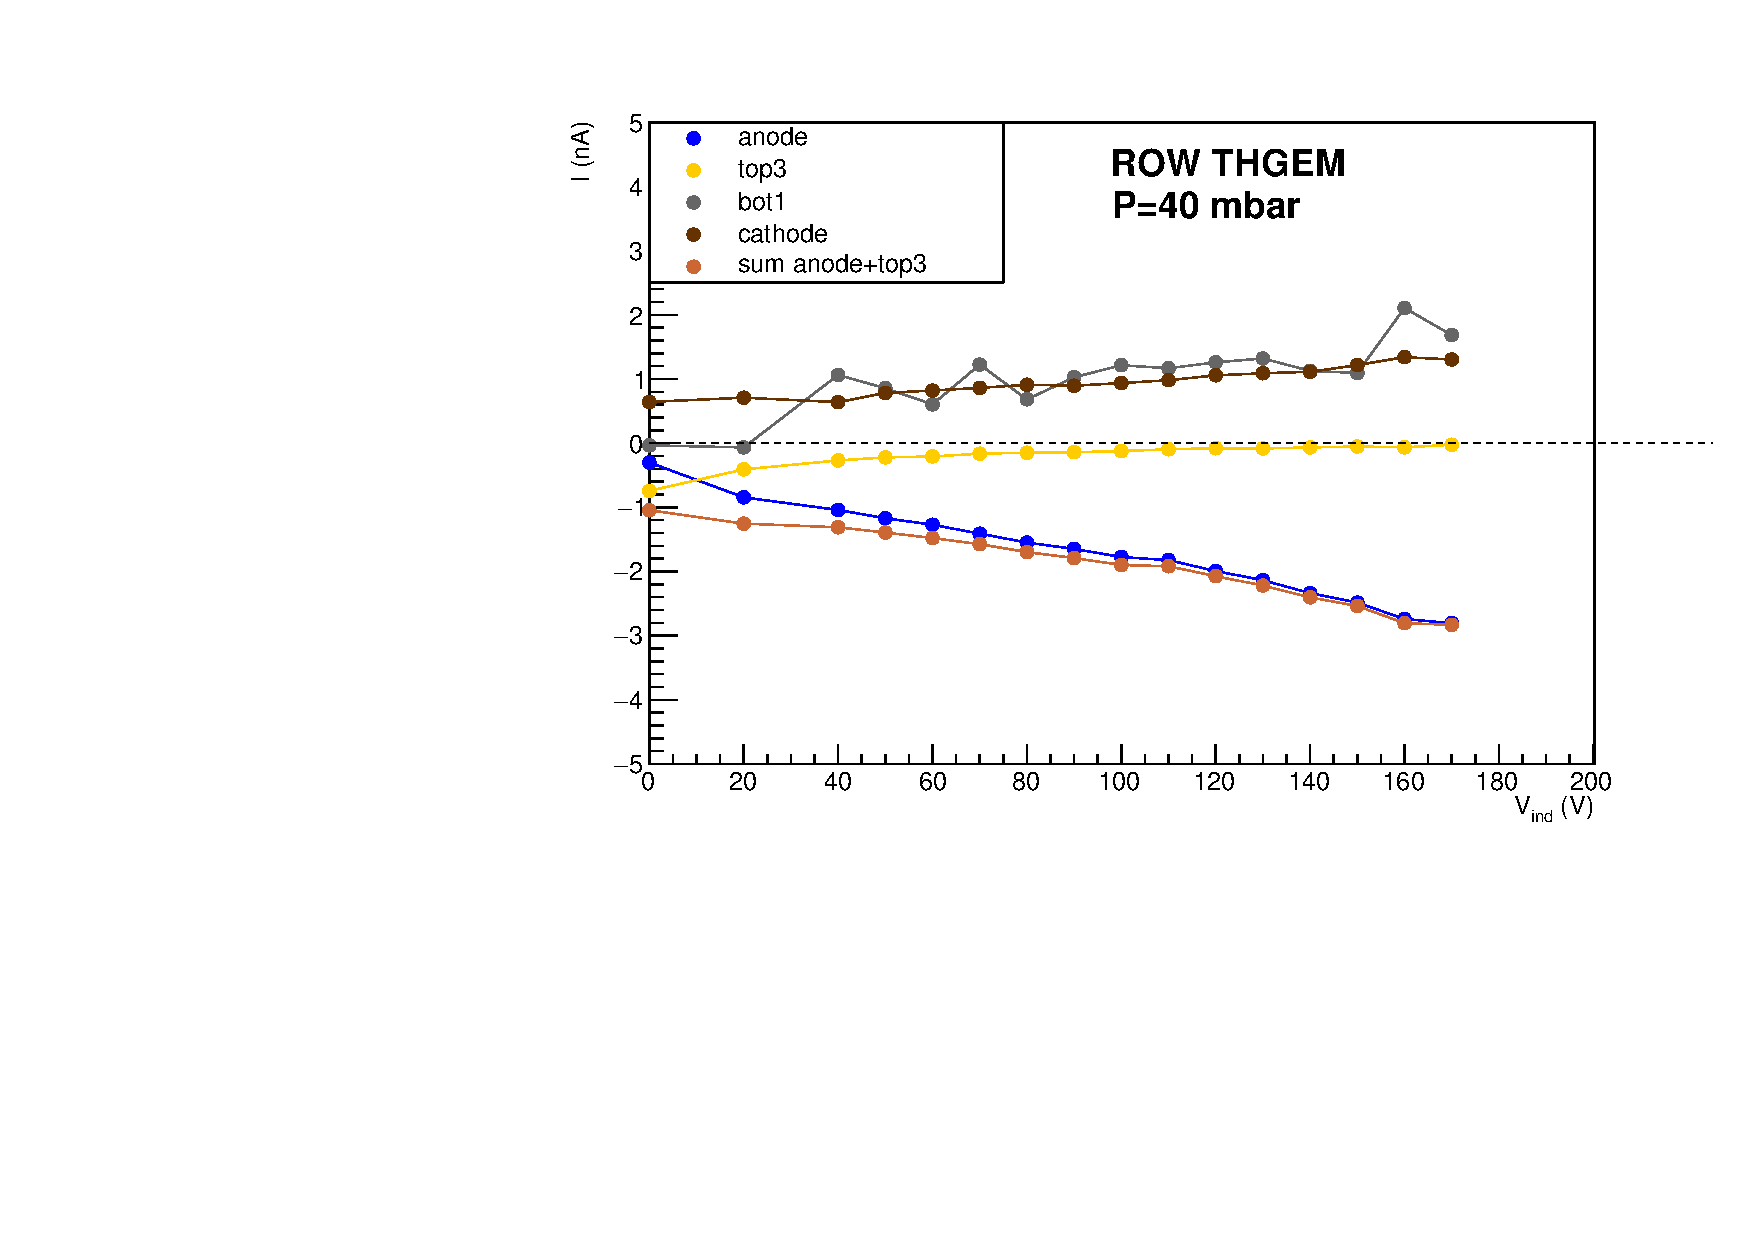
\includegraphics[width=0.96\textwidth]{Immagini/InductionScan_ROW_THGEM_40mbar.pdf}}
	\caption{Currents measured during the scan on the voltage \Vind{} across the induction region: in (a) at 30~mbar, in (b) at 40~mbar.}
	\label{fig:induction_ROWTHGEM_other_pressures}
\end{figure}
\clearpage


In Fig. \ref{fig:IBF_ALL_induction} the IBF as a function of \Vdrift is shown.
\begin{figure}[!htb]
	\centering
    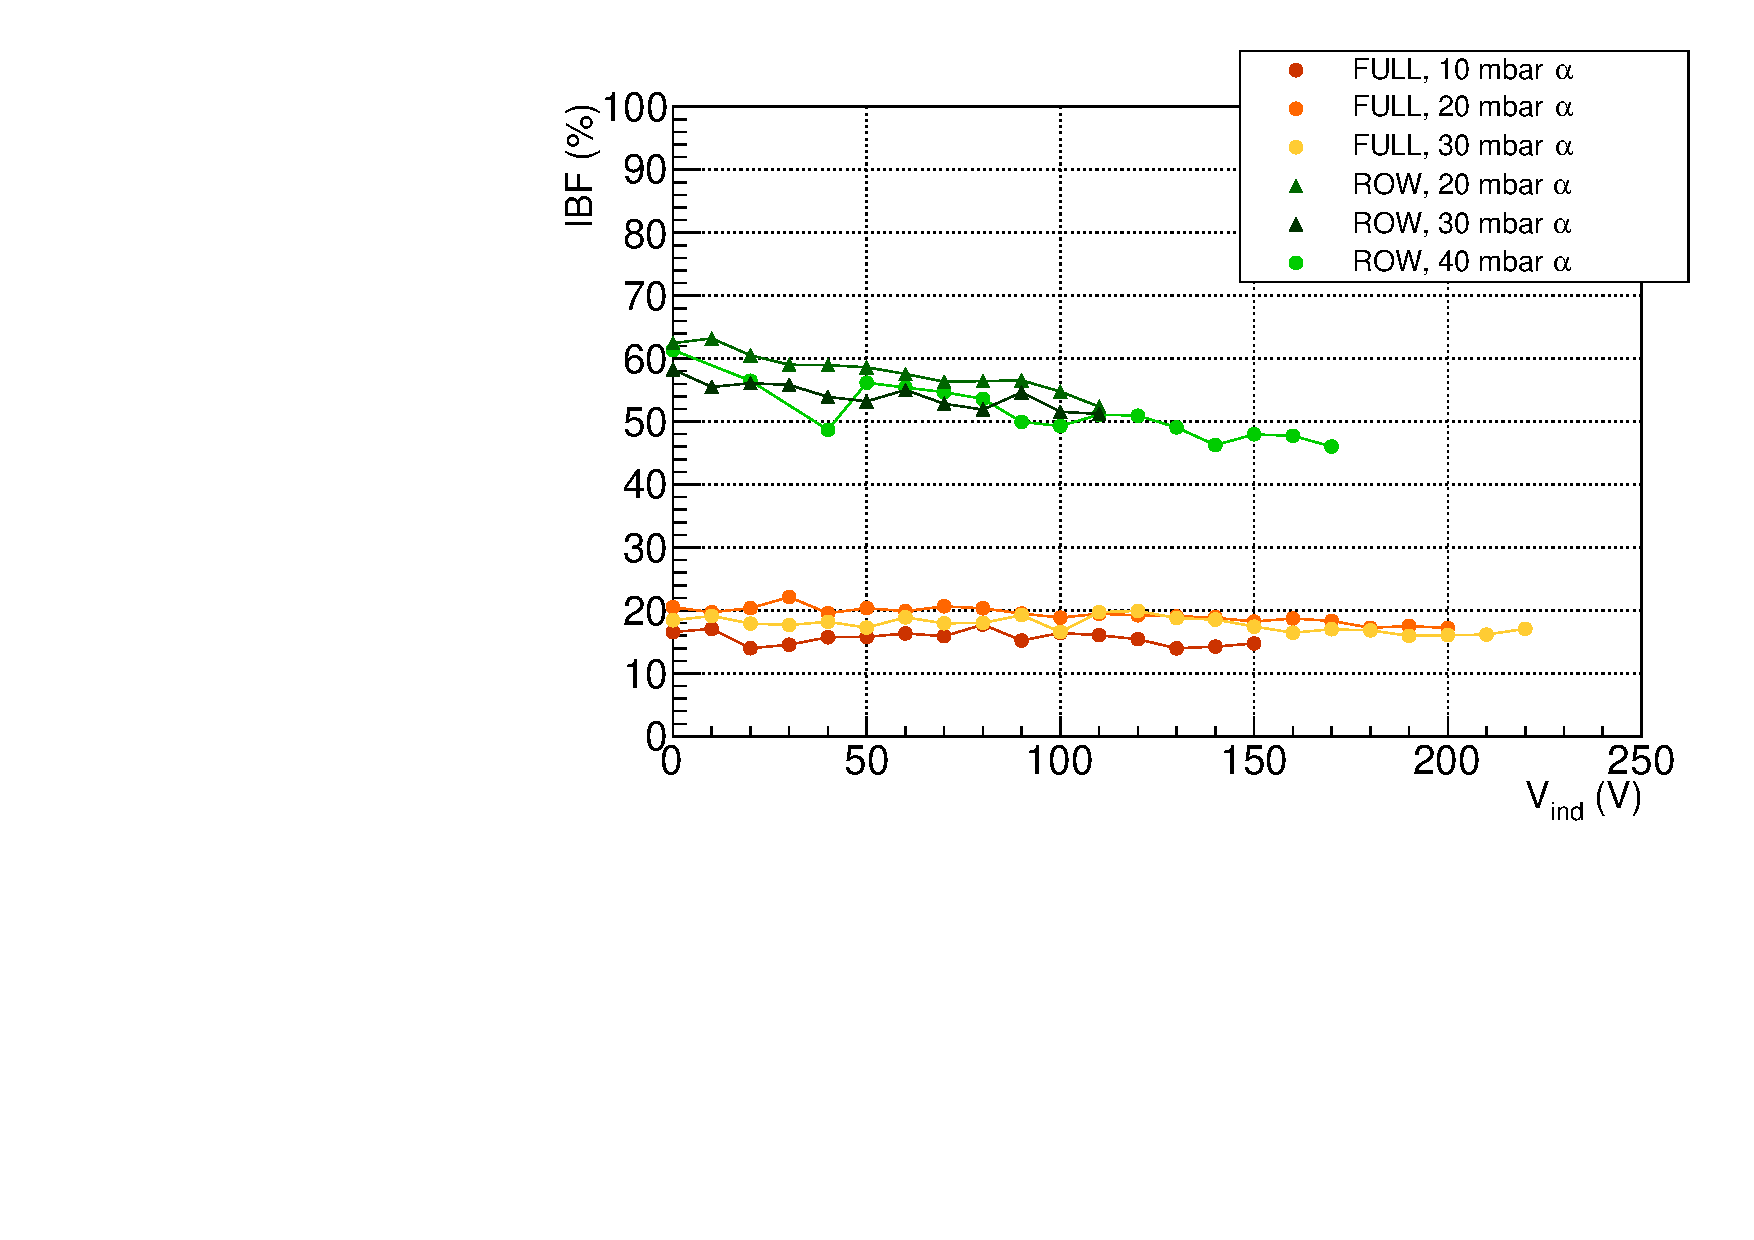
\includegraphics[width=0.96\textwidth]{Immagini/IBF_ALL_induction.pdf}
	\caption{IBF as a function of the voltage \Vind{} for FULL and ROW THGEM at different pressures.}
	\label{fig:IBF_ALL_induction}
\end{figure}




\subsubsection{Scan on \Vthgem}
The scan of \Vthgem have been done at fixed values of pressure, \Vind{} and \Vdrift{} and 
changing the \Vthgem at steps of 5/10~V.
A scheme of the different configuration used for the tes t is shown in Tab. \ref{tab:ROWTHGEM_vthgem}

\begin{table} [htbp]
	\begin{center}
		\renewcommand{\arraystretch}{1.2}
		\begin{tabular} {ccccccccc}
			P (mbar) & & \Vind{} (V) & & \Vdrift{} (V) & & \Vthgem{} range (V) & & run\\
			\toprule[0.1em]
			%\hline
			10		& & 50	& & 200	& & 140$\div$205 & & 342-352\\
			20.6	& &	50	& &	800 & & 180$\div$225 & & 227-232\\
			21.7	& & 80	& & 300	& & 120$\div$220 & & 323-341\\
			30		& &	70	& & 800 & & 180$\div$240 & & 260-267\\
			31.9	& & 70	& &	400	& & 170$\div$245 & & 309-322\\
			42		& & 80	& & 700 & & 220$\div$270 & & 300-308\\
			\bottomrule[0.1em]
		\end{tabular}
	\end{center}
	\caption{The values of pressure, \Vind{} and \Vdrift{} adopted for the study on \Vthgem{} and the 
	explored \Vthgem{} range.} \label{tab:ROWTHGEM_vthgem}
\end{table}
The scans at 10 and 32~mbar are shown, respectively, in Figure~\ref{fig:thgem_ROWTHGEM_10mbar} 
and~\ref{fig:thgem_ROWTHGEM_30mbar_bis}: Also in this case the currents follow an exponential law 
as a function of the increasing \Vthgem.
 
\begin{figure}[!htb]
	\centering
	\subfigure[]{ \label{fig:thgem_ROWTHGEM_10mbar} 
	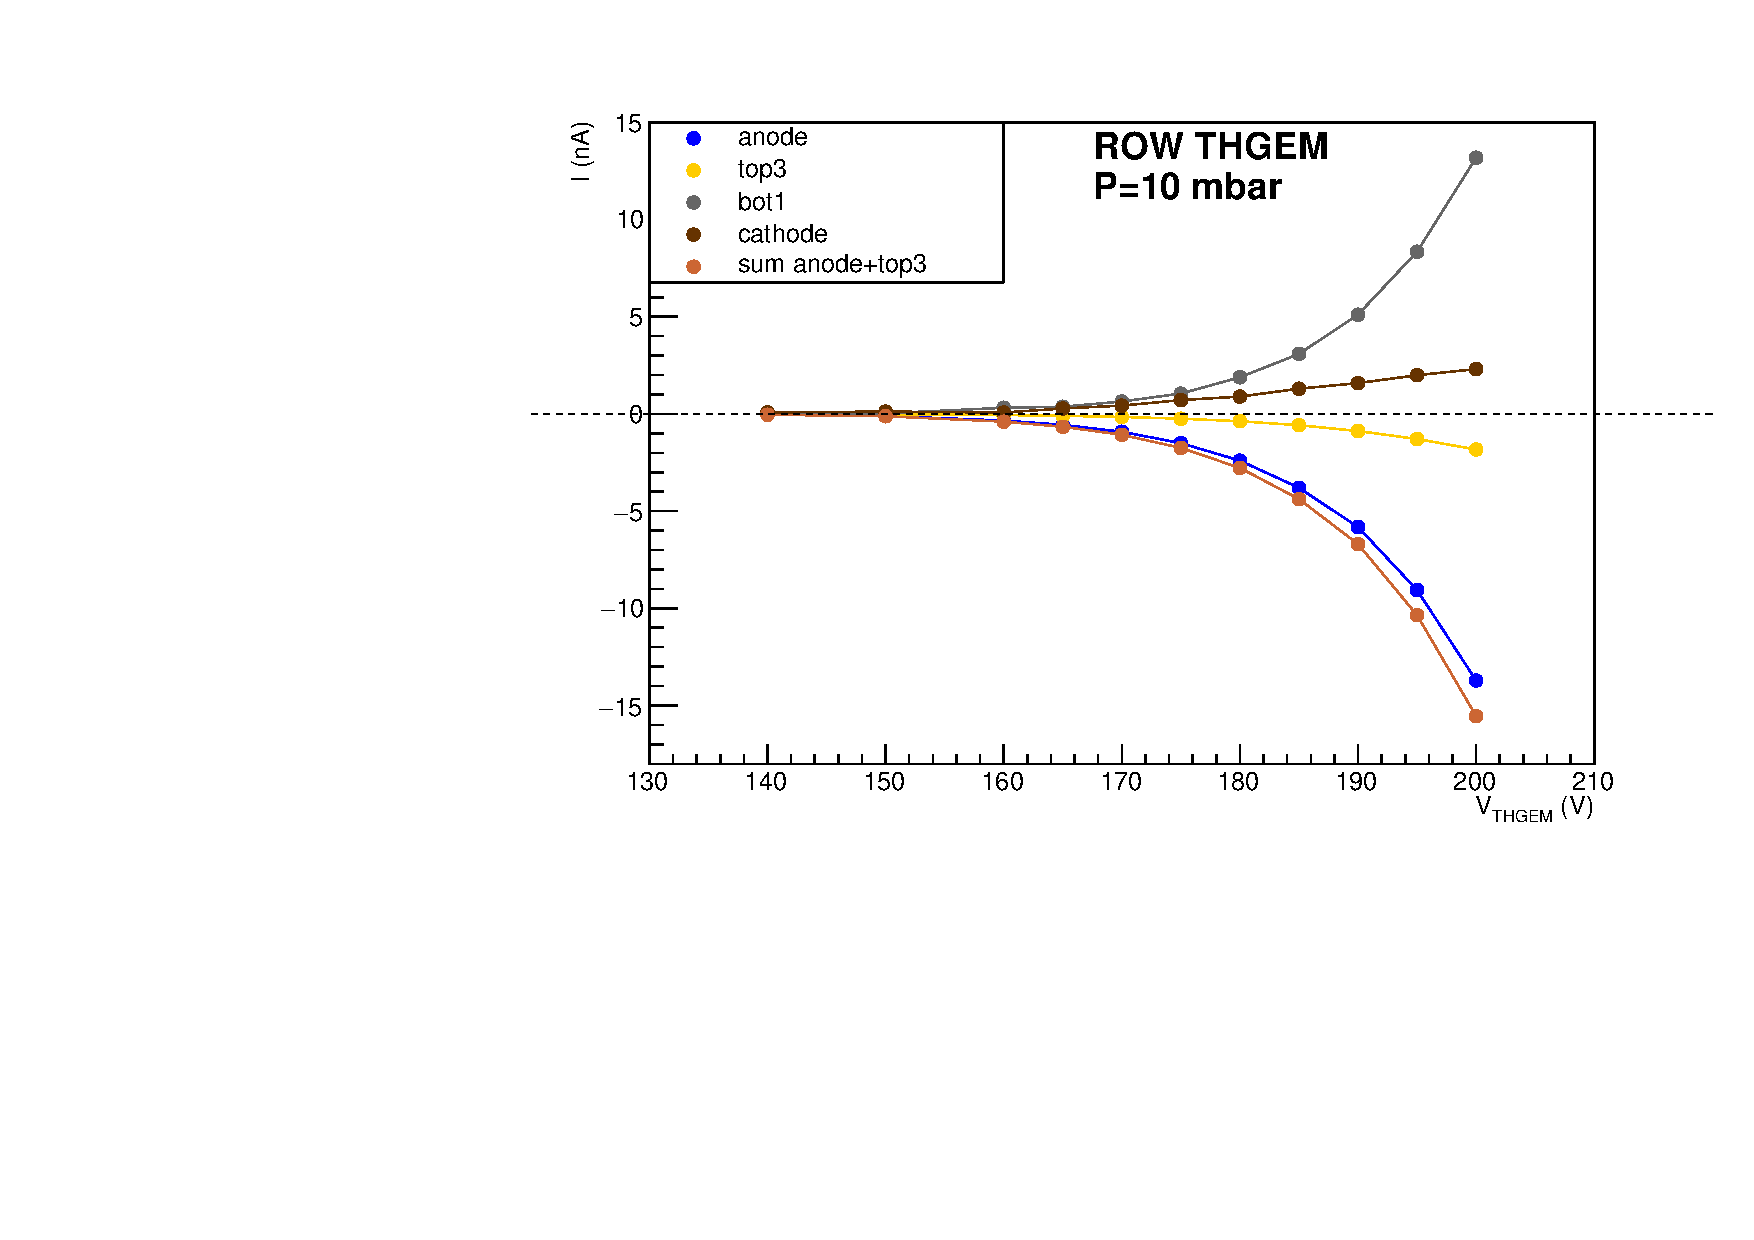
\includegraphics[width=0.96\textwidth]{Immagini/thgemScan_ROW_THGEM_10mbar.pdf}}
	\subfigure[]{ 	\label{fig:thgem_ROWTHGEM_30mbar_bis} 
	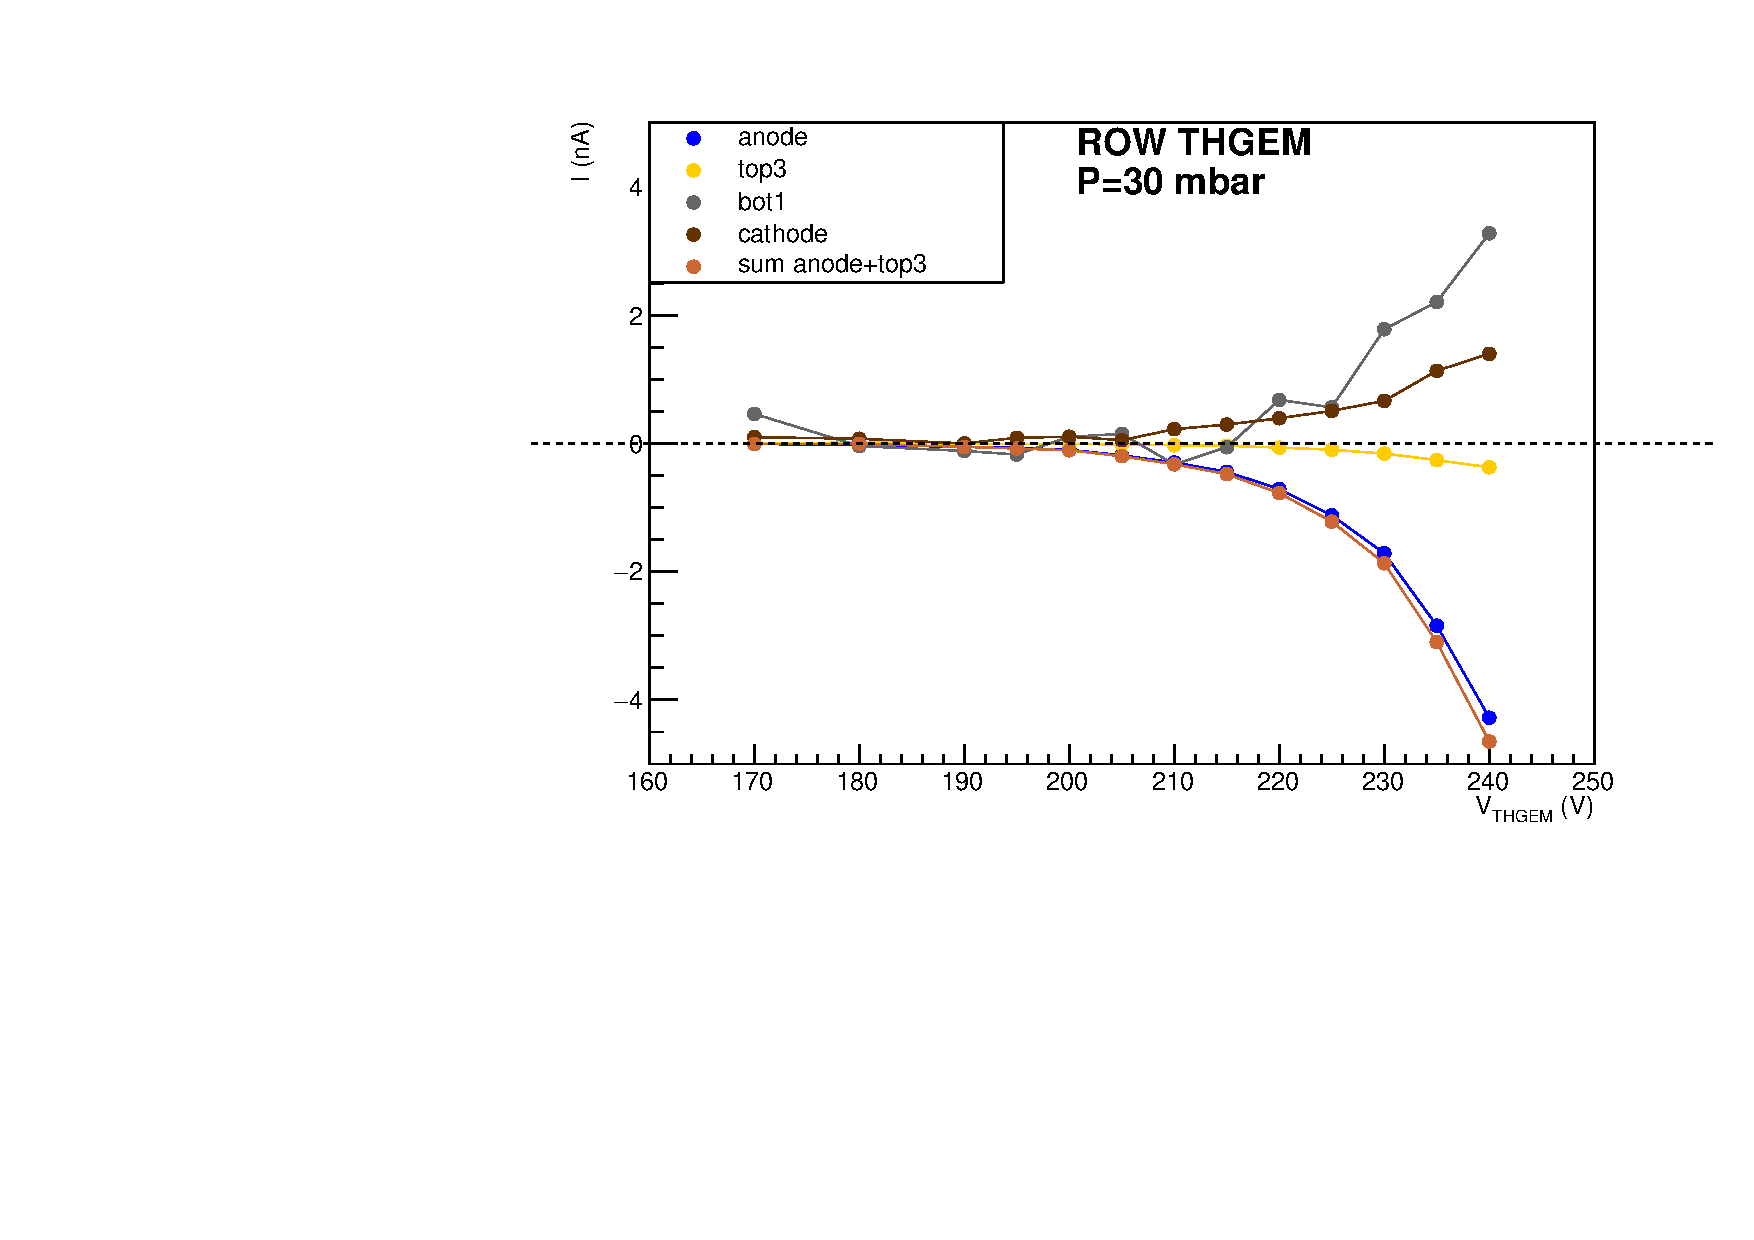
\includegraphics[width=0.96\textwidth]{Immagini/thgemScan_ROW_THGEM_30mbar_bis.pdf}}
	\caption{Currents measured during the scan on the voltage \Vthgem{} across each ROW THGEM: in (a)
	at 10~mbar, in (b) at 32~mbar.}
	\label{fig:thgem_ROWTHGEM}
\end{figure}

From these measurements, the multiplication factors of the ROW THGEM were evaluated as a function 
of \Vthgem{} and pressure Fig. \ref{fig:multiplication_factor_ROW}. Some clarification on the 
way the MF was measured is required. 
In fact due to the peculiar geometry of the ROW THGEM just a fraction of the primary elctrons
reach the holes while the remaining fraction of the electrons reach a inhert region of the 
THGEM. Therefore in order to correctly determine the multiplication factor we need to know the 
fraction of primary electrons that reach the holes.
Since we do not know this fraction we assume that it is 1. This assumptions has the effect 
to underestimate the MF.
\begin{figure}[!t]
	\centering
	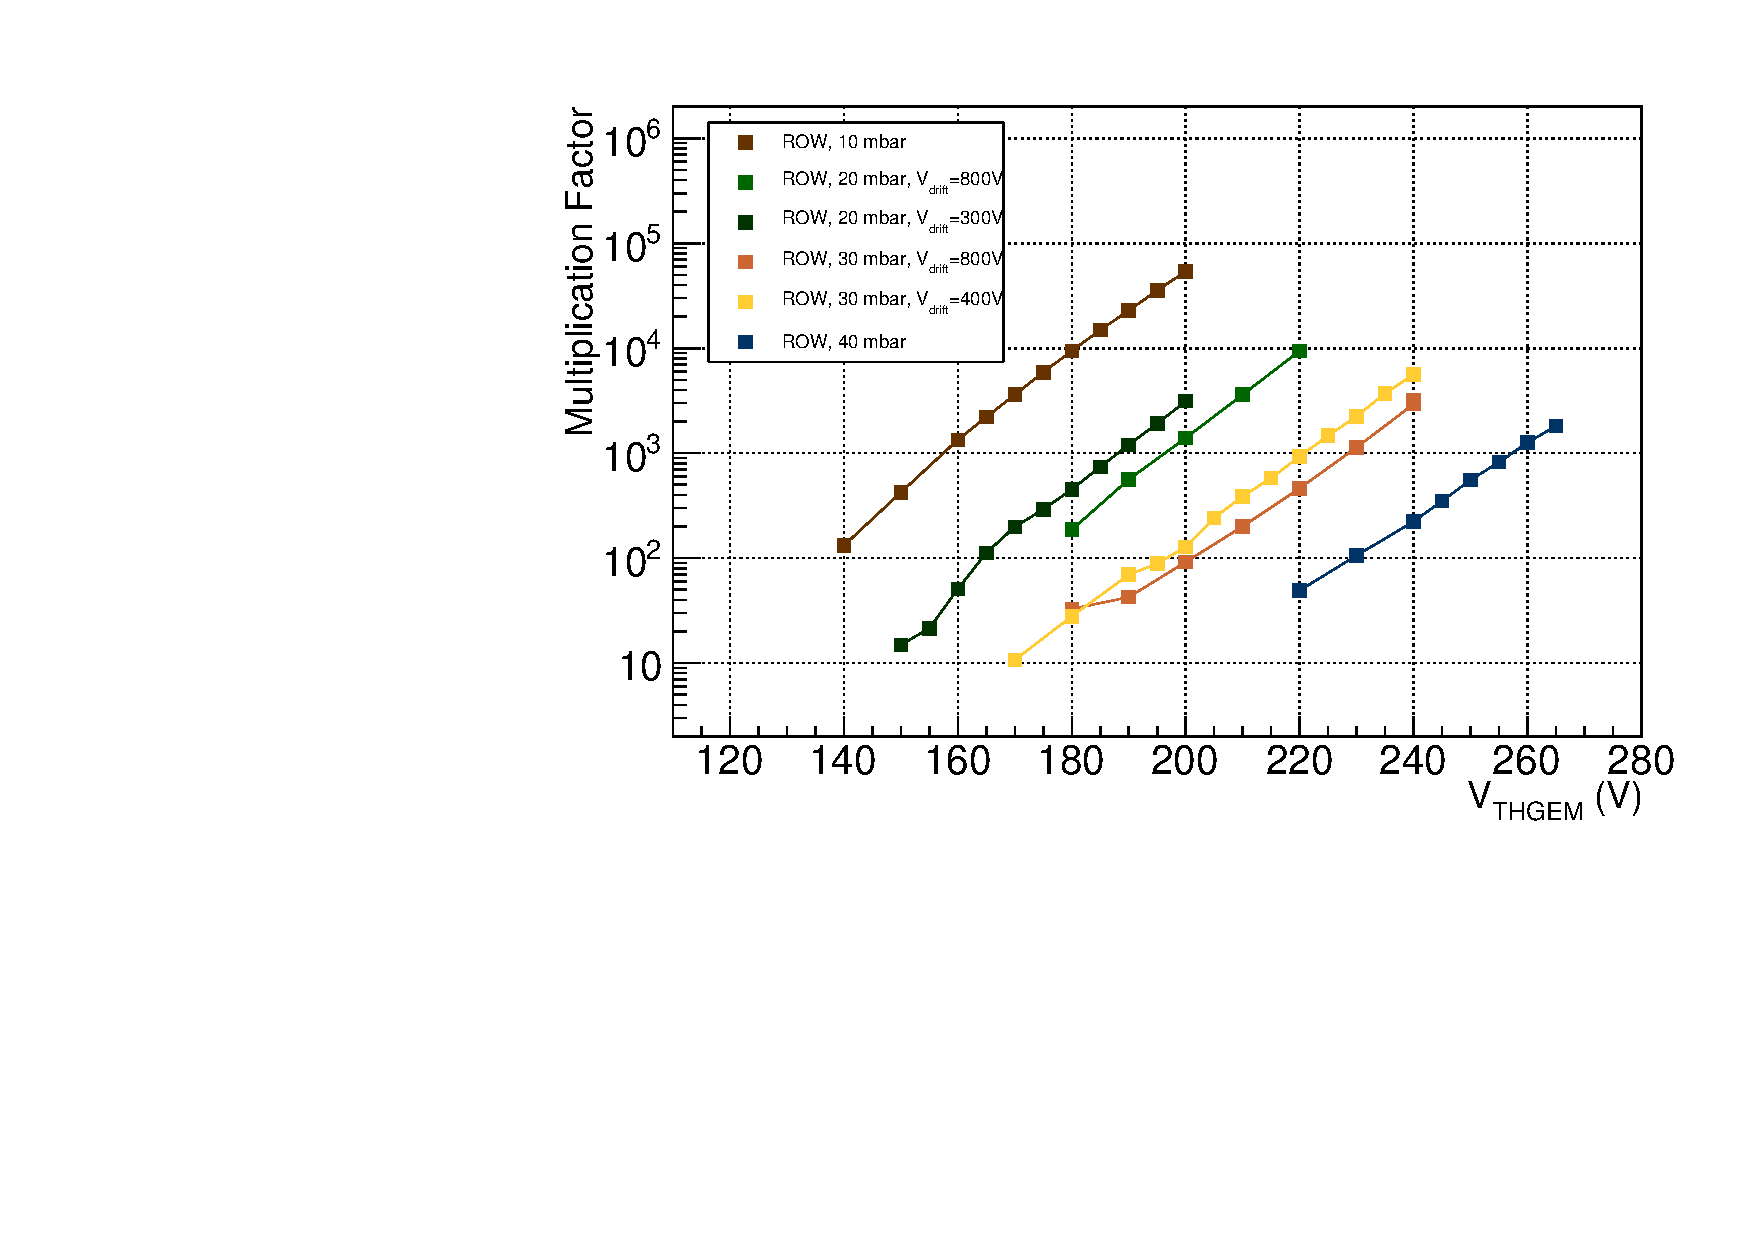
\includegraphics[width=\textwidth]{Immagini/MF_ROW_THGEM_noBeam.pdf}
	\caption{Multiplication factors evaluated for the ROW THGEM for different pressures.}
	\label{fig:multiplication_factor_ROW}
\end{figure}
In Fig. \ref{fig:multiplication_factor_FULLandROW} the comparison of the MF of the
two kind of THGEM is shown. As said before it is not possibe to make a direct
comparison between the two THGEM.

\begin{figure}[!t]
	\centering
	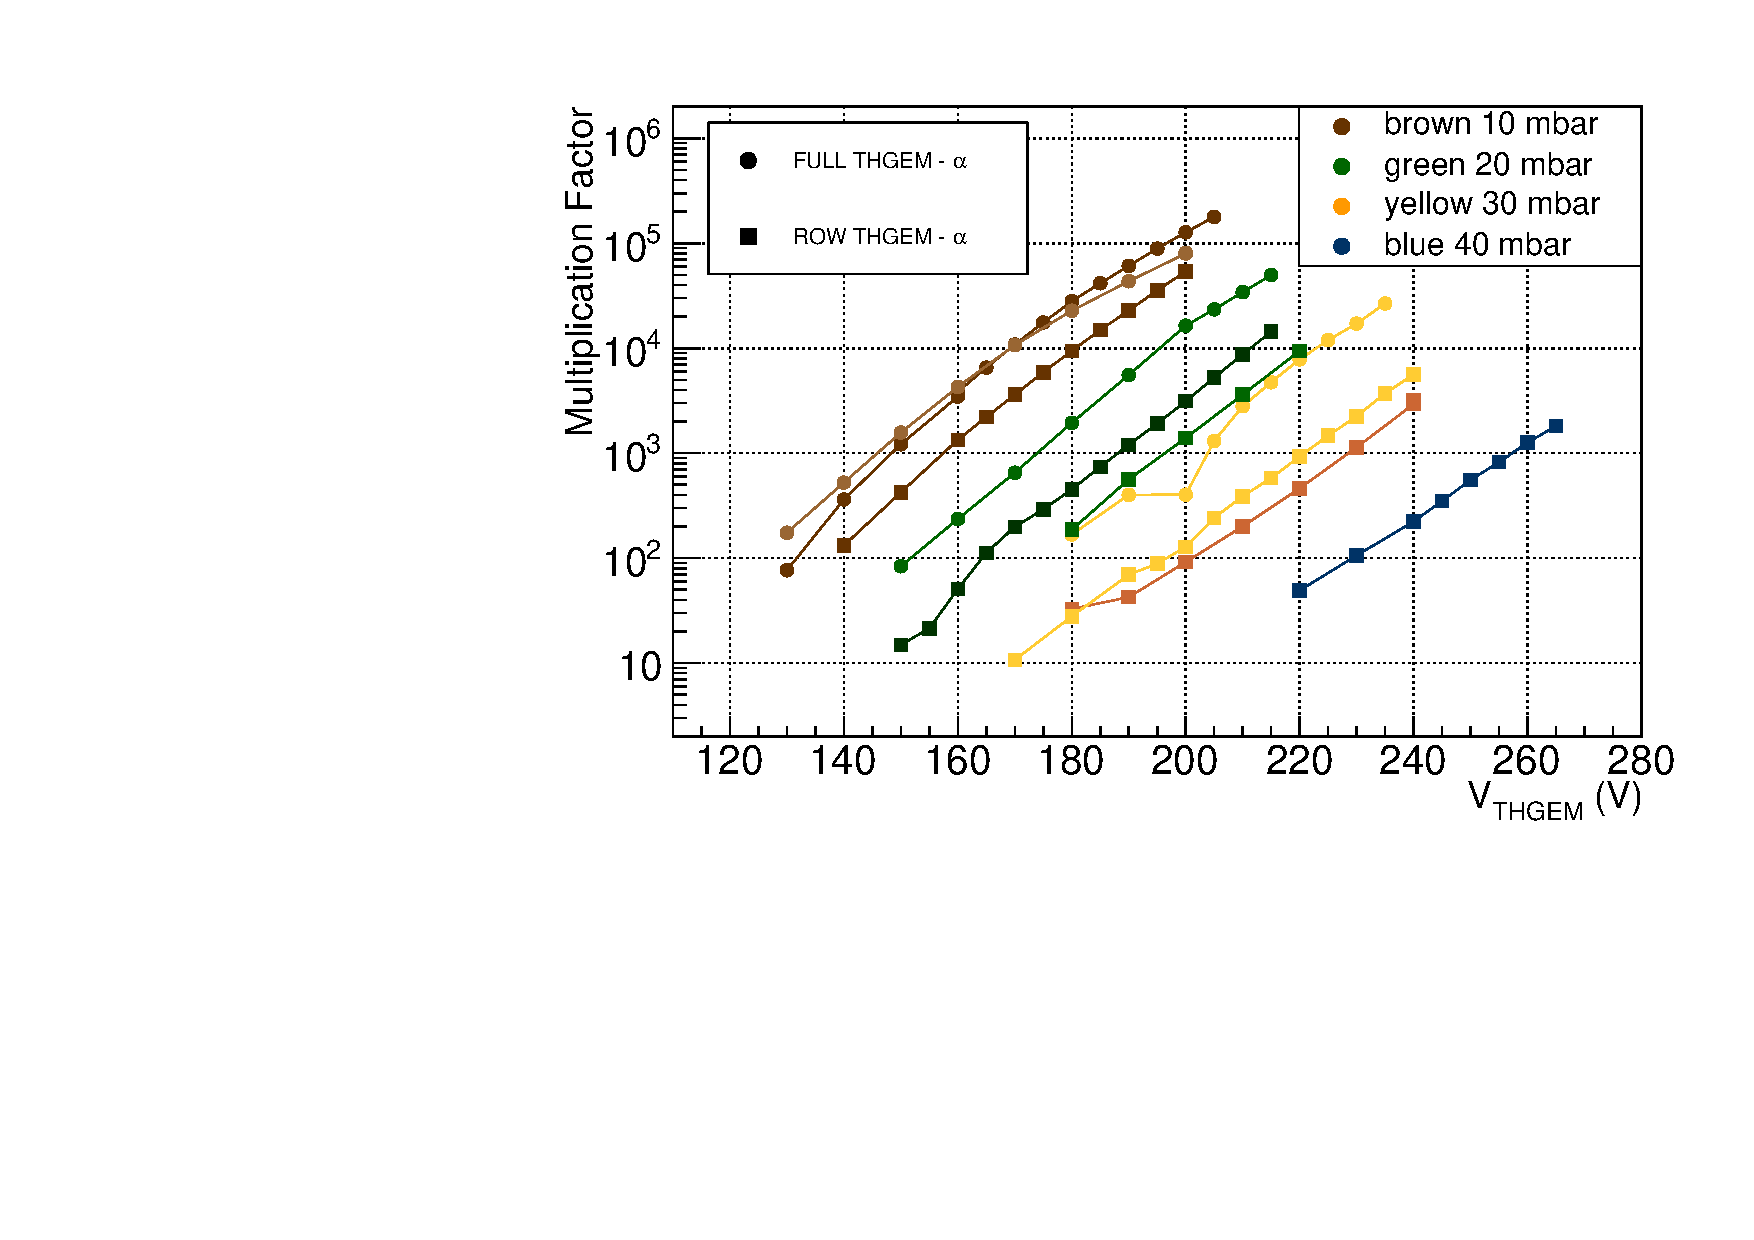
\includegraphics[width=\textwidth]{Immagini/MF_ALL_THGEM_noBeam.pdf}
	\caption{Comparison between the multiplication factors evaluated for the ROW THGEM (square) and 
	those for the FULL THGEM (circle) as a function of \Vthgem{} and pressure.}
	\label{fig:multiplication_factor_FULLandROW}
\end{figure}


\clearpage

\subsubsection{Scan on \Vdrift}
The scan of \Vdrift have been done at fixed values of pressure, \Vind{} and \Vthgem{}.
The explored range goes from 0~V\footnote{or 100~V in the case with P~=~20~mbar} to the discharge
voltage. A scheme of the different configuration used for the tes t is shown in Tab.
\ref{tab:ROWTHGEM_vdrift}
\begin{table} [!h]
	\begin{center}
		\renewcommand{\arraystretch}{1.2}
		\begin{tabular} {ccccccccc}
			P (mbar) & & \Vind{} (V) & & \Vthgem{} (V)& & \Vdrift & & run\\
			\toprule[0.1em]
			%\hline
			30		& &	70	& &	240 & & 0-1400 & & 245-259\\
			30		& &	70	& & 230 & & 0-1400 & & 268-282\\
			20.1	& & 80	& & 210 & & 100-1000 & & 354-363\\
			10		& & 50	& & 180 & & 0-800 & & 379-396\\
			\bottomrule[0.1em]
		\end{tabular}
	\end{center}
	\caption{The values of pressure (P), \Vind{} and \Vthgem{} adopted for the study on \Vdrift.} \label{tab:ROWTHGEM_vdrift}
\end{table}

The scan of the currents ceersus \Vdrift at 30~mbar are shown in Figure~\ref{fig:drift_ROWTHGEM_30mbar_both}.
The behaviour of the anodic e cathodic current is very peculiar. The currents initially 
increases\footnote{at \Vdrift=0 they are all 0, that is a different behaviour respect to the 
FullTHGEM.}, then reach a maximum value and then decrease again reaching a flat region. It is 
difficult to give a correct explanation of this bheaviour without a simulation of the electric 
field in the prototype. Anyway we can give a tentative and qualitative explanation. 
It is hardly difficult that this behaviour is due to a change of the multiplication factor of the 
THGEM since there is no evident reason why it should change so much and with different slopes 
increasing the \Vdrift. Most probably the effect is due to the fact that the change in \Vdrift, 
modify the shape of the electric field in the drift region and therefore change the fraction of the 
primary electron that reach the holes and are multiplied.\\
In fact the geometry of the Row THGEM make the electric field in the drift region not homogeneous 
since part of the field line that start from the cathode will be funneled in the hole while part of 
them will reach the inert region of the THGEM, i.e. that one without hole. Such ratio is modified 
by the applied \Vdrift therefore affecting the number for primary electron that reach the hole 
region and are effectively multiplied.
\begin{figure}[!htb]
	\centering
	\subfigure[]{ \label{fig:drift_ROWTHGEM_30mbar} 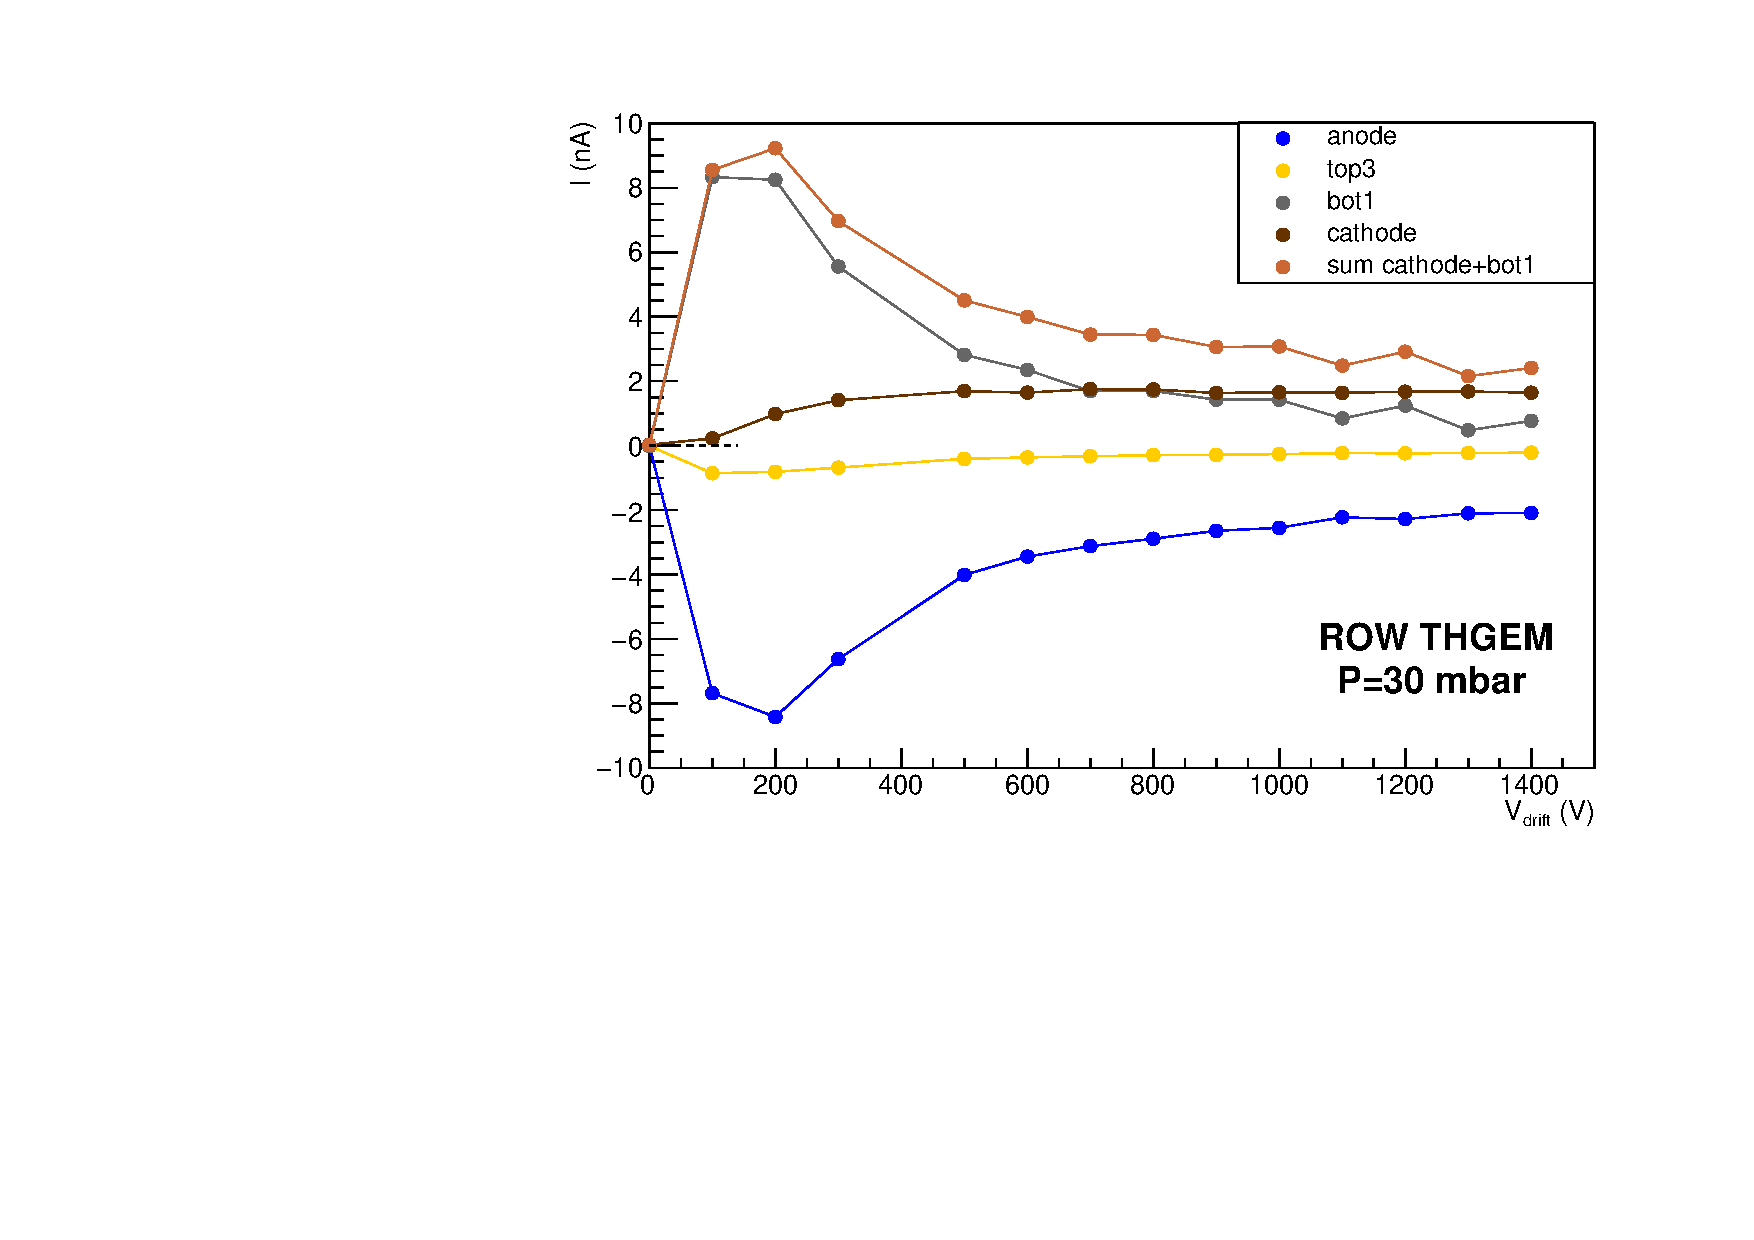
\includegraphics[width=0.96\textwidth]
	{Immagini/DriftScan_ROW_THGEM_30mbar.pdf}}
	\subfigure[]{ 	\label{fig:drift_ROWTHGEM_30mbar_bis} 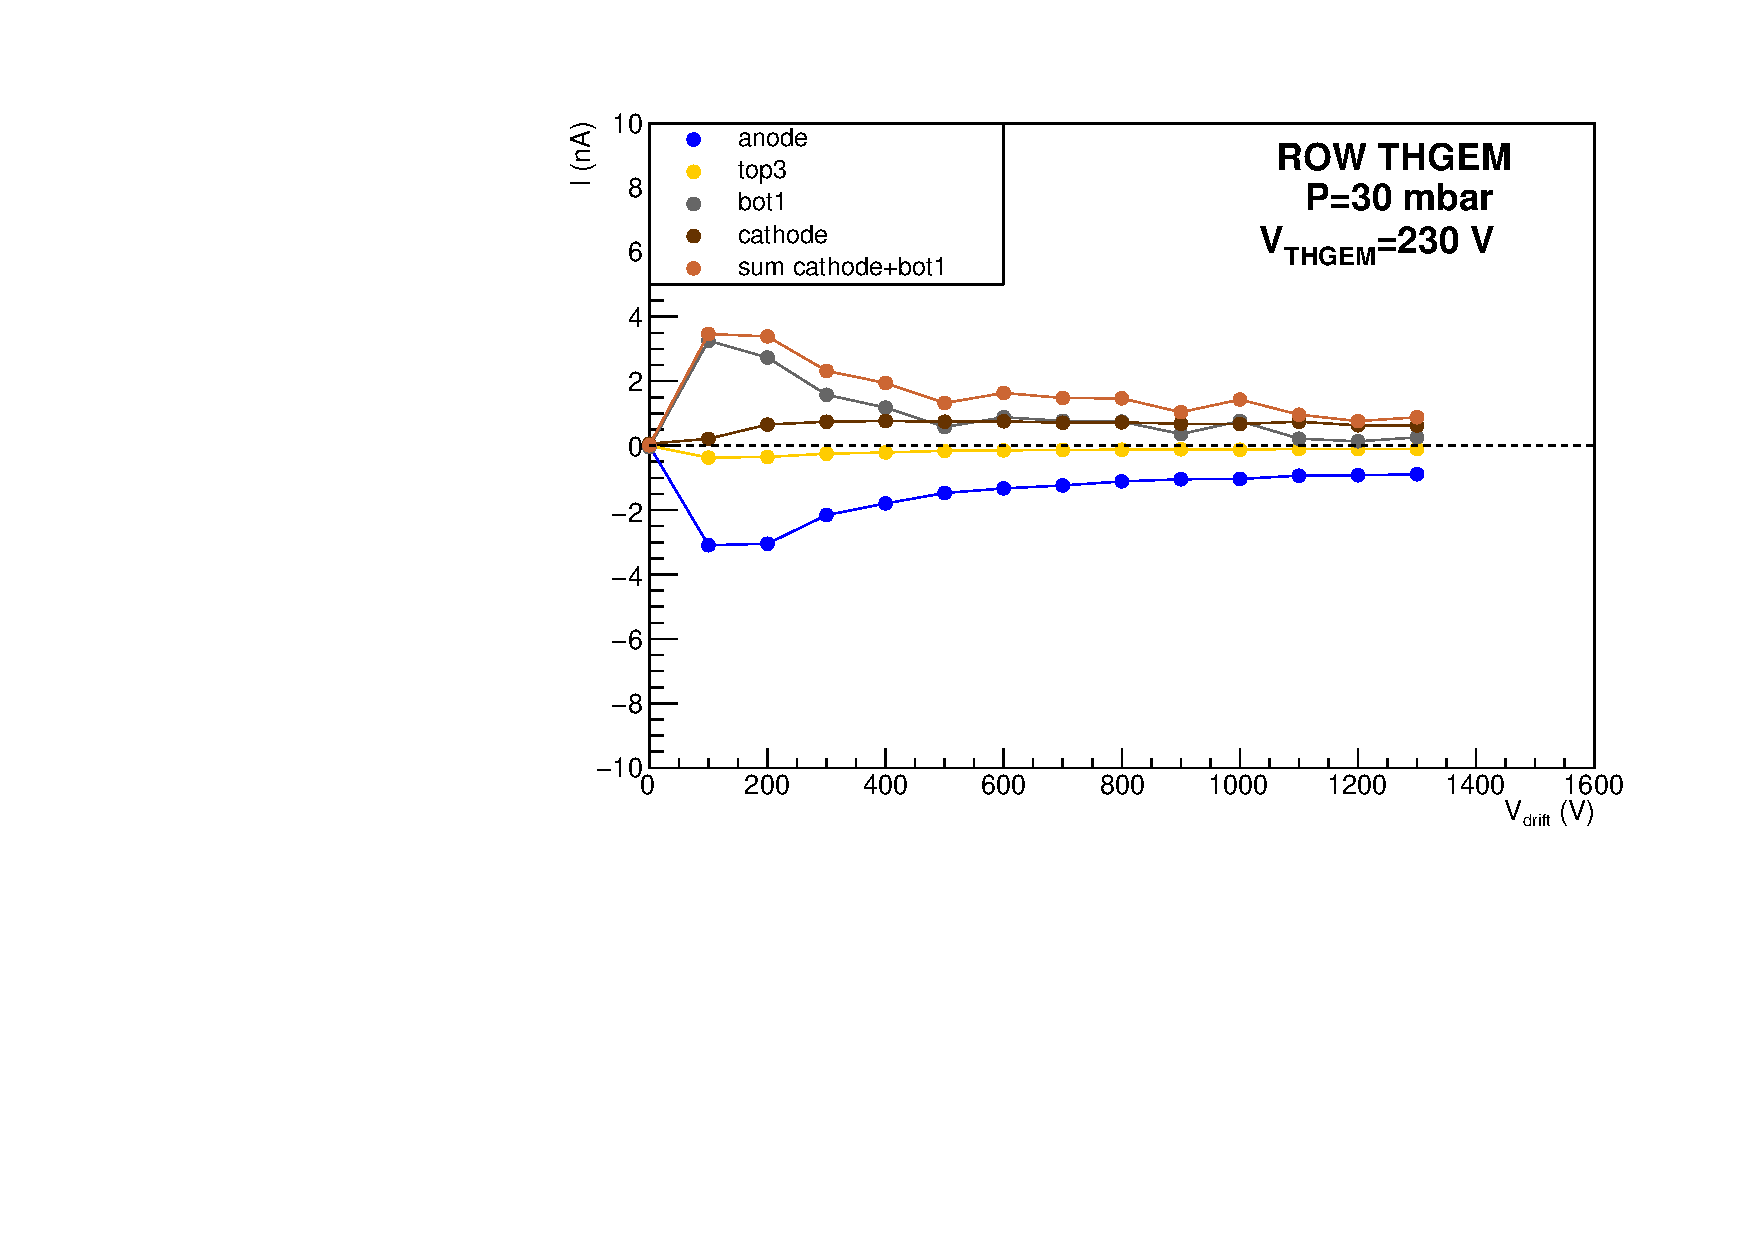
\includegraphics[width=0.96\textwidth]
	{Immagini/DriftScan_ROW_THGEM_30mbar_bis.pdf}}
	\caption{Currents measured during the scan on the voltage \Vdrift{} across the drift region at 
	20~mbar: in (a) \Vthgem{} is at 240~V, in (b) it is at 230~V.}
	\label{fig:drift_ROWTHGEM_30mbar_both}
\end{figure}
The same phenomenon appears also in the scans at 20 and 10~mbar, respectively shown in 
Figure~\ref{fig:drift_ROWTHGEM_20mbar} and~\ref{fig:drift_ROWTHGEM_10mbar}.
\begin{figure}[!htb]
	\centering
	\subfigure[]{ \label{fig:drift_ROWTHGEM_20mbar} 
	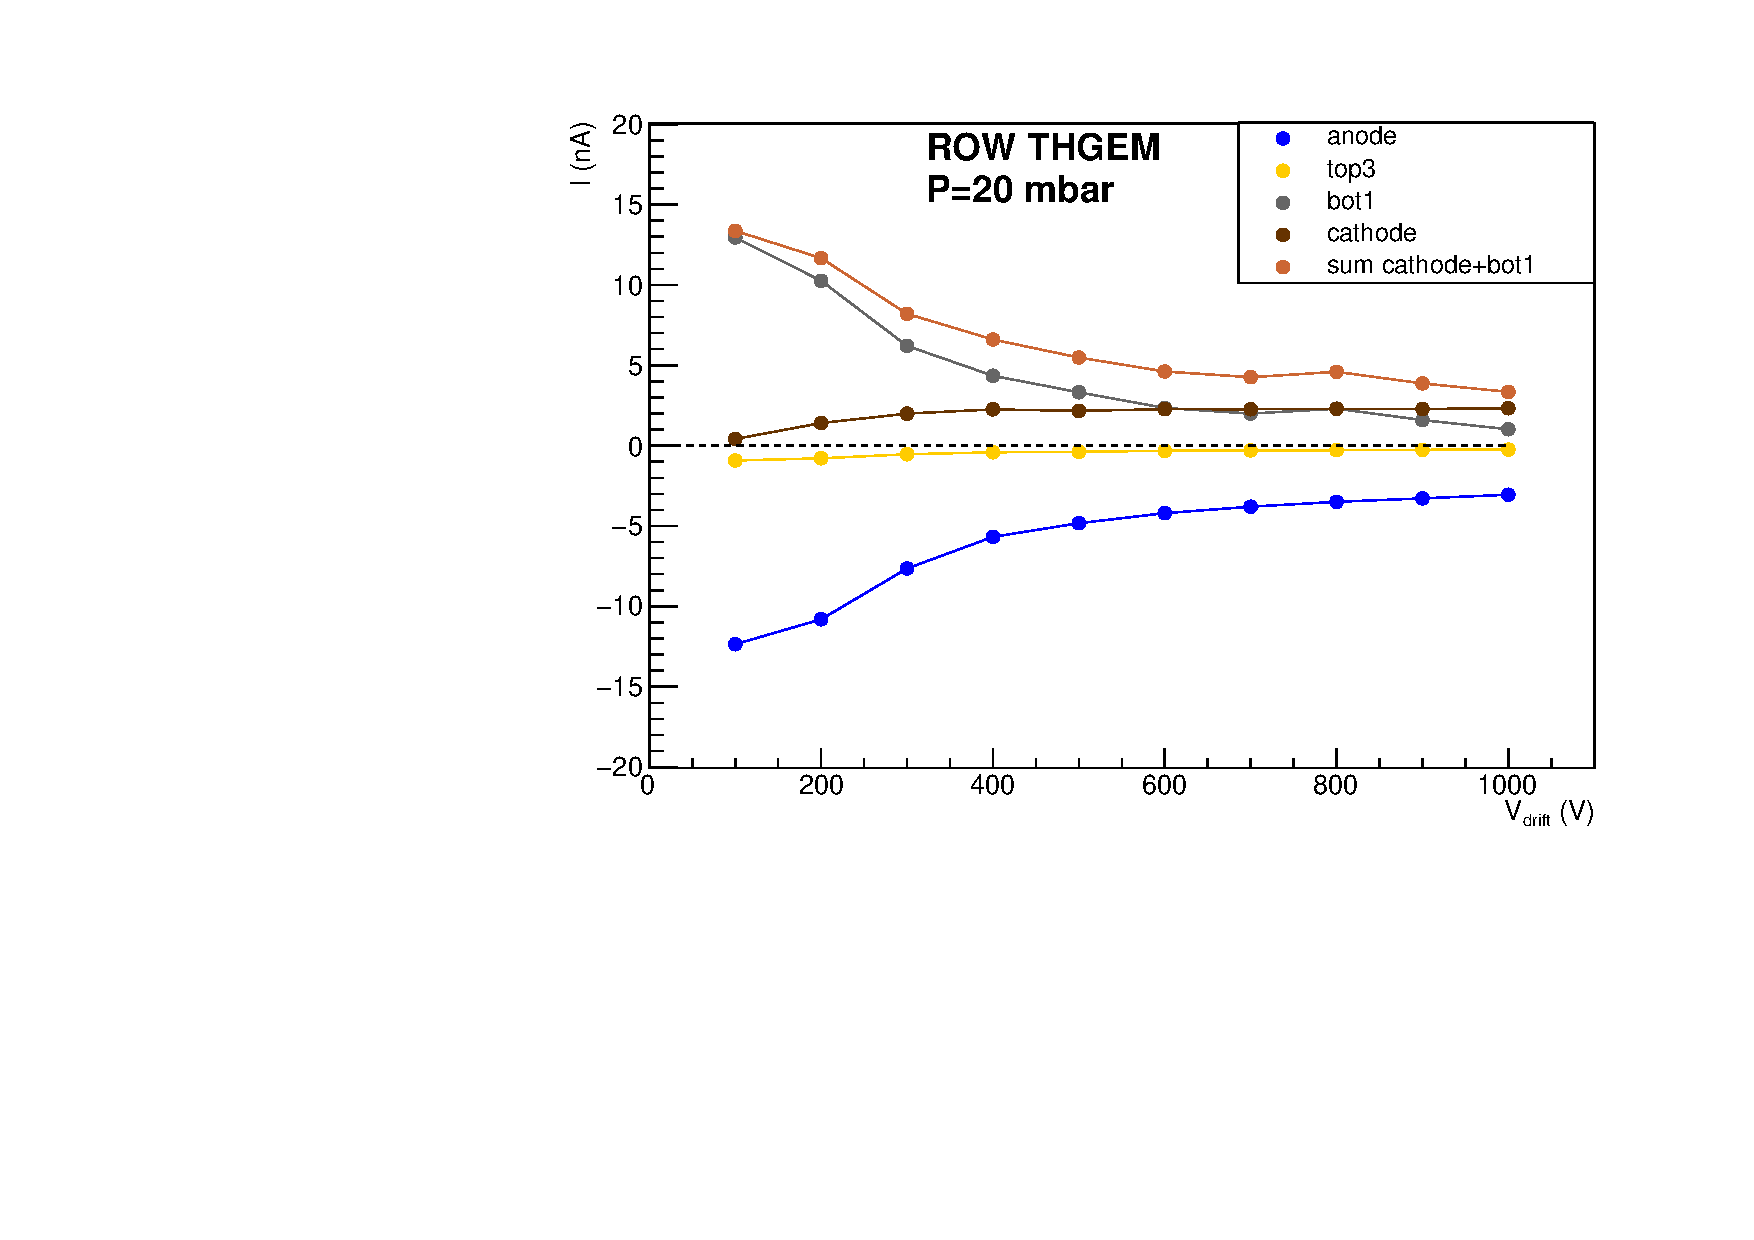
\includegraphics[width=0.96\textwidth]{Immagini/DriftScan_ROW_THGEM_20mbar.pdf}}
	\subfigure[]{ 	\label{fig:drift_ROWTHGEM_10mbar} 
	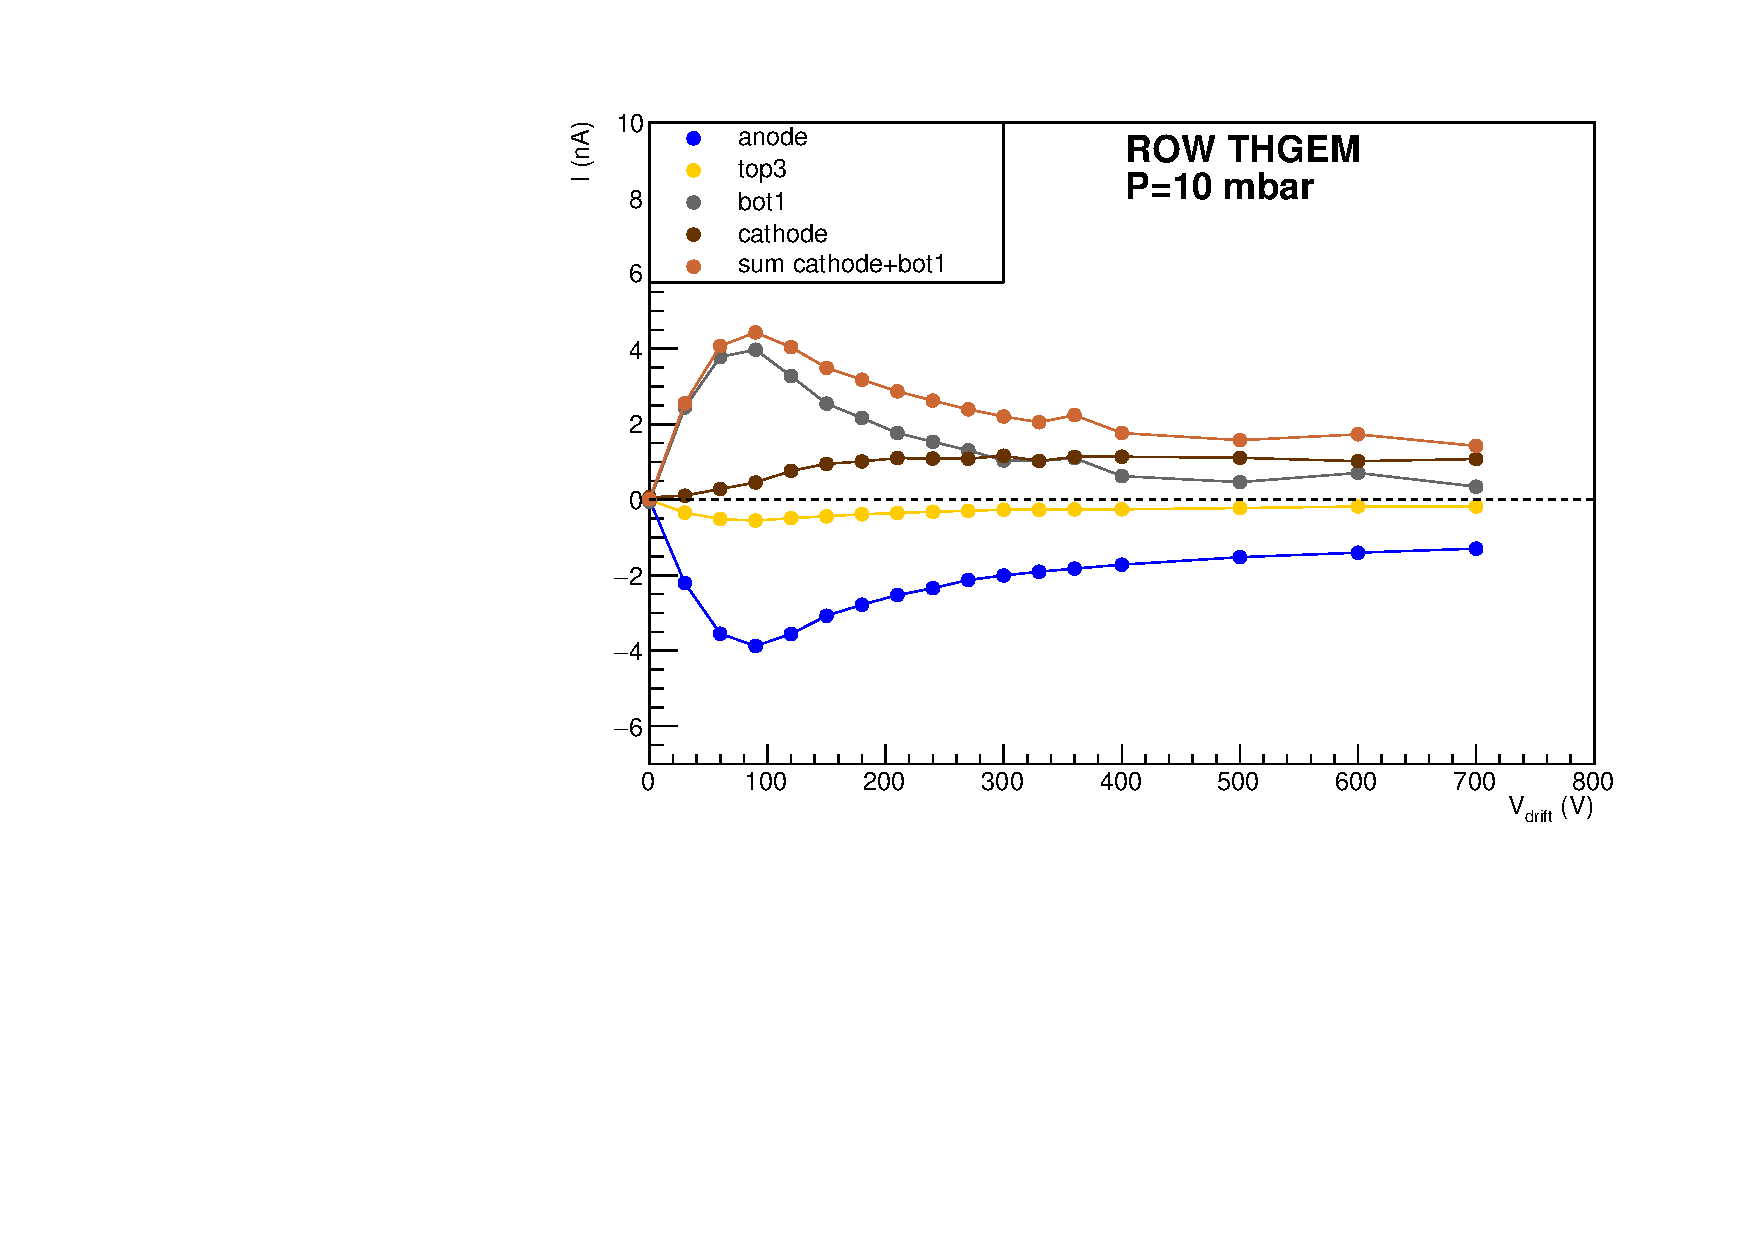
\includegraphics[width=0.96\textwidth]{Immagini/DriftScan_ROW_THGEM_10mbar.pdf}}
	\caption{Currents measured during the scan on the voltage \Vdrift{} across the drift region: in 
	(a) at 20~mbar, in (b) at 10~mbar.}
	\label{fig:drift_ROWTHGEM_20and10_mbar}
\end{figure}
From these measurements, the ion backflow of the ROW THGEM was evaluated as a function of \Vdrift{} 
for different pressures. The IBFs are shown in Figure~\ref{fig:ion_backflow_FULLandROW}.
In the same figure are shown for comparison also the IBF calculated for the Full THGEM.
It is evident that the IBF of the Row THGEM is much higher than that of the Full THGEM reaching 
values above 70\%.
\begin{figure}[htbp]
	\centering
	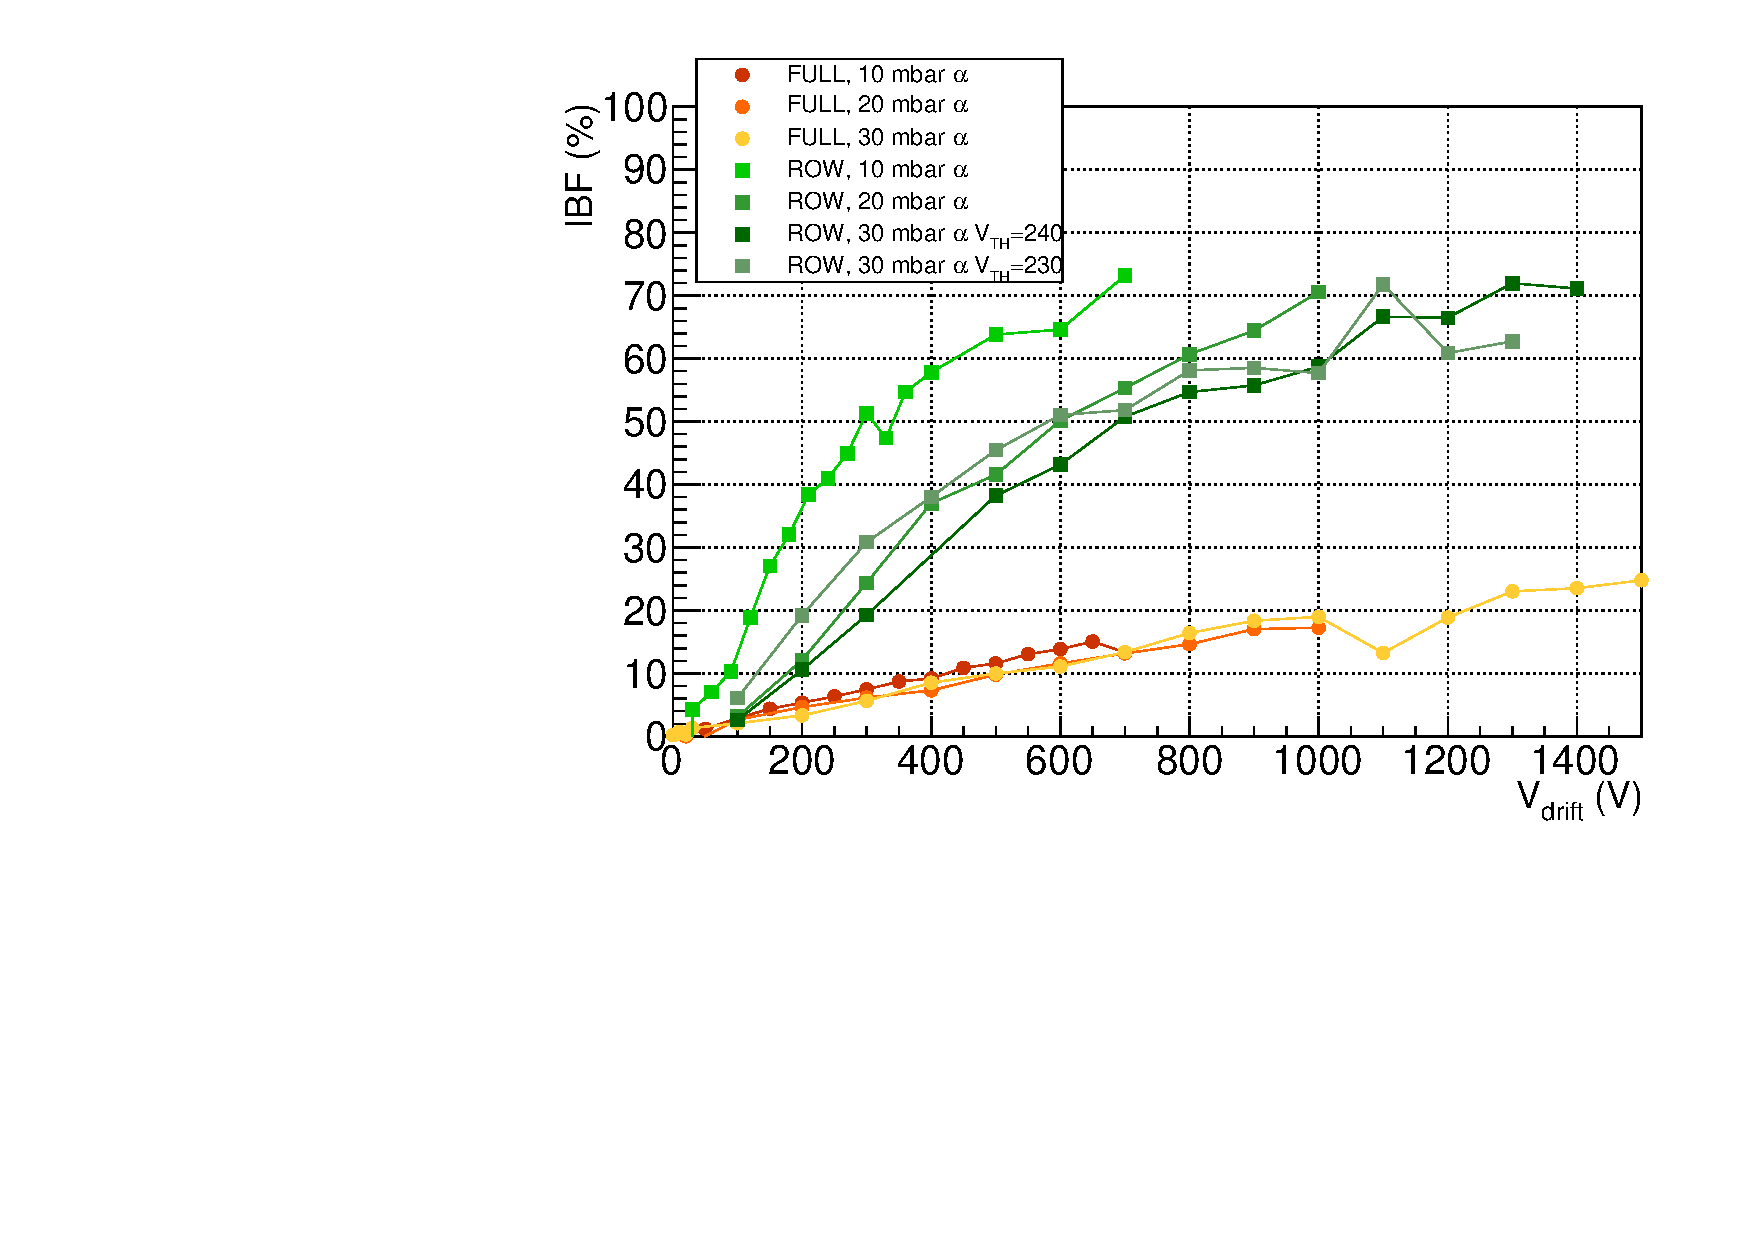
\includegraphics[width=0.9\textwidth]{Immagini/IBF_ALL_Comparison_nobeam.pdf}
	\caption{Comparison between the ion backflows evaluated for the ROW THGEM (square) and those 
	for the FULL THGEM (circle) as a function of \Vdrift{} for different pressure.}
	\label{fig:ion_backflow_FULLandROW}
\end{figure}

\begin{figure}[htbp]
	\centering
	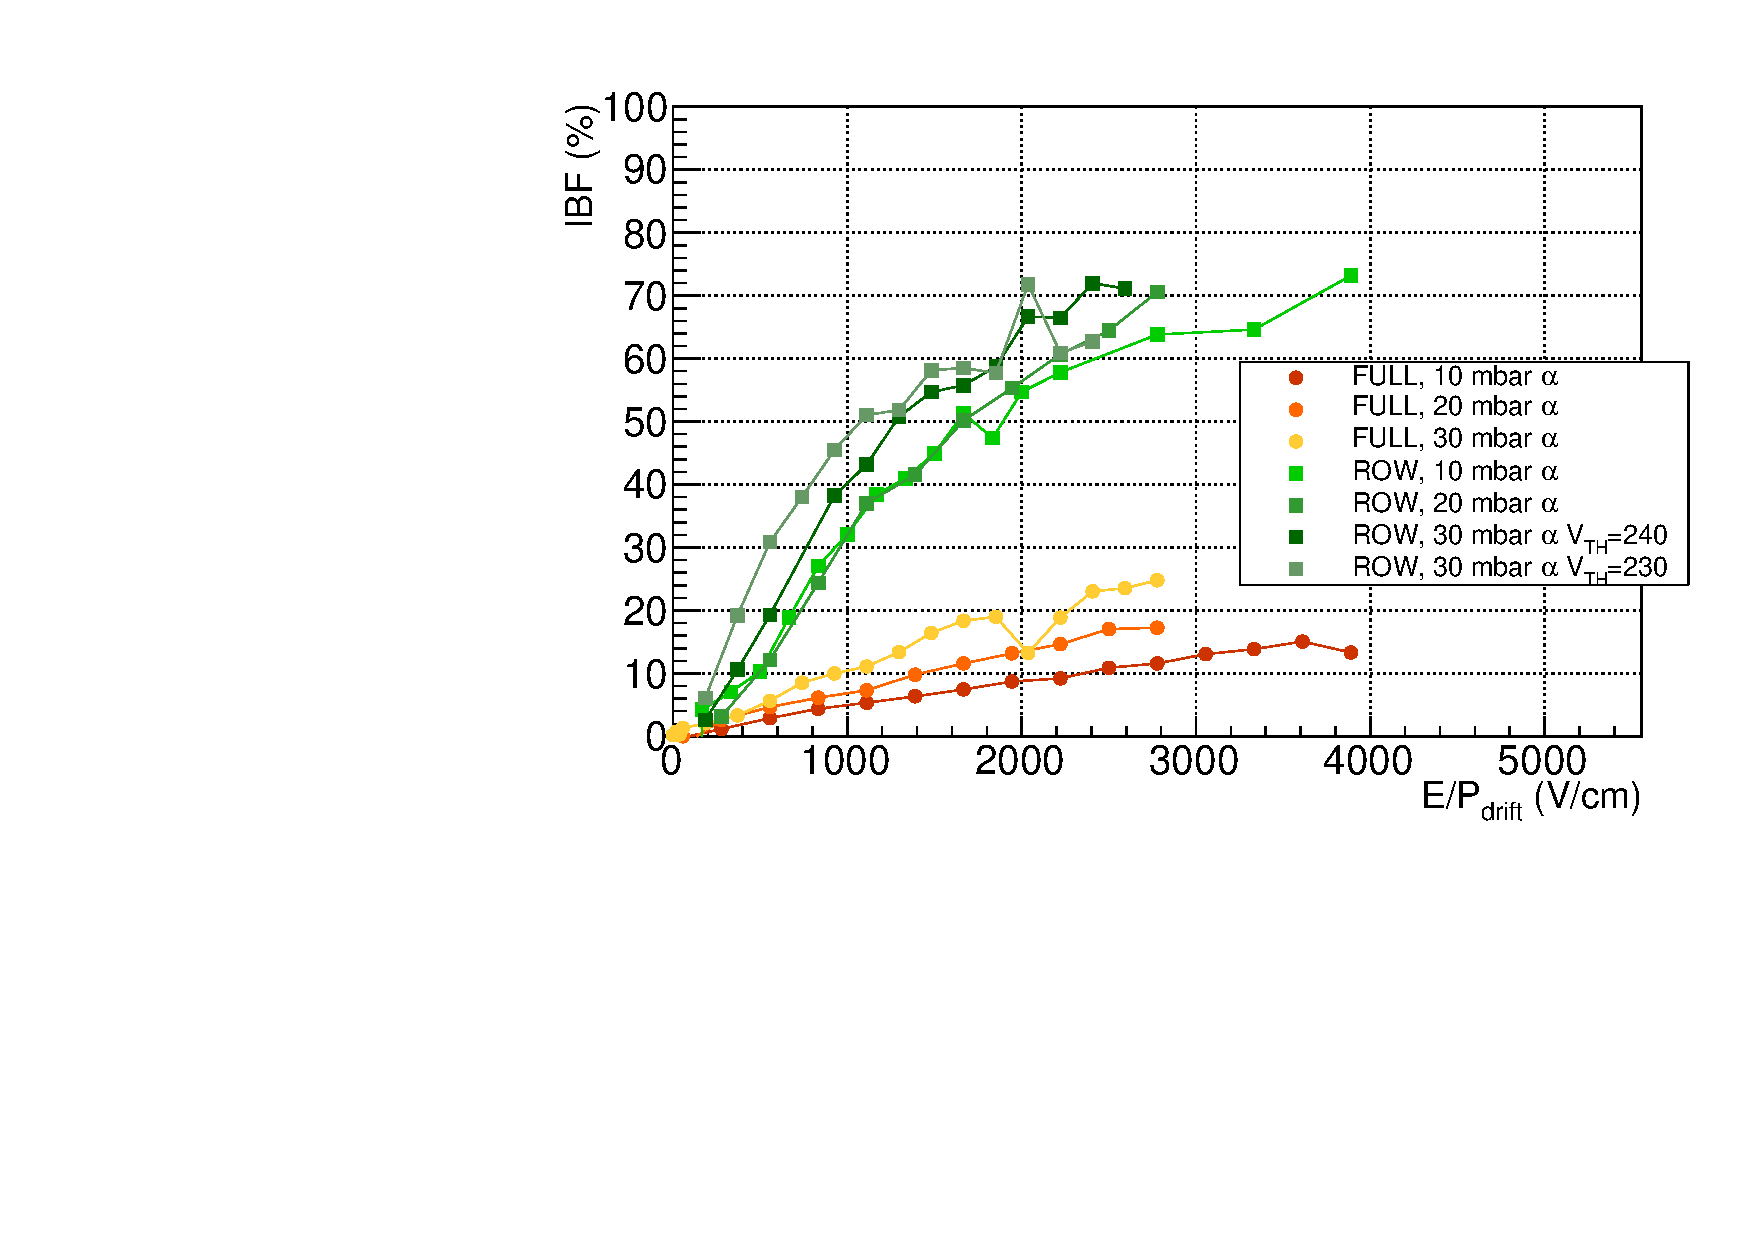
\includegraphics[width=0.9\textwidth]{Immagini/IBF_ALL_Comparison_nobeam_F.pdf}
	\caption{Comparison between the ion backflows evaluated for the ROW THGEM (square) and those 
	for the FULL THGEM (circle) as a function of the reduced electric field for different pressure.}
	\label{fig:ion_backflow_FULLandROW}
\end{figure}

\clearpage


%\subsubsection{Scan on \Vthgem}
%
%The new scan on \Vthgem{} was conducted fixing P~=~9.3~mbar, \Vind{} = 50 V and \Vdrift{} = 400 V.
%The measured currents have the same behaviour of the previous tests. Comparing this scan with a 
%previous one done in similar conditions (P~=~11~mbar, \Vind{} = 70 V, \Vdrift{} = 600 V), which is 
%shown in Figure~\ref{fig:thgem_FULLTHGEM_10mbar}, the relative distance between the anodic and the 
%top3 current is smaller. This is due to the different values of \Vind{}, that change the fraction 
%of electrons that can reach the anode respect to the number of electrons produced in total.
%\begin{figure}[p]
%	\centering
%	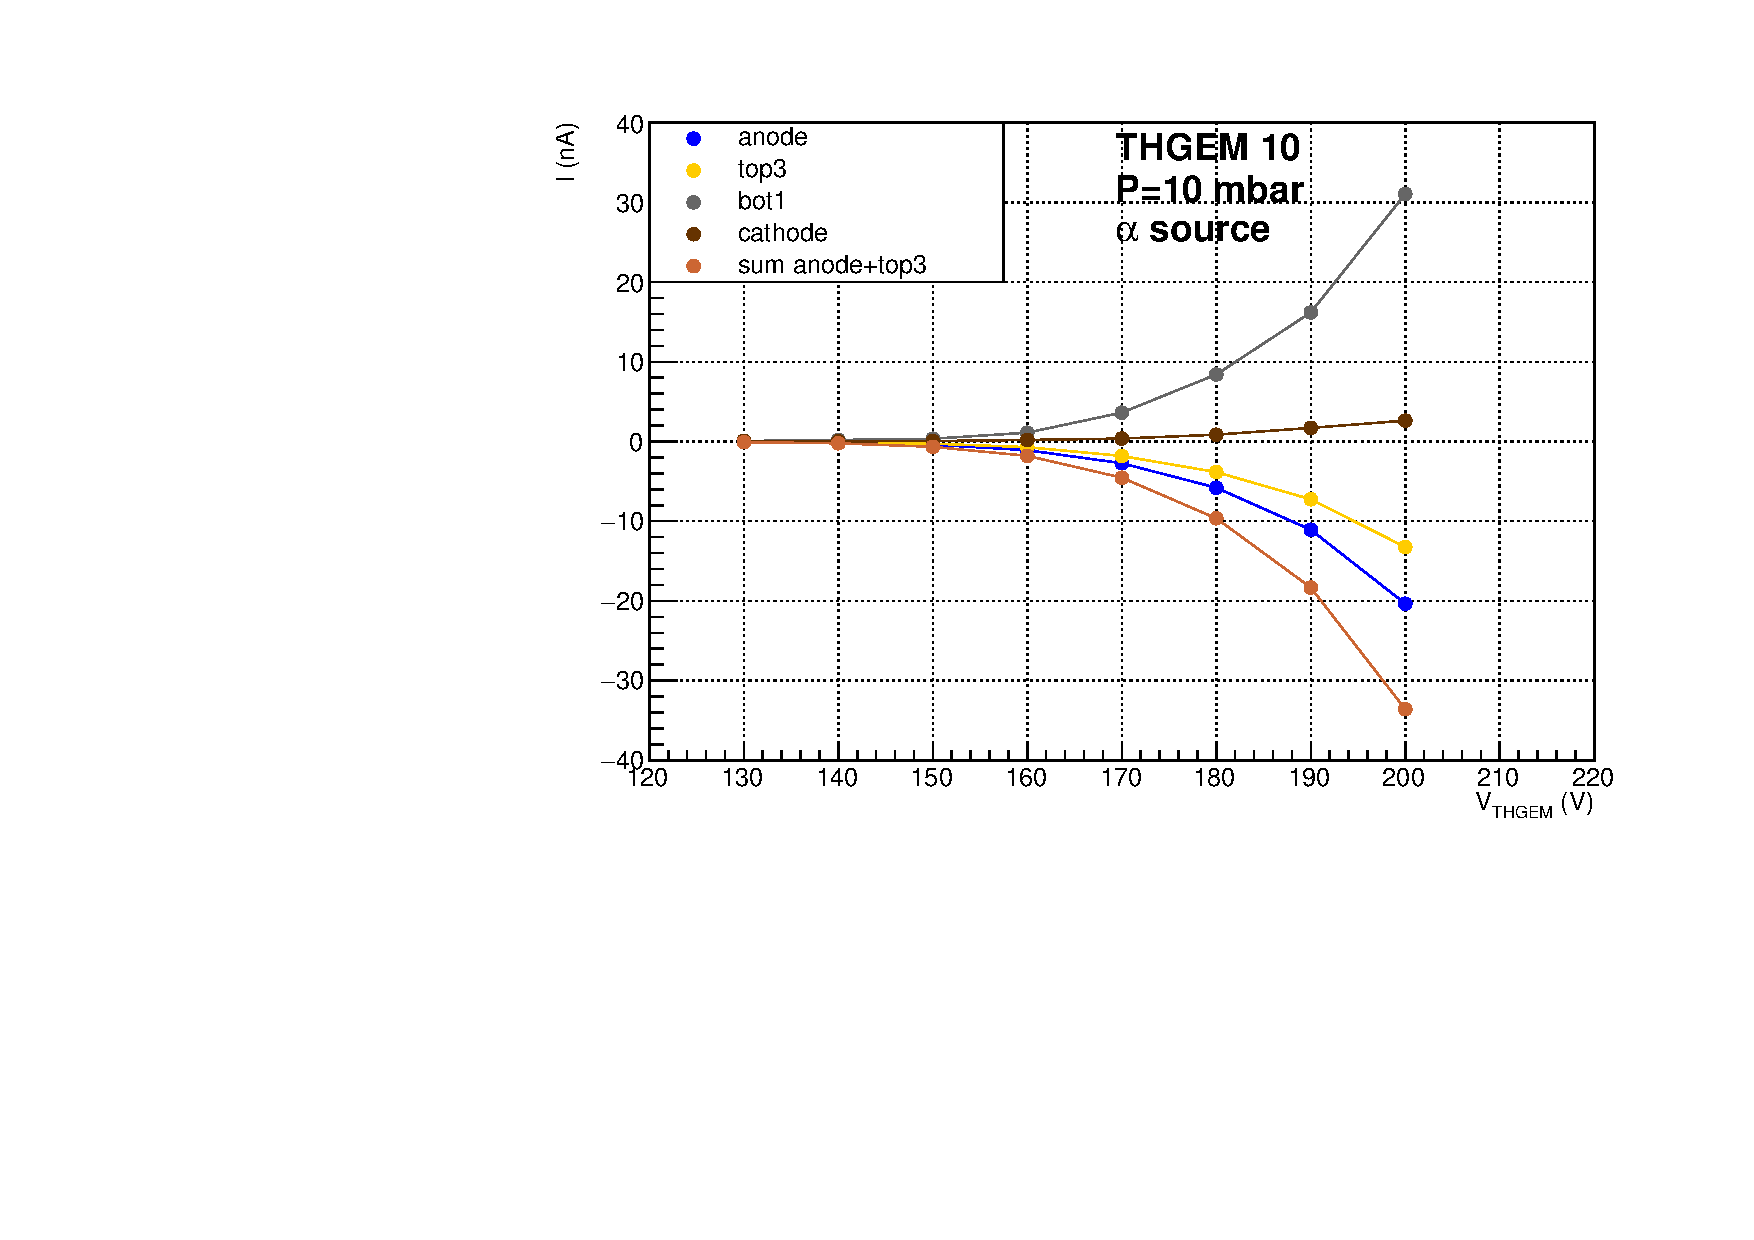
\includegraphics[width=\textwidth]{Immagini/thgemScan_THGEM10_10mbar_bis.pdf}
%	\caption{Currents measured during the scan on the voltage \Vthgem{} across each FULL THGEM at
%	 9.3~mbar, fixing \Vind~=~50~V and \Vdrift~=~400~V.}
%	\label{fig:thgem_FULLTHGEM_10mbar_bis}
%\end{figure}
%
%In Figure~\ref{fig:multiplication_factor_FULL_bis} is shown the multiplication factor (MF) 
%evaluated for this scan, in comparison with those previously calculated. The MF behaviour is 
%comparable to the measurement done in similar conditions. 
%
%\begin{figure}[!t]
%	\centering
%	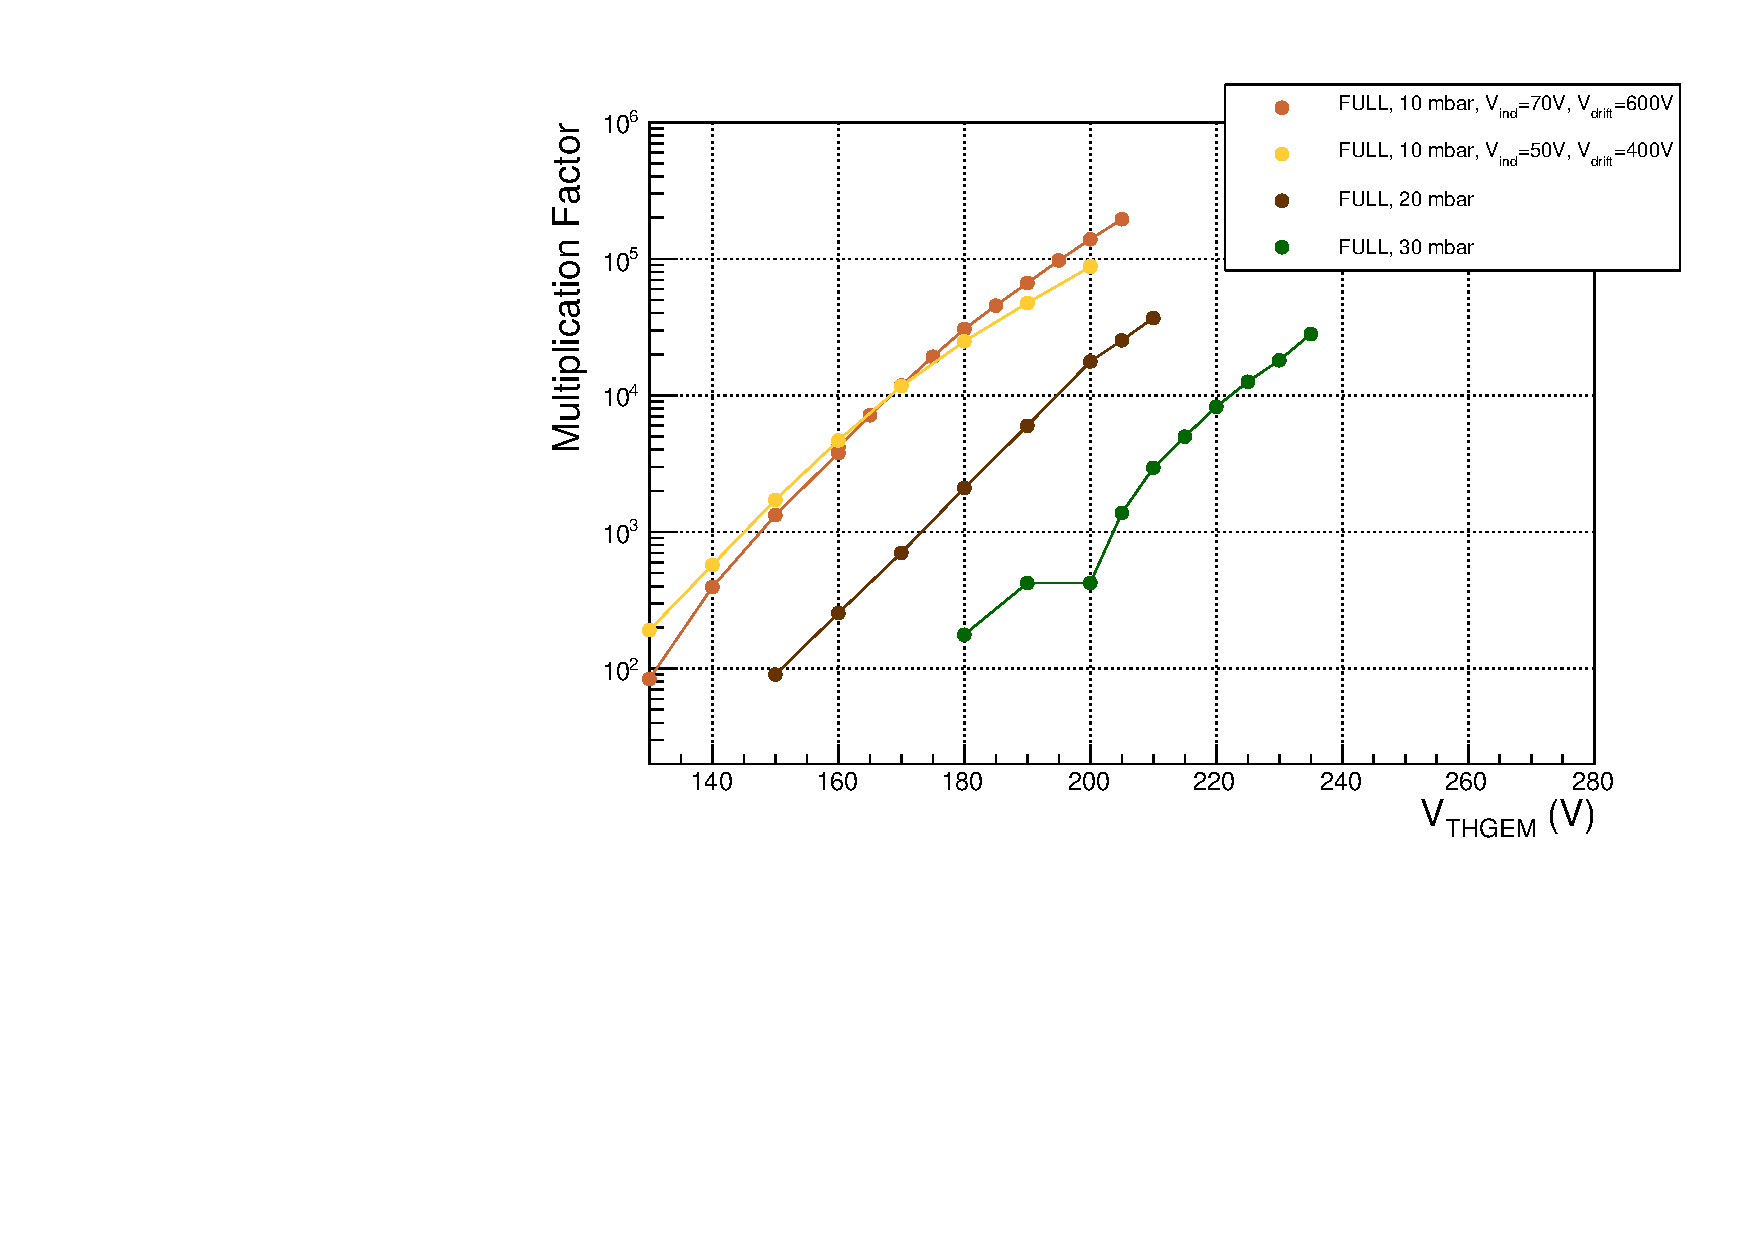
\includegraphics[width=\textwidth]{Immagini/MFvsTHGEM_FULL_bis.pdf}
%	\caption{The multiplication factors evaluated for the FULL THGEM as a function of \Vthgem{} 
%	and pressure.}
%	\label{fig:multiplication_factor_FULL_bis}
%\end{figure}
%\clearpage


%\begin{figure}[htbp]
%	\centering
%    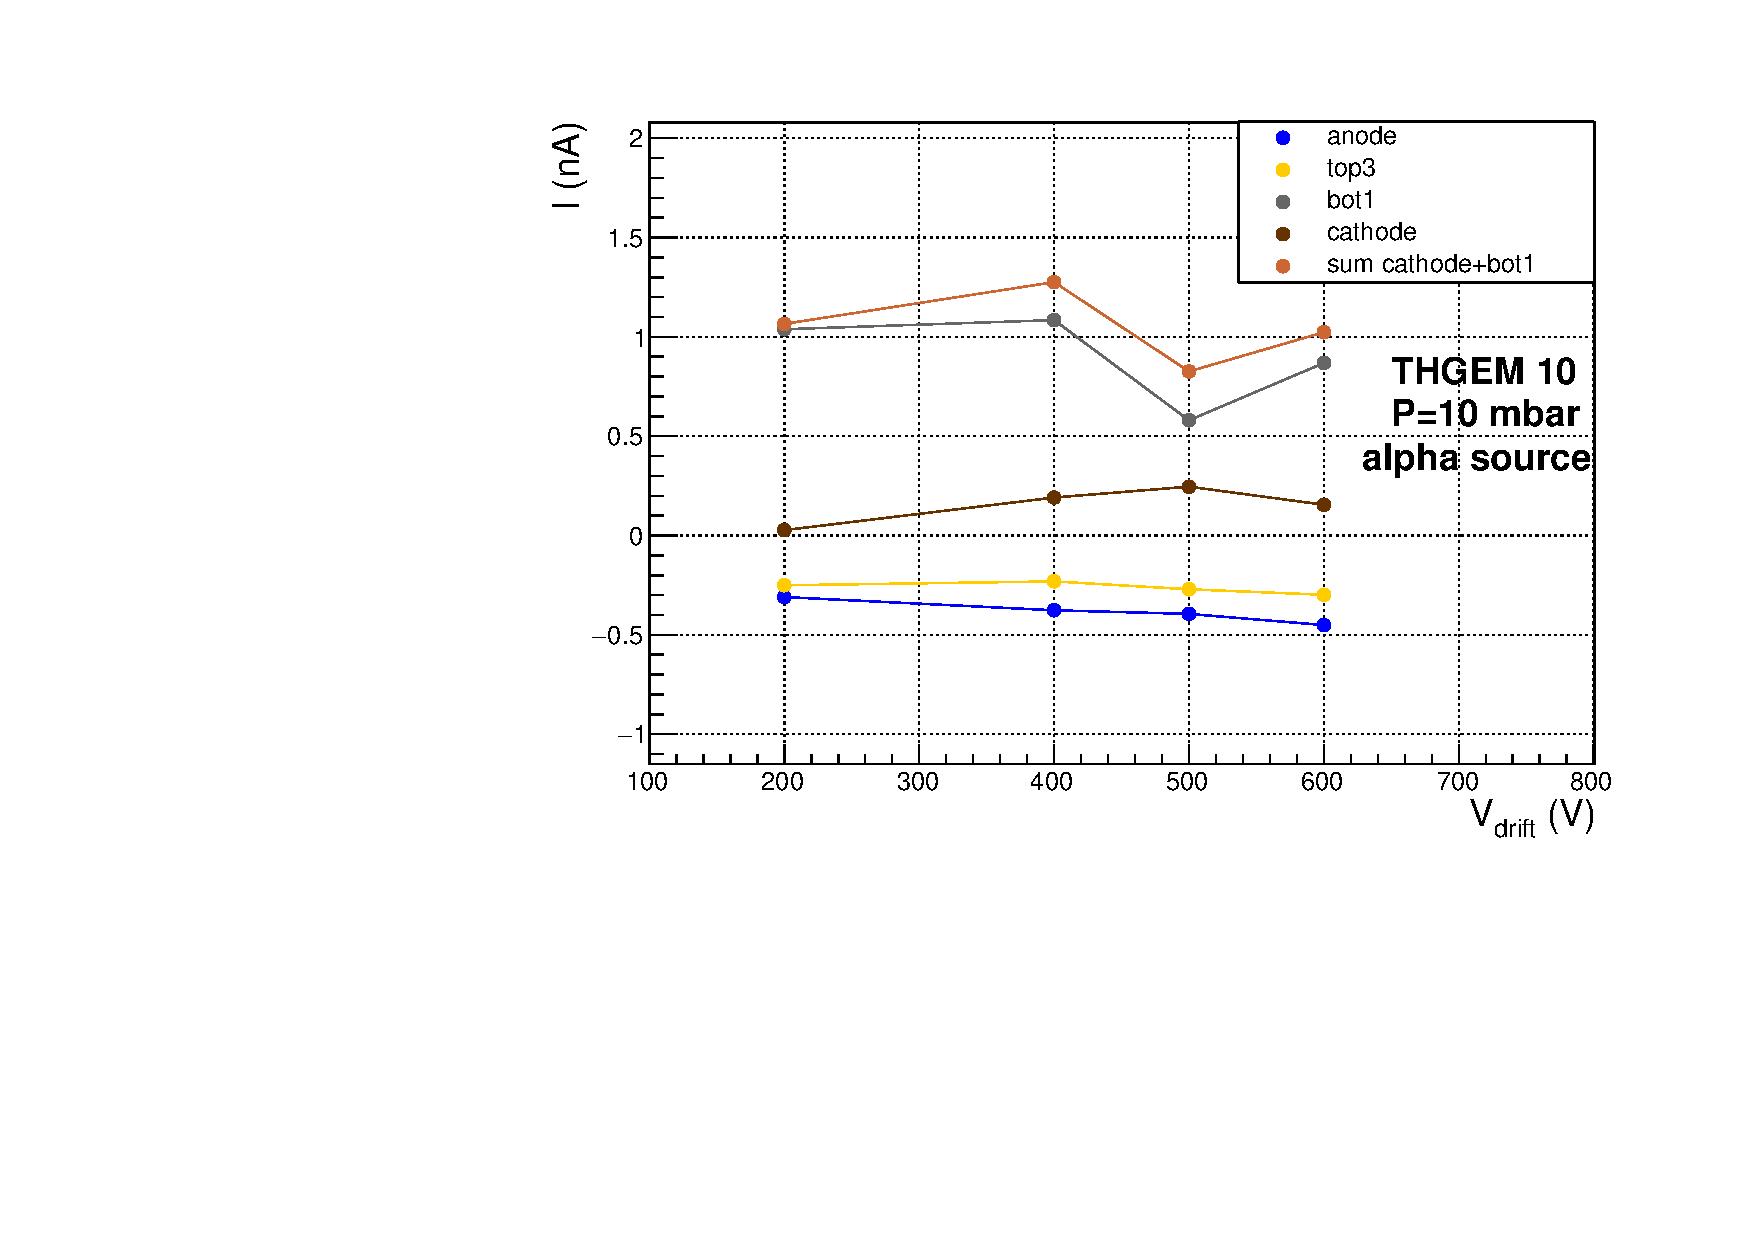
\includegraphics[width=\textwidth]{Immagini/driftScan_THGEM10_alpha_10mbar.pdf}
%	\caption{Currents measured during the scan on the voltage \Vdrift{} across the drift region at 
%	10~mbar.}
%	\label{fig:driftScan_THGEM10_alpha_10mbar}
%\end{figure}

\clearpage


%\section{First test with beam} \label{sec:test_beam}
%
%A first test with beam was performed on 19/02/2020. 
%
%A beam of $^{18}$O at an energy of 16.5 AMeV have been sent on a target of $^{116}$Cd xxx $\mu$
%The reaction products enter the scattering chamber housing the prototype that is located at an 
%angle of 30$^{\circ}$ respect to the beam direction. The pressure of isobutane inside the gas
% chamber was 9.4 mbar.
%Since at this energy the elastic cross section for the tracker prototype is not Rutherford It is 
%not possible to know the number and the kind of particles entering the prototype. The only 
%information on the flux comes from the faraday cup FC4 that is placed along the TeBe beam line 
%before the beam line gate valve. Therefore we have relative just relative information
%that allows to compare run with different beam currents but is not possible to extract
%absolute information on the particle rate entering the prototype, or make a comparison with
%$\alpha$ run.\\
%One possible way to compare such results with the alpha's is to compare directly the 
%anodic current even if it is not fully correct.
%Being equal all the parameters of the tracker (that is: P, \Vthgem{}, \Vind{}, \Vdrift{}),
%it should manifest the same behaviour if the total charge produced is the same, even if the 
%rate of particles entering the tracker is different.
%In fact even if the same current on the anode can be generate by a very different rates 
%of particles or heavy ions\footnote{Ion with different Z, M and energies loose quite different
%amount of energy\ldots} the effects on the tracker are mainly linked to the total amount of 
%charge produced and not on the rate of the particle\footnote{This is just partially thru. In fact 
%this is valid because we are measuring currents, it is no more if we study the signal on the 
%single strip of the anode. Moreover it is no strictly thru because there is a difference if
%the total primary charge is produced at very low rate with event that generate a lot of charge
%ore if the same total charge is produced at very high rate in events where a very small amount of 
%charge is produced}.
%
%Firstly the tracker was tested  at two values of the beam current 60 pA and 400 pA.
%In order to increase the beam current a collimator was remove from the beam line. In this way 
%we reached much higher values of the beam current: 1, 1.8 nA. Anyway since the 
%optic of the beam is not the same, that is the beam could reach the target with a different 
%emittance, is not correct to compare the first two beam currents
%with the second two\footnote{For example if the emittance of the beam was the same we can
%assert that with a beam of 1 nA we had a rate on the tracker that i s 2.5 times ahigher,
%since the emittance is not the same is not correct to affirm this, moreover also 
%the energy and Z of the particle reaching the tracker could be different.}
%
%An important difference respect to the case of the $\alpha$-source test is that the rate
%of the $\alpha$ particles is constant with a good approximation, the rate of the
%particle reaching the tracker in the in-beam test is not constant but fluctuate
%as the beam intensity.
%The fluctuation occur during the measurements of the currents, that is during the 1-2 minutes
%during which we take the average of the current and among one measurements and the others.
%Therefore the plot with beam are less precise and suffers the effect of the fluctuation.
%Unfortunately such uncertainty are not easy to extimate.
%
%
%\subsection{Scan on \Vthgem}
%The measurement was done at \Vind{} = 50~V and \Vdrift{} = 400~V with I$_{beam}$ 60 and 400 pA. 
%The plots of the currents vs \Vthgem are shown in Figure~\ref{fig:thgemScan_THGEM10_beam_10mbar}.
%The plots show have the same behaviour of the scan on \Vthgem{} with $\alpha$ source (see Figure~\ref{fig:thgem_FULLTHGEM_10mbar_bis}). 
%
%The discharge occurred at \Vthgem{} = 190 V with both beam intensities, to be compared with 
%\Vthgem{} = 210~V for the $\alpha$ case. 
%\begin{figure}[!htb]
%	\centering
%	\subfigure[]{ \label{fig:thgemScan_THGEM10_60pA_10mbar} 
%	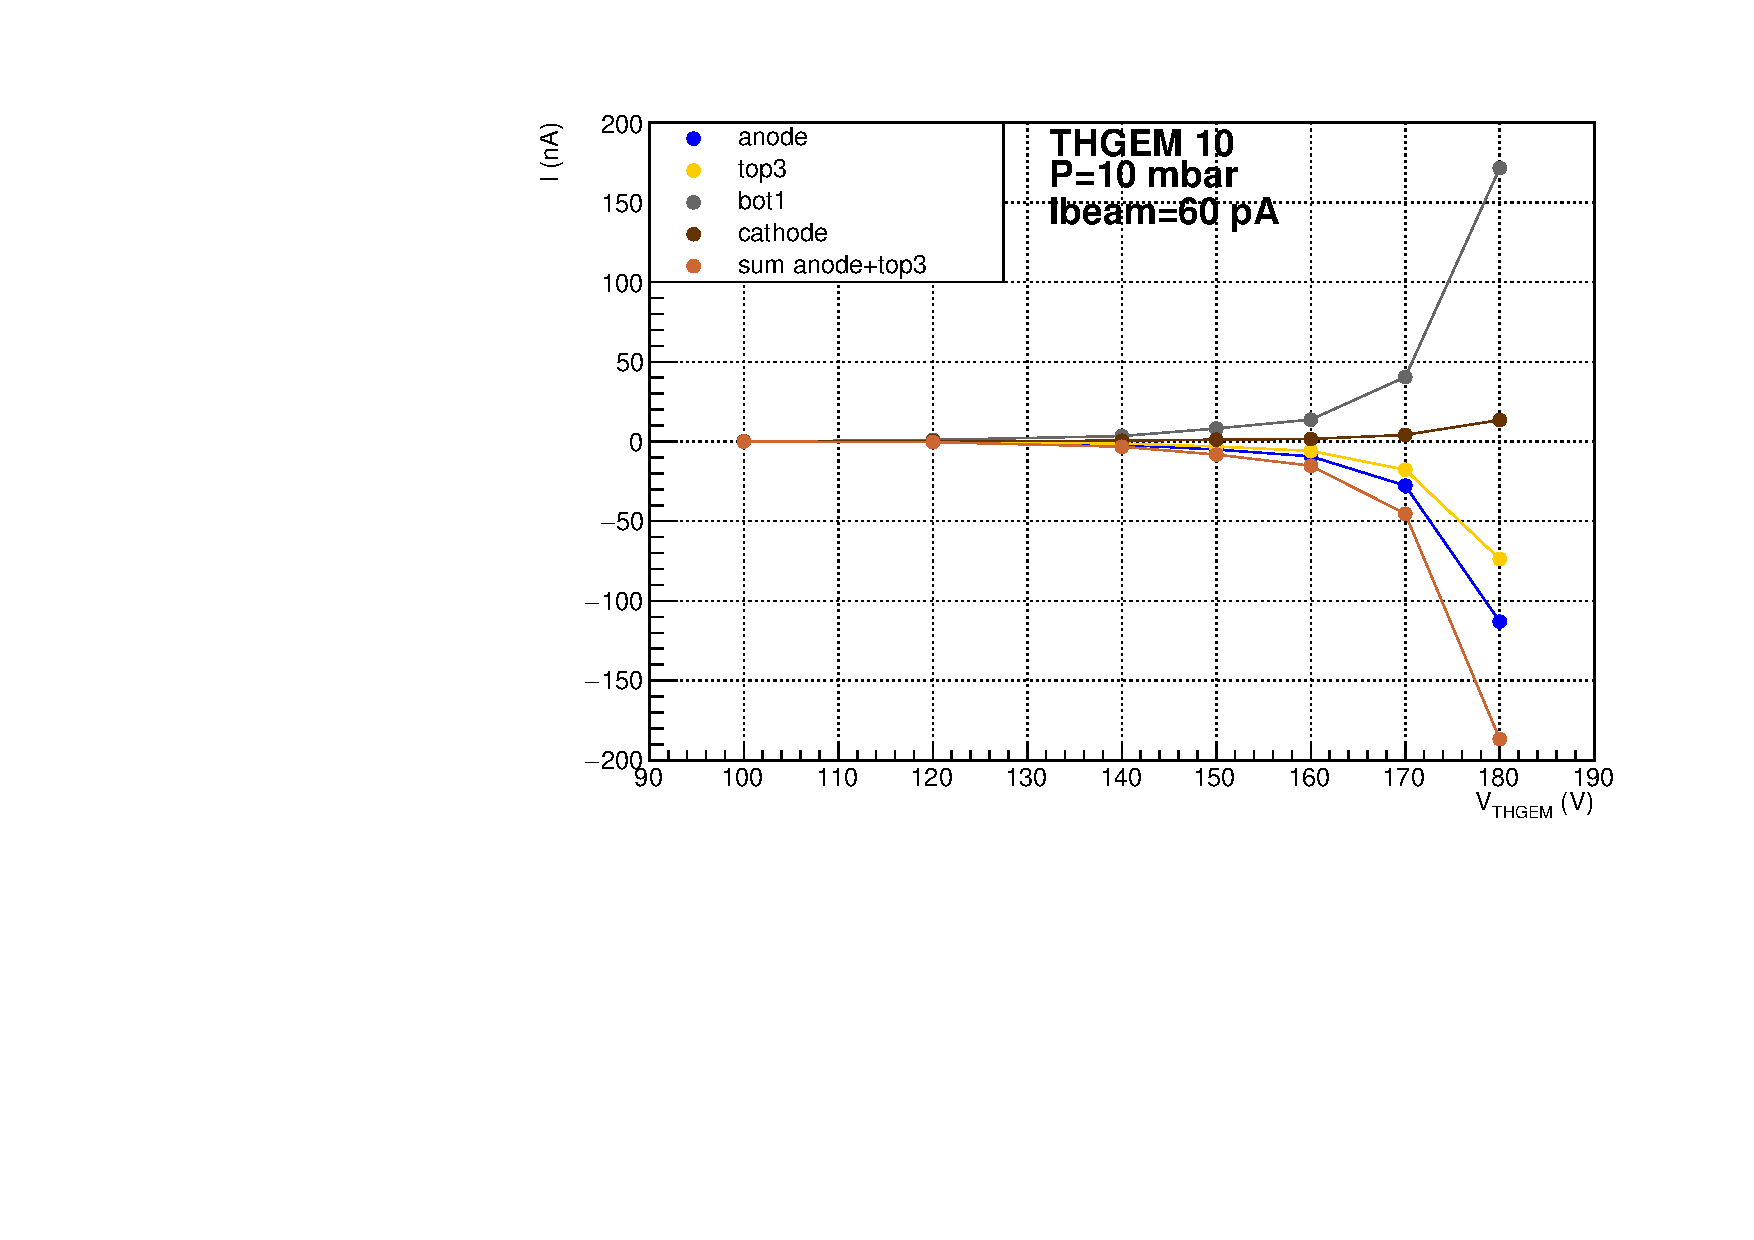
\includegraphics[width=0.96\textwidth]{Immagini/thgemScan_THGEM10_60pA_10mbar.pdf}}
%	\subfigure[]{ 	\label{fig:thgemScan_THGEM10_400pA_10mbar} 
%	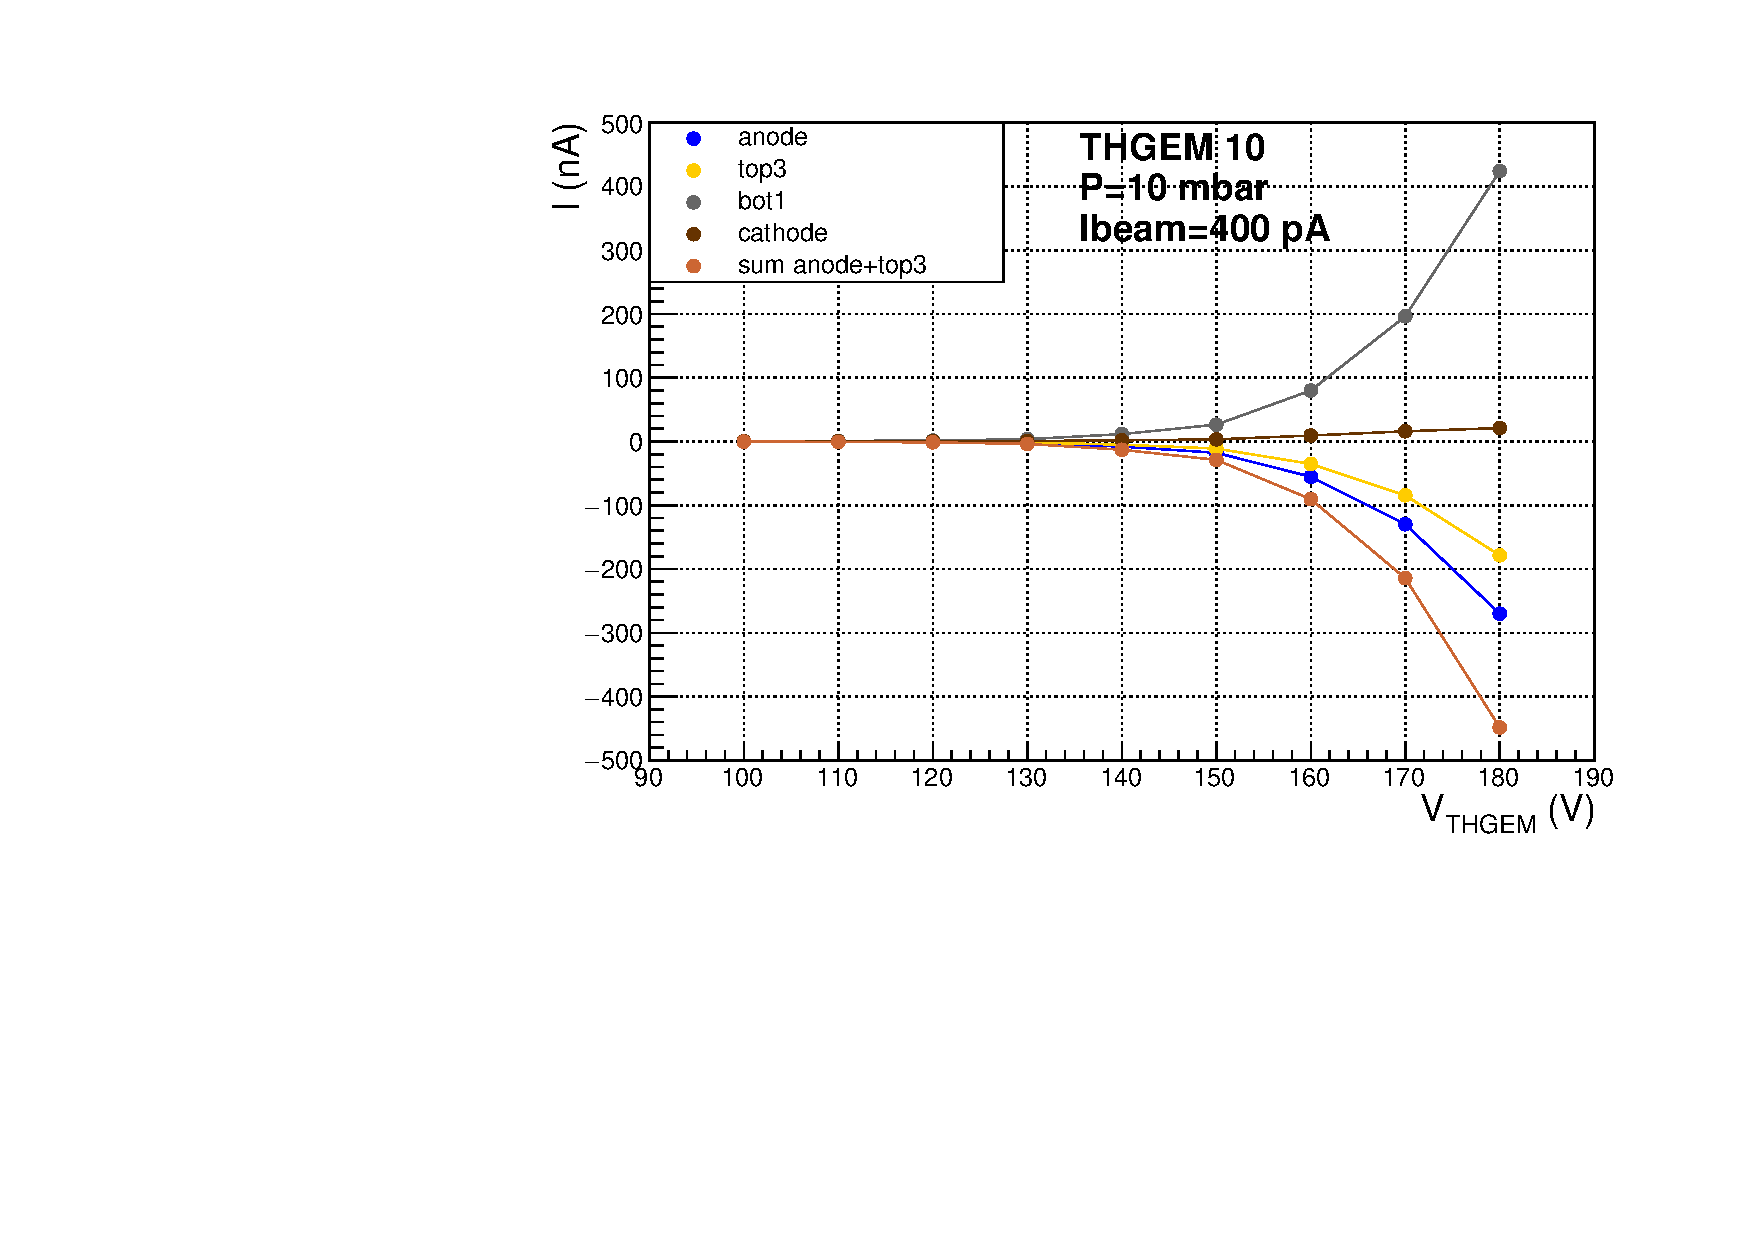
\includegraphics[width=0.96\textwidth]{Immagini/thgemScan_THGEM10_400pA_10mbar.pdf}}
%	\caption{Currents measured during the scan on the voltage \Vthgem{} across each FULL THGEM fixing 
%	\Vind{} = 50 V and \Vdrift{} = 400 V: in (a) at 60 pA, in (b) at 400 pA.}
%	\label{fig:thgemScan_THGEM10_beam_10mbar}
%\end{figure}
%\clearpage
%
%\subsection{Scan on \Vdrift}
%
%The measurement was done fixing \Vind{} = 50~V and \Vthgem{} = 160~V. 
%The plots of the currents vs \Vthgem are shown in Figure~\ref{fig:driftScan_THGEM10_beam_10mbar}.
%The currents have the same behaviour of the scan on \Vdrift{} with $\alpha$ source (see Figure~\ref{fig:driftScan_THGEM10_alpha_10mbar}). 
%The discharge voltage was 800 V with both beam intensities to be compared with about 750~V for the $\alpha$ source. Therefore, apparently there is no difference on the discharge voltage between the two cases
%$\alpha$-spurce, beam.
%%Another important difference is the maximum anodic achievable current: $\sim - $0.5 nA with $\alpha$ source, $\sim - $20~nA with \ibeam = 60~pA and $\sim - $55~nA with \ibeam = 400 pA.
%
%\begin{figure}[!htb]
%	\centering
%	\subfigure[]{ \label{fig:driftScan_THGEM10_60pA_10mbar} 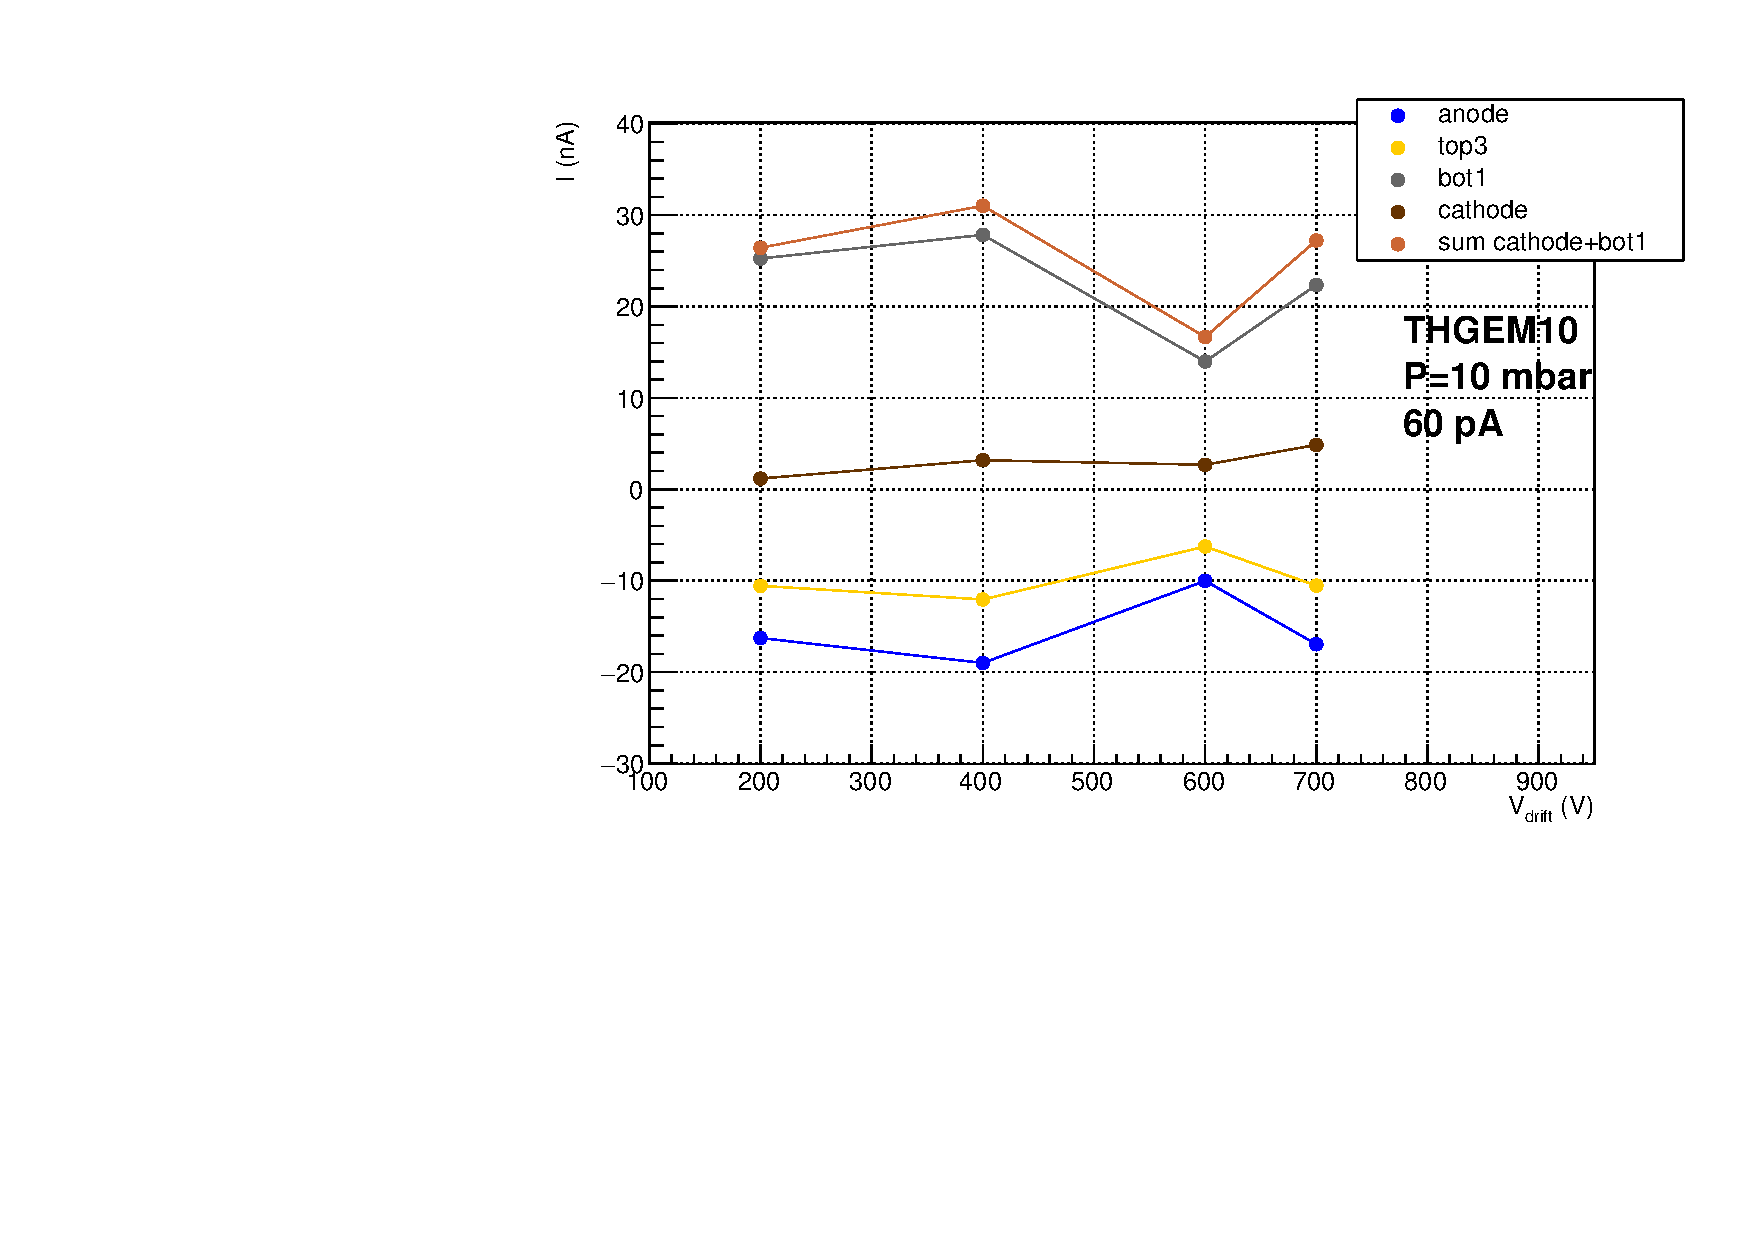
\includegraphics[width=0.96\textwidth]{Immagini/driftScan_THGEM10_60pA_10mbar.pdf}}
%	\subfigure[]{ 	\label{fig:driftScan_THGEM10_400pA_10mbar} 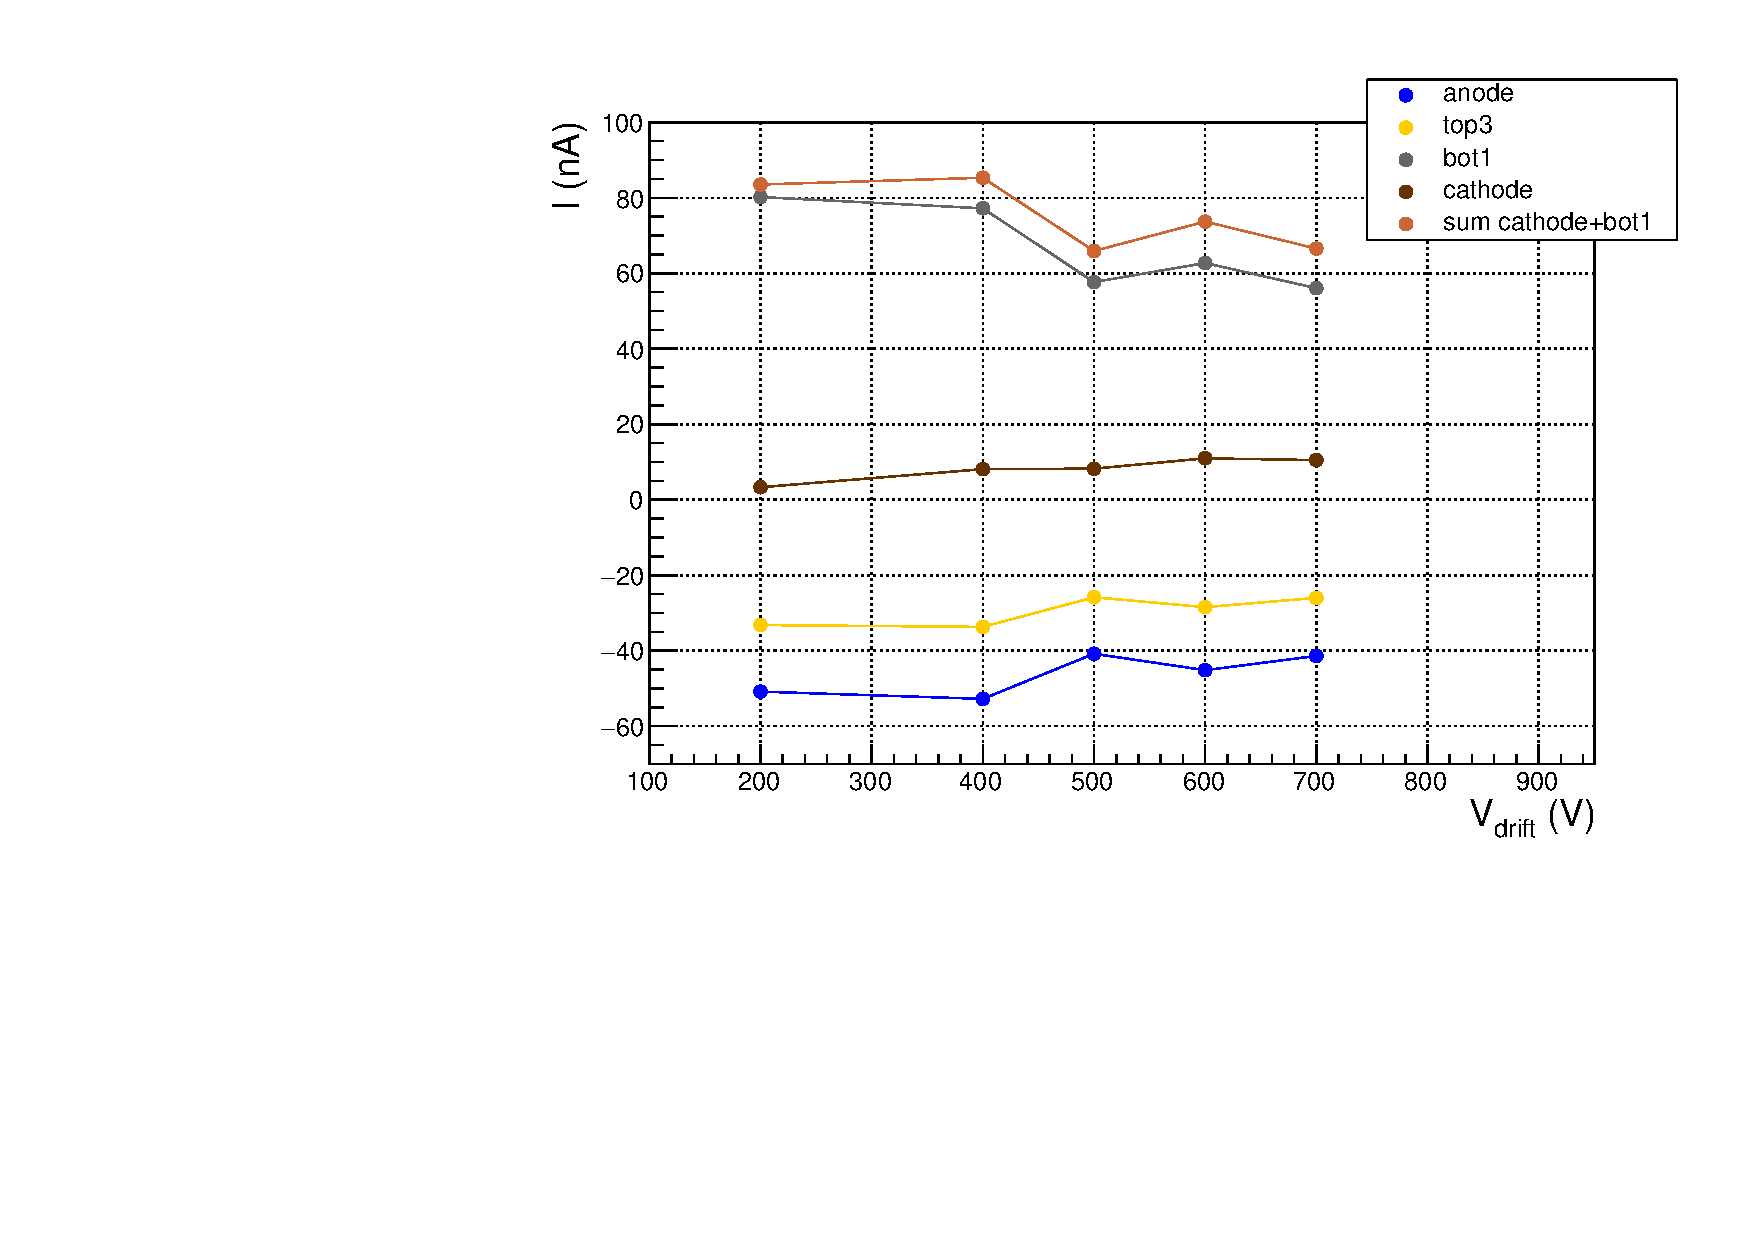
\includegraphics[width=0.96\textwidth]{Immagini/driftScan_THGEM10_400pA_10mbar.pdf}}
%	\caption{Currents measured during the scan on the voltage \Vdrift{} across each FULL THGEM fixing \Vind{} = 50 V and \Vthgem{} = 160 V: in (a) at 60 pA, in (b) at 400 pA.}
%	\label{fig:driftScan_THGEM10_beam_10mbar}
%\end{figure}
%
%
%%\clearpage
%
%\subsection{Ion Backflow  (IBF)}
%Figure~\ref{fig:IBFvsDrift_withBeam} shows the IBF calculations as a function of \Vdrift{} for \ibeam{} equal to 60 and 400~pA. 
%Comparing the two curves we can affirm that there are no significant differences of the
%IBF for the two beam currents. 
%
%\begin{figure}[htbp]
%	\centering
%	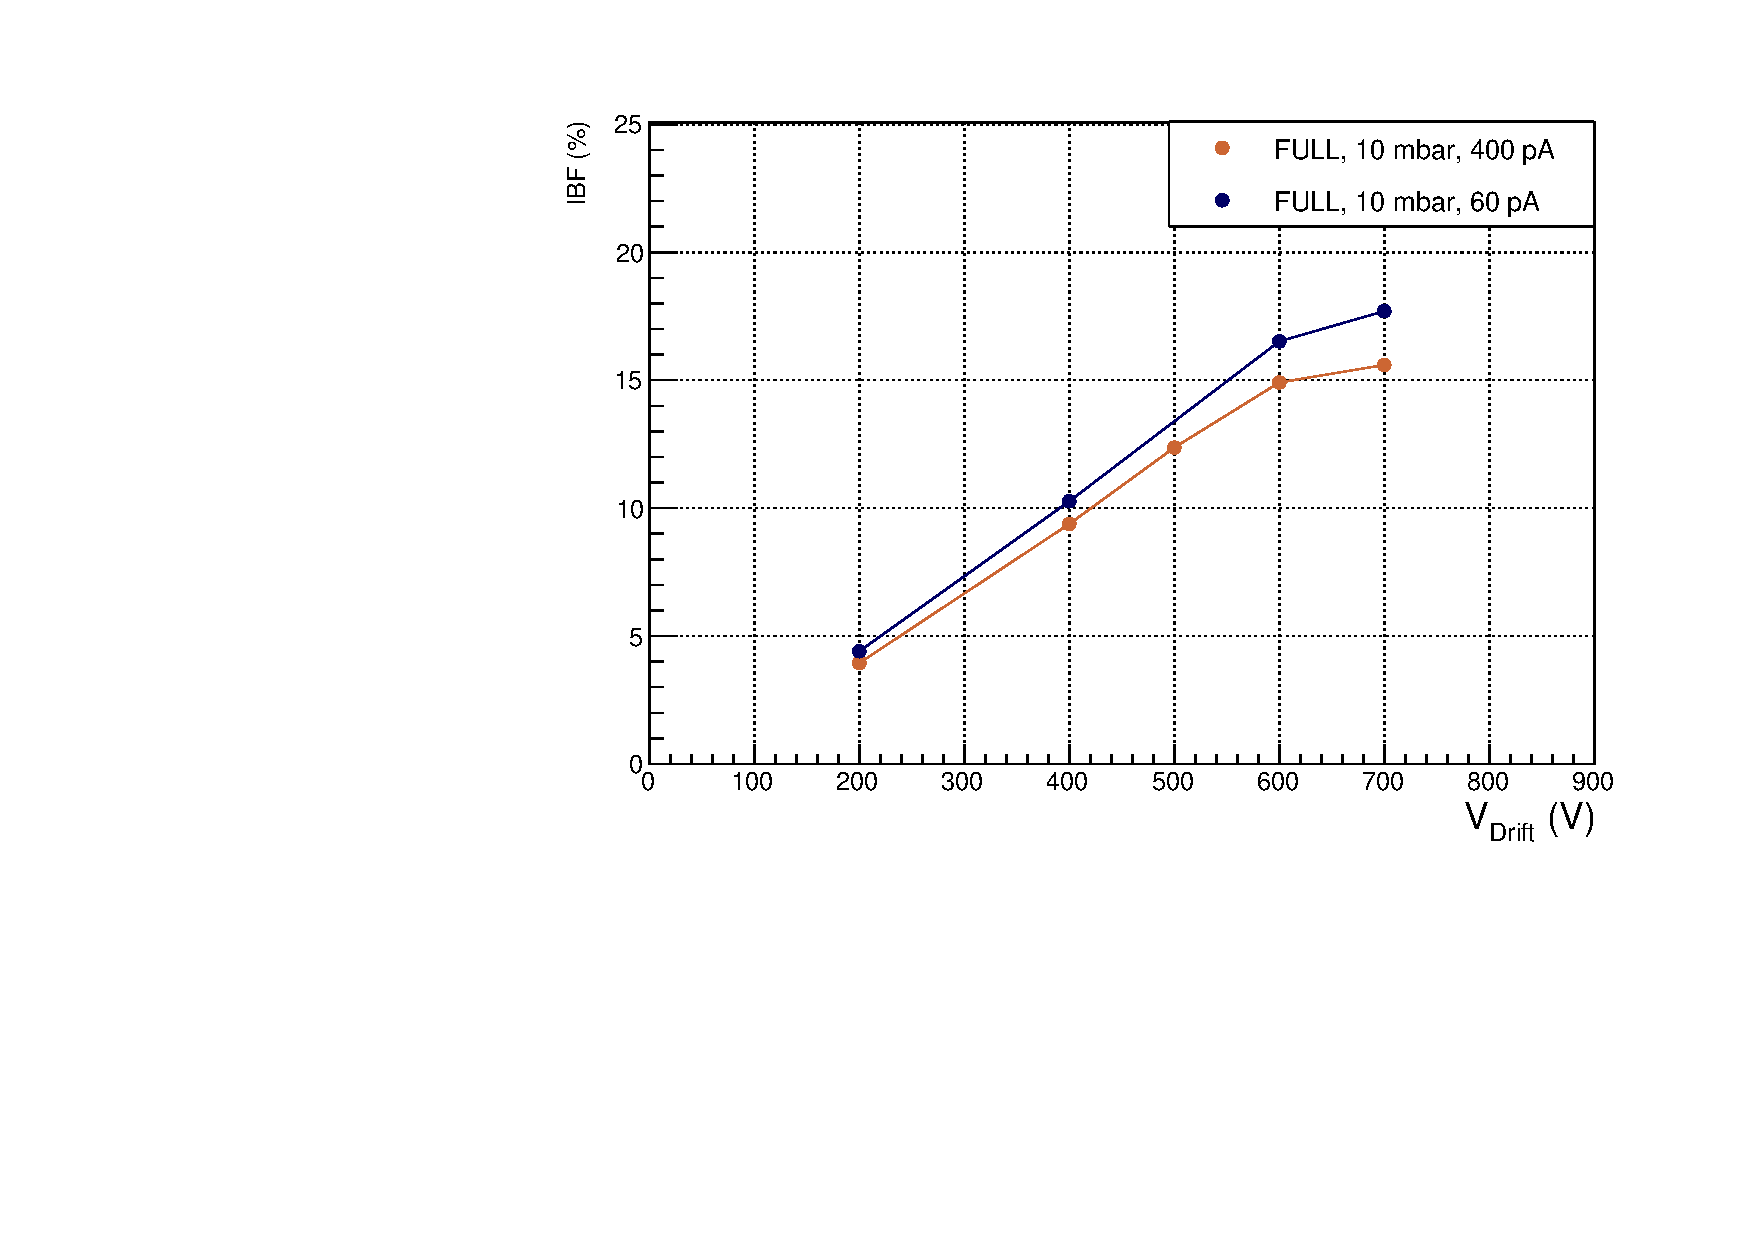
\includegraphics[width=\textwidth]{Immagini/IBFvsDrift_withBeam.pdf}
%	\caption{Ion backflow evaluated for FULL THGEM as a function of \Vdrift{} at 60 pA and 400 pA fixing \Vind{} = 50 V and \Vthgem{} = 160 V.}
%	\label{fig:IBFvsDrift_withBeam}
%\end{figure}
%
%%In Figure~\ref{fig:IBFvsDrift_beam_alpha_average}, IBF was studied as a function of \Vdrift{}. 
%Figure~\ref{fig:IBFvsDrift_beam_alpha_average} shows a comparison between the IBFs with $\alpha$ 
%source and those with beam. 
%%The IBF for 60 pA, 400 pA at \Vthgem{} = 160 V and $\alpha$ source  at \Vthgem{} = 190 V has a maximum IBF of 17\%. 
%%In the test with $\alpha$ source, when \Vthgem{} is less than 190 V the cathode current is so small 
%%that IBF estimate is not reliable. 
%IBF as a function of \Vdrift{} seems not sensible to the rate because the curves are basically the same
%for beam and alpha-source.
%%This is not well understood.
%There are also few points taken at different value of beam currents but at a single value of \Vdrift.
%The trnd seems that increasing the beam current and fixing all the other parameters, the IBF decreases. 
%This effect anyway is not so clear and could be simply due to the large uncertainties of the 
%measurements.
%
%\begin{figure}[htbp]
%	\centering
%	\includegraphics[width=\textwidth]{Immagini/IBFvsDrift_beam_alpha_average.pdf}
%	\caption{Ion backflow evaluated for FULL THGEM as a function of \Vdrift{} at 60 pA, 400 pA, 1 nA, 1.8 nA and with $\alpha$ source.}
%	\label{fig:IBFvsDrift_beam_alpha_average}
%\end{figure}
%
%IBF was studied also as a function of \Vthgem: the results are shown in 
%Figure~\ref{fig:IBFvsTHGEM_beam_alpha}. IBF is nearly constant with varying \Vthgem. The best 
%condition to have IBF as less as possible is to work near \Vthgem{} = 200 V but as far as possible 
%from discharge.\\
%
%\begin{figure}[!p]
%	\centering
%    \includegraphics[width=1.\textwidth]{Immagini/IBFvsTHGEM_beam_alpha_zoom.pdf}
%	\caption{Ion backflow evaluated for FULL THGEM as a function of \Vthgem{} at 60 pA, 400 pA, 1 nA, 
%	1.8 and with $\alpha$ source.}
%	\label{fig:IBFvsTHGEM_beam_alpha}
%\end{figure}
%
%IBF was studied also as a function of \Vind: the results are shown in Figure~\ref{fig:IBFvsInd_beam}. 
%As already said, IBF for ROW THGEM is much bigger than that for FULL THGEM. Another difference is 
%that IBF is constant for FULL THGEM and it decreases for ROW THGEM. IBF is not dependent on 
%pressure and it maybe decreases with increasing beam current.
%
%\begin{figure}[!t]
%	\centering
%	\includegraphics[width=\textwidth]{Immagini/IBFvsInd_beam.pdf}
%	\caption{Ion backflow evaluated for FULL THGEM as a function of \Vind{} at 60 pA, 400 pA, 1 nA, 
%	1.8 nA and with $\alpha$ source.}
%	\label{fig:IBFvsInd_beam}
%\end{figure}
%
%
%\subsection{Scan on the rate}
%
%\textcolor{red}{Ha senso mettere questa parte?}\\
%In Figure~\ref{fig:IbeamScan_THGEM10_10mbar_average} the measured currents were plotted as a function of the beam current (\ibeam). 
%%We expected a linear behaviour, but instead we found an exponential one. This behaviour can be explained because the point at 60 pA and 400 pA have different conditions from the others. 
%It is important to remember the discussion done at the beginnign of the section
%that is that the points at 1 and 1.8 nA where obtained with a beam that had
%a difference emittance respect to the point at 60 and 400 pA.
%Therefore the scaling of the rate from the first tow points to the second two is not correct.
%
%
%\begin{figure}[htbp]
%	\centering
%	\includegraphics[width=\textwidth]{Immagini/IbeamScan_THGEM10_10mbar_average.pdf}
%	\caption{Currents measured with varying \ibeam.}
%	\label{fig:IbeamScan_THGEM10_10mbar_average}
%\end{figure}

\clearpage
\section{Second test with beam} 

The test was performed in march 2020.
A beam of $^{18}$O at 145 MeV was sent on two gold targets 0.972 and 9.6 mg/cm$^2$ thick.
The beam intensity was measured by mean of two faraday cups: one upstream the target
(MXFC1) and a second downstram the target (TebeFC) that has a lower sensitivity.
The tracker prototype is located a 30$^{\circ}$ respect to the beam direction, at this energy 
the elastic scattering is Rutherford therefore it is possible to calculate the number of 
$^{18}$O particles entering the detector.
The solid angle\footnote{Distance from the target 470mm and area 108$\times$120 mm$^2$} of the 
prototype was about 6$\cdot$10$^{-2}$ sr while the angular range covered is 30$^{\circ} \pm$ 
6.6$^{\circ}$. Also a charged particle detector was placed downstream the 
prototype. It was a silicon photodiode 1$\times$1cm$^2$ covering a solid angle\footnote{Distance 
from the target 470+130mm} of 3$\cdot$10$^{-4}$, while the anglar range covered is 30$^{\circ} \pm$ 0.47$^{\circ}$.

The rate of particle entering the prototype was estimated when possible in two independent
ways: Assuming a Rutherford scattering, knowing target thickness and beam current\footnote{Since,
in same case the current read by TBFC2 was below the its sensitivity the faraday cup 
TBFC1 was used to estimate the current on the target after a scaling.}; 
scaling the counting rate in the photodiode to the solid angle of the tracker 
prototype\footnote{The scaling factor is 129.6=12*10.8.}.

The energy lost by $^{18}$O in 10 mbar of C$_4$H$_{10}$ is about one forth of those of the
$\alpha$ used in previous tests, i.e. 1 MeV to be compared with the 270keV lost by $\alpha$
at 5.485 MeV.


In Table \ref{tab:current_rate} a scheme of the currents and relative rates used in the test.

\begin{table} [!h]
	\begin{center}
		\renewcommand{\arraystretch}{1.2}
		\begin{tabular} {ccccccccccc}
			MXFC1   & & TeBeFC  & & $I_{beam}^{estim}$ & & Target thick.	& & $R_{calc}$ & & $R_{pd}$ \\
			(pA)  	& &   (pA)  & &       (pA)		   & &  (mg/$\mbox{cm}^2$)&&  (pps)   & &   (pps)   \\
			\toprule[0.1em]
			%\hline
			900	& & 400	& &	-		& & 9.6		& & 3400	& & 13.4		\\
			680	& &	280	& & -		& & 9.6		& &	2400	& & 8.8			\\
			220	& & 100	& & - 		& & 9.6		& & 850		& & 2.5			\\
			100	& & 60	& & - 		& & 9.6		& & 500 	& & 1.6			\\
			100	& & NR	& & 45 		& & 0.972	& & 40  	& & $\sim$0.2	\\
			250	& & NR	& & 110		& & 0.972	& & 90  	& & $\sim$0.3	\\
			680	& &	300	& & -		& & 0.972	& &	240		& & $\sim$1		\\
			250	& & 150	& & - 		& & 9.6		& & 1300	& & 3.4			\\
			250	& & 160	& & - 		& & 0.972	& & 130 	& & 0.3			\\
			\bottomrule[0.1em]
		\end{tabular}
	\end{center}
	\caption{The values of beam currents, measured by MXFC1 and TeBeFC; the beam current estimated ($I_{beam}^{estim}$) when TeBeFC was not able to read the current; the target thickness; the calculated rate ($R_{calc}$) of particles impinging on the tracker and the rate ($R_{pd}$) of particles measured by the photodiode detector.} \label{tab:current_rate}
\end{table}

\clearpage
%%%%%%%%%%%%%%%%%%%%%%%%%%%%%%%%%%%%%%%%%%%%%%%%%%%%%%%%%%%%%%%%%%%%%%%%%%%%%%%%%%%%%%%%%%%%%%%%%%%
%%%%%%%%%%%%%%%%%%%%%%%%%%%%%%%%%%%%%%%%%%%%%%%%%%%%%%%%%%%%%%%%%%%%%%%%%%%%%%%%%%%%%%%%%%%%%%%%%%%
\subsection{FULL THGEM}

  \subsubsection{THGEM scan}
  The two scans of the \Vthgem{} done at low rate 90 pps and high rate 3400 pps are shown in Fig.
  \ref{fig:driftScan_withBeam_H} and \ref{fig:driftScan_withBeam_L}.
  \begin{figure}[htbp]
	\centering
	\includegraphics[width=\textwidth]
	{Immagini/thgemScan_THGEM10_20mbar-Vdrift1000V-2020-03-09.pdf}
	\caption{\Vthgem{} scan for the highest beam intensity 3400 pps. }
	\label{fig:driftScan_withBeam_H}
  \end{figure}
  \begin{figure}[htbp]
	\centering
	\includegraphics[width=\textwidth]
	{Immagini/thgemScan_THGEM10_20mbar_109pA-Vdrift1000V-2020-03-09_logscale.pdf}
	\caption{\Vthgem{} scan for the lowest beam intensity 87pps.}
	\label{fig:driftScan_withBeam_L}
  \end{figure}
  In Fig. \ref{fig:MF_FULL_beam} a comparison of the multiplication factor as a function of the
  voltage \Vdrift{} for run with $\alpha$ source and beam is shown. 
  \begin{figure}[htbp]
	\centering
	\includegraphics[width=\textwidth]{Immagini/MF_FULL_THGEM_withBeam.pdf}
	\caption{MF for the FULL THGEM as a function of the \Vthgem{}. Run with $\alpha$-source
	and $^{18}$O beam are compared. }
	\label{fig:MF_FULL_beam}
  \end{figure}
  In Fig. \ref{fig:MF_FULL_beam_F} same data of Fig. \ref{fig:MF_FULL_beam} but plotted as a 
  function of the reduced electric field of the THEGEM. Some clarification on how the reduced 
  electric field was calculated is necessary. Obviously make no sense to speak about a value of 
  the electric field inside the THGEM since the electric field is not uniform there. We make a very
  strong approximation that is calculate the electric field as it was uniform that is V/d.
  \begin{figure}[htbp]
	\centering
	\includegraphics[width=\textwidth]{Immagini/MF_FULL_THGEM_withBeam_F.pdf}
	\caption{MF for the FULL THGEM as a function of the reduced electric field in the THGEM. Run 
	with $\alpha$-source and $^{18}$O beam are compared.}
	\label{fig:MF_FULL_beam_F}
  \end{figure}


  In Fig. \ref{fig:IBF_FULL_thegem_beam} A comparison of the IBF for FULL THGEM including
  run with $\alpha$-source and with beam.
  \begin{figure}[htbp]
	\centering
	\includegraphics[width=\textwidth]{Immagini/IBF_FULL_THGEM.pdf}
	\caption{ibf for FULL THGEM as a function of the \Vthgem{}. Run with $\alpha$-source
	and $^{18}$O beam are compared. }
	\label{fig:IBF_FULL_thegem_beam}
  \end{figure}
  
  \clearpage
%%%%%%%%%%%%%%%%%%%%%%%%%%%%%%%%%%%%%%%%%%%%%%%%%%%%%%%%%%%%%%%%%%%%%%%%%%%%%%%%%%%%%%%%%%%%%%%%%%%
 \subsubsection{Drift scan}

  In fig. \ref{fig:DriftScan_FULL_beam} the scan of the \Vdrift{} is shown. A difference respect
  to the $\alpha$ case is the fact that in the present case the anodic current is increasing up to
  about 600 V and after is constant, while with $\alpha$ the anodic current is almost
  constant at all the \Vdrift values.
  \begin{figure}[htbp]
	\centering
	\includegraphics[width=0.95\textwidth]{Immagini/driftScan_THGEM10_20mbar-Vthgem205V-2020-03-09.pdf}
	\caption{IBF for the FULL THGEM as a function of \Vdrift. Run with 
	$\alpha$-source	and $^{18}$O beam are compared.}
	\label{fig:DriftScan_FULL_beam}
  \end{figure}

  \begin{figure}[htbp]
	\centering
	\includegraphics[width=0.95\textwidth]{Immagini/driftScan_FULL_20mbar_Comparison_F.pdf}
	\caption{Comparisn of the behaviour of the anodic current (a.u.) as a function of the \Edrift 
	after a normalization in y of the different curves.}
	\label{fig:DriftScan_FULL_beam}
  \end{figure}

  \clearpage

  The ion back flow for the FULL THGEM as a function of the \Vdrift{} and the \Edrift is shown in 
  Fig. \ref{fig:IBF_FULL_beam_F}. 
  \begin{figure}[htbp]
	\centering
	\includegraphics[width=0.95\textwidth]{Immagini/IBF_FULL_Comparison.pdf}
	\caption{IBF for the FULL THGEM as a function of \Vdrift. Run with 
	$\alpha$-source	and $^{18}$O beam are compared.}
	\label{fig:IBF_FULL_beam}
  \end{figure}
  \begin{figure}[htbp]
	\centering
	\includegraphics[width=0.95\textwidth]{Immagini/IBF_FULL_Comparison_F.pdf}
	\caption{IBF for the FULL THGEM as a function of \Edrift. Run with 
	$\alpha$-source	and $^{18}$O beam are compared.}
	\label{fig:IBF_FULL_beam_F}
  \end{figure}
 
  \clearpage
%%%%%%%%%%%%%%%%%%%%%%%%%%%%%%%%%%%%%%%%%%%%%%%%%%%%%%%%%%%%%%%%%%%%%%%%%%%%%%%%%%%%%%%%%%%%%%%%%%%
  \subsubsection{Rate scan}

  A scan on the rate, i.e. a plot of currents of the tracker as a function of the 
  rate keeping fix all the other parameter was also done.
  The measurements of the beam current was done by mean of faraday cup, therefore
  the uncertainty in that value is quite large and was estimated as $\pm$10\%.
  The behaviour of the anodic current as a function of rate is compatible with
  a linear one.
  \begin{figure}[htbp]
	\centering
	\includegraphics[width=0.90\textwidth]{Immagini/Rate_FULL_1000V.pdf}
	\caption{Currents measured by Pico for different value of the beam current at
	\Vdrift=1000.}
	\label{fig:Rate_allcurrents_FULL}
  \end{figure}

  \begin{figure}[htbp]
	\centering
	\includegraphics[width=0.90\textwidth]{Immagini/RateScan_FULL.pdf}
	\caption{Anodic currents as a function of the beam rate for \Vdrift=400,1000V.}
	\label{fig:Rate_anodic_cuurent_FULL}
  \end{figure}

  \clearpage
%%%%%%%%%%%%%%%%%%%%%%%%%%%%%%%%%%%%%%%%%%%%%%%%%%%%%%%%%%%%%%%%%%%%%%%%%%%%%%%%%%%%%%%%%%%%%%%%%%%
\subsection{ROW THGEM}
  
  \subsubsection{THGEM scan}
    The two scans of the \Vthgem{} done at high rate 3400 pps and low rate 130 pps are shown in Fig.
  \ref{fig:driftScan_ROW_withbeam_H} and   \ref{fig:driftScan_ROW_withbeam_L}.
  \begin{figure}[htbp]
	\centering
	\includegraphics[width=\textwidth]{Immagini/thgemScan_ROW_THGEM_20mbar-Ibeam400pA-2020-03-10.pdf}
	\caption{\Vthgem{} scan for the highest beam intensity 3400 pps. }
	\label{fig:driftScan_ROW_withbeam_H}
  \end{figure}
  \begin{figure}[htbp]
	\centering
	\includegraphics[width=\textwidth]{Immagini/thgemScan_ROW_THGEM_20mbar-Ibeam160pA-2020-03-10.pdf}
	\caption{\Vthgem{} scan for the lowest beam intensity 130 pps. Bot1 curve is not significative
	due to the low current measured and the lower accuracy of the bot1 channel.}
	\label{fig:driftScan_ROW_withbeam_L}
  \end{figure}
 
  In Fig. \ref{fig:MF_ROW_beam} a comparison of the multiplication factors obtained with
  $\alpha$ source at different pressures and those with the beam at 20 mbar is shown. Also 
  in this case as for the FULL THGEM there is a mismatch between data with $\alpha$ source 
  and beam at same values of the pressure.
  
  \begin{figure}[htbp]
	\centering
	\includegraphics[width=\textwidth]{Immagini/MF_ROW_THGEM_withBeam.pdf}
	\caption{MF for the ROW THGEM as a function of the \Vthgem{}. Run with $\alpha$-source
	and $^{18}$O beam are compared. }
	\label{fig:MF_ROW_beam}
  \end{figure}
  In Fig. \ref{fig:MF_ROW_beam} a comparison of the multiplication factors obtained with
  $\alpha$ source at different pressures and those with the beam at 20 mbar is shown. Also in this
  cas as for the FULL THGEM there is a mismatch between data with $\alpha$ source and
  beam at same values of the pressure.
  \begin{figure}[htbp]
	\centering						  
	\includegraphics[width=\textwidth]{Immagini/MF_ROW_THGEM_withBeam_F.pdf}
	\caption{MF for the ROW THGEM as a function of the reduced electric field\Vthgem{}. Run with 
	$\alpha$-source	and $^{18}$O beam are compared. }
	\label{fig:MF_ALL_beam}
  \end{figure}


  In Fig. \ref{fig:MF_ALL_beam} A comparison of all the MF for ROW and FULL THGEM including
  run with $\alpha$-source and with beam.
  \begin{figure}[htbp]
	\centering
	\includegraphics[width=\textwidth]{Immagini/MF_ALL_THGEM_withBeam.pdf}
	\caption{MF for the ROW and FULL THGEM as a function of the \Vthgem{}. Run with $\alpha$-source
	and $^{18}$O beam are compared. }
	\label{fig:MF_ALL_beam}
  \end{figure}

  In Fig. \ref{fig:IBF_ROW_THEGEM_beam} A comparison of the IBF for ROW THGEM including
  run with $\alpha$-source and with beam.
  \begin{figure}[htbp]
	\centering
	\includegraphics[width=\textwidth]{Immagini/IBF_ROW_THGEM.pdf}
	\caption{ibf for FULL THGEM as a function of the \Vthgem{}. Run with $\alpha$-source
	and $^{18}$O beam are compared. }
	\label{fig:IBF_ROW_THEGEM_beam}
  \end{figure}




  \clearpage
%%%%%%%%%%%%%%%%%%%%%%%%%%%%%%%%%%%%%%%%%%%%%%%%%%%%%%%%%%%%%%%%%%%%%%%%%%%%%%%%%%%%%%%%%%%%%%%%%%%
  \subsubsection{Drift scan}
  In Fig. \ref{fig:driftScan_ROW_beam} an example of scan of \Vdrift{} with the beam.
  The behaviour of the curve is similar to that obtained with an $\alpha$-source.
  \begin{figure}[htbp]
	\centering
	\includegraphics[width=0.8\textwidth]
	{Immagini/driftScan_ROW_THGEM_20mbar-Ibeam400pA-2020-03-10_2.pdf}
	\caption{Current of the anode as a function of the voltage \Vdrift{} for the ROW
	THGEM.}
	\label{fig:driftScan_ROW_beam}
  \end{figure}
  The anodic current of different run done at different conditions is compared in Fig. 
  \ref{fig:driftScan_withbeam_F}. The current are normalized to an arbitrary value. 
  The same quantity is plot as a function of the reduced electric field \Edrift{} in Fig.
  \ref{fig:driftScan_withbeam_F} in this case the behaviour of the curves is the same for 
  all the run. 
  %If we plot the same data as a function  of the voltage \Vdrift{} the behaviour 
  %\ref{fig:IbeamScan_THGEM10_10mbar_average}
  \begin{figure}[htbp]
	\centering
	\includegraphics[width=0.8\textwidth]{Immagini/driftScan_ROW_THGEM_comp.pdf}
	\caption{Current of the anode (a.u.) as a function of the voltage \Vdrift{} for the ROW
	THGEM. }
	\label{fig:driftScan_withbeam}
  \end{figure}
  \begin{figure}[htbp]
	\centering
	\includegraphics[width=0.8\textwidth]{Immagini/driftScan_ROW_THGEM_comp_F.pdf}
	\caption{Current of the anode as a function of the reduced electrc field E/p for the 
	ROW THGEM.}
	\label{fig:driftScan_withbeam_F}
  \end{figure}
  In Fig. \ref{fig:IBF_ROW_beam} \ref{fig:IBF_ROW_beam_F} the IBF is plotted a s a function of the
  \Vdrift{} and \Edrift{} respectively.  
  \begin{figure}[htbp]
	\centering
	\includegraphics[width=\textwidth]{Immagini/IBF_ROW_Comparison.pdf}
	\caption{IBF for the ROW THGEM as a function of the \Vdrift. Run with 
	$\alpha$-source	and $^{18}$O beam are compared.}
	\label{fig:IBF_ROW_beam}
  \end{figure}
  \begin{figure}[htbp]
	\centering
	\includegraphics[width=\textwidth]{Immagini/IBF_ROW_Comparison_F.pdf}
	\caption{IBF for the ROW THGEM as a function of the reduced electric field. Run with 
	$\alpha$-source	and $^{18}$O beam are compared.}
	\label{fig:IBF_ROW_beam_F}
  \end{figure}

\clearpage
%%%%%%%%%%%%%%%%%%%%%%%%%%%%%%%%%%%%%%%%%%%%%%%%%%%%%%%%%%%%%%%%%%%%%%%%%%%%%%%%%%%%%%%%%%%%%%%%%%%  
  \subsubsection{Rate scan}  

  A scan on the rate, i.e. a plot of currents of the tracker as a function of the 
  rate keeping fix all the other parameter was also done.
  The measurements of the beam current was done by mean of faraday cup, therefore
  the uncertainty in that value is quite large and was estimated as $\pm$10\%.
  The behaviour of the anodic current as a function of rate is compatible with
  a linear one.

  \begin{figure}[htbp]
	\centering
	\includegraphics[width=\textwidth]{Immagini/Rate_ROW_1000V.pdf}
	\caption{The current of all the elctrodes is shown as a function of the rate 
	for \Vdrift.}
	\label{fig:Rate_allcurrent_ROW}
  \end{figure}
  
  \begin{figure}[htbp]
	\centering
	\includegraphics[width=\textwidth]{Immagini/RateScan_ROW.pdf}
	\caption{The anodic current as a function of the rate for two value of \Vdrift.}
	\label{fig:Rate_anodic_current_ROW}
  \end{figure}
  
%\section*{Notes}

%partiamo dalle full thgem:

%sulla parte di induzione: uno dei grafici con i quattro canali e la somma appropriata, incrocio fra corrente anodo e top3, regione di quasi plateau, poi la corrente aumenta, se avremo delle simulazione potremo corredare il discorso; obiettivo: cercare la regione di migliore funzionamento che dovrebbe essere quella del plateau



%sulla parte delle thgem: andamento esponenziale, si raggiunge il limite di scarica, non sappiamo se la scarica \E8 nelle thgem



%sulla parte di drift: variare la corrente tra catodo e bottom1; a 0 volt abbiamo una misura: o lo strumento segna zero ma non \E8 zerp 


%%descrizione delle varie pressioni: un grafico tenendo soltanto anodo a diverse pressioni, questo grafico non varia drammaticamente al variare della pressione; un altro grafico con l'induzione al variare della tensione delle thgem e/o del drift.



%%ion backflow: calcolare direttamente il valore in percentuale; unico grafico al variare delle pressioni; esso non dipende molto dall'induzione; esso dipende anche delle thgem (configurazione delle linee di forza); conclusione: 

%%fattore di moltiplicazione: inizialmente solo con le thgem piene;
%%poi thgem row e mostrare i tre grafici esemplificativi
%%induzione delle row thgem a 20 mbar \E8 pi\F9 bello;

%\subsection{ROW THGEM}

%%la drift \E8 da discutere: la loro geometria \E8 diversa: 5 fila isolate e proviamo a spiegare che a basse tensioni della drift, il campo elettrico delle thgem forma un imbuto pi\F9 largo, se vdrift aumenta la regione da cui le thgem raccolgono carica diminuisce

%%dalle row thgem ci aspettiamo meno corrente perch\E9 hanno meno buchi: invece di 143 file, ne hanno 5, quindi hanno il 3.5\% dei buchi rispetto a quelle piene. In prima approssimazione potremmo aspettarci che il valore della corrente scali allo stesso modo. 

%%ion backflow nelle row \E8 sistematicamente pi\F9 alto; vediamo se l'andamento \E8 simile; al variare dell'induzione diminuzione dell'IBF; 

%ricordarsi di fare la misura del drift delle row a 20 mbar
%ATTENZIONE: altri test tenendo i campi elettrici fissi
%Misura ad alta pressione con full thgem, misura ad altre pressione con row thgem e rifare i test cercando di mantenere i campi elettrici costanti (possibilmente con il drift a tensioni basse)



%\section{Conclusioni}

\clearpage

\appendix
\section{$^{241}$Am}
$\alpha$-decay 100\%    (spontaneous fission 3.6$\times$10$^{-12}$.\\
$ ^{241}Am\rightarrow^{237}Np+^4He+\gamma$\\
$\alpha$-particles energy: 5.485 MeV (84.8\%); 5.443 MeV (13.1\%); 5.338 (2\%)\\
$\gamma$-ray 59.5 () 26.3 keV\\
X-ray (L  X-rays  from  Np) 20.7,  17.7,  16.9  and  13.9  keV\\


\section{Primary charge}

$\alpha$-particles of 5.485 MeV loss in 10 mbar of H$_{10}$C$_4$ 270 keV.\\
Corresponding to 11739 e-ion pairs per $\alpha$.\\
The rate of $\alpha$ is ~140 pps, the current of primary electrons is 1.6e6 e/sec$^-$=263fA.\\

$^{18}$O at 145 MeV loss in 10 mbar of H$_{10}$C$_4$ 1 MeV.\\
Corresponding to 43478 e-ion pairs per ion.\\
With a rate of ~100 pps the current of primary electrons is  4.3e6 e/sec$^-$=697fA.\\


%\section{Geometria del rivelatore}



\end{document}
